\documentclass[12pt]{article}

\usepackage{ishn}

\makeindex[intoc]

\begin{document}

\hypersetup{pageanchor=false}
\begin{titlepage}
	\begin{center}
		\vspace*{1em}
		\Huge
		\textbf{III Functional Analysis}

		\vspace{1em}
		\large
		Ishan Nath, Michaelmas 2024

		\vspace{1.5em}

		\Large

		Based on Lectures by Dr. Andr\'as Zs\'ak

		\vspace{1em}

		\large
		\today
	\end{center}
	
\end{titlepage}
\hypersetup{pageanchor=true}

\tableofcontents

\newpage

% lecture 1

\setcounter{section}{-1}

\section{Introduction}%
\label{sec:intro}

Allen has good notes.

Books include Bollob\'as, Rudin, S.J. Taylor (measure theory), Rudin again and Murphy.

\subsection{Overview}%
\label{sub:over}

The course is structured as follows.
\begin{enumerate}[label=Chapter \arabic*.]
	\item Hahn-Banach extension theorems.
	\item Dual spaces of $L_p(\mu)$ and $C(K)$.
	\item Weak topologies.
	\item Convexity and Krein-Milman theorem.
	\item Banach algebras.
	\item Holomorphic functional calculus.
	\item $C^\ast$-algebras.
	\item Borel functional calculus and spectral theory.
\end{enumerate}

\newpage

\section{Hahn-Banach Extension Theorems}%
\label{sec:hb_ext}

Let $X$ be a normed space. The \emph{dual space}\index{dual space} $X^\ast$ of $X$ is
\[
	X^\ast = \{f : X \to \text{scalars} \mid f \text{ linear, continuous (or bounded)}\}.
\]
This is a normed space in the operator norm. For $f \in X^\ast$,
\[
	\|f\| = \sup \{|f(x)| \mid x \in B_X\},
\]
where $B_X$ is the unit ball in $X$, i.e. $\{x \in X \mid \|x\| \leq 1\}$. We also have $S_X = \{x \in X \mid \|x\| = 1\}$, the unit sphere.

Recall that $X^\ast$ is a Banach space.

\begin{exbox}
	$\ell_p^\ast \cong \ell_q$, for $1 \leq p < \infty$, $1 < q \leq \infty$, and $1/p + 1/q = 1$.

	We also have $c_0^\ast \cong \ell_1$.

	Also if $H$ is a Hilbert space, then $H^\ast \cong H$, by the Riesz representation theorem. This is conjugate linear in the complex case.
\end{exbox}

\begin{definition}
	We write $X \sim Y$ if NVS's $X$ and $Y$ are isomorphic, so there exists a linear bijection $T : X \to Y$ where $T$ and $T^{-1}$ are bounded.

If $X, Y$ are both Banach spaces, and $T : X \to Y$ is a continuous linear bijection, then $T^{-1}$ is continuous by the open mapping theorem.

	Write $X \cong Y$ if $X$ and $Y$ are isometrically isomorphic, i.e. there exists a surjective linear map $T : X \to Y$ such that $T$ is isometric, i.e. $\|Tx\| = \|x\|$.

	Note this automatically implies $T$ is a linear bijection, and $T^{-1}$ is isometric.

	For a normed space $X$, and $x \in X$, $f \in X^\ast$ we write
	\[
	\langle x, f \rangle = f(x).
	\]
	This is bilinear, and $|\langle x, f\rangle| = |f(x)| \leq \|f\| \cdot \|x\|$. When $X$ is a Hilbert space, $X^\ast$ is identified with $X$, and $\langle \cdot, \cdot \rangle$ is the inner product.
\end{definition}

\begin{definition}
	Let $X$ be a real vector space. A functional $p : X \to \mathbb{R}$ is:
	\begin{enumerate}[(i)]
		\item \emph{positive homogeneous}\index{positive homogeneous} if $p(tx) = tp(x)$ for all $x \in X$, $t \geq 0$.
		\item \emph{subadditive}\index{subadditive} if $p(x + y) \leq p(x) + p(y)$.
	\end{enumerate}
\end{definition}

\begin{theorem}[Hahn-Banach]
	Let $X$ be a real vector space, and $p : X \to \mathbb{R}	$ be a positive homogeneous, subadditive functional on $X$. Let $Y$ be a subspace of $X$, and $g : Y \to \mathbb{R}$ be linear such that $g(y) \leq p(y)$ for all $y \in Y$.

	Then there exists linear $f : X \to \mathbb{R}$ such that $f|_Y = g$, and $f(x) \leq p(x)$ for all $x \in X$.
\end{theorem}

To prove this, we need Zorn's lemma, and the theory of posets. Let $(P, \leq)$ be a poset.

For $A \subseteq P$, $x \in P$, say $x$ is an \emph{upper bound} for $A$ if $a \leq x$ for all $a \in A$. For $C \subseteq P$, say $C$ is a \emph{chain} if $\leq$ is a linear order on $C$. Say $x \in P$ is a \emph{maximal element} if, for all $y \in P$, $x \leq y$ implies $y = x$.

\begin{theorem}[Zorn's lemma]
	If $P$ is a non-empty poset and every non-empty chain in $P$ has an upper bound, then $P$ has a maximal element.
\end{theorem}

\begin{proofbox}
	Consider the poset given by pairs $(Z, h)$, where $Z$ is a subspace of $X$ containin $Y$, and $h : Z \to \mathbb{R}$ linear, with $h|_Y = g$, and $h(z) \leq p(z)$.

	Here $(Z_1, h_1) \leq (Z_2, h_2)$ if $Z_1 \subseteq Z_2$ and $h_2 |_{Z_1} = h_1$. This can be checked to be a partial order.

	Now we check our conditions. First $P \neq \emptyset$ as $(Y, g) \in P$. Moreover, given a non-empty chain $C = \{(Z_i, h_I) \mid i \in I\}$ in $P$, we can set $Z = \bigcup_{i \in I} Z_i$, and define $h : Z \to \mathbb{R}$ by $h|_{Z_i} = h_i$. Then $(Z, h) \in P$ and is an upper bound for $C$.

	Thus by Zorn's, $P$ has a maximal element $(W, f)$. Now we need to show that $W = X$, and we will be done.

	Assume not. Fix $z \in X \setminus W$, and a real number $\alpha \in \mathbb{R}$. Define $f_1 : W_1 = W + \mathbb{R}\cdot z \to \mathbb{R}$ by
	\[
	f_1(w + \lambda z) = f(w) + \lambda \alpha.
	\]
	Then $f_1$ is linear, and $f_1|_W = f$. To be done, we need to choose $\alpha$ so that $f_1(w_1) \leq p(w_1)$ for all $w_1 \in W_1$.

	Thus we need
	\begin{align*}
		f(w) + \lambda \alpha &\leq p(w + \lambda z) \\
		\iff f(w) + \alpha &\leq p(w + z) \\
		f(w) - \alpha &\leq p(w - z),
	\end{align*}
	for all $w \in W$. This means
	\[
	f(x) - p(x - z) \leq \alpha \leq p(y + z) - f(y),
	\]
	which is true if and only if
	\[
	f(x) - p(x - z) \leq p(y + z) - f(y),
	\]
	for all $x, y \in W$, by taking $\alpha$ to be the supremum of the left hand side as $x$ ranges over $W$. But this is true as
	\[
	f(x) + f(y) = f(x + y) \leq p(x + y) = p(x - z + y + z) \leq p(x - z) + p(y + z),
	\]
	for all $x, y \in W$.
\end{proofbox}

%lecture 2

\begin{definition}
	A \emph{seminorm}\index{seminorm} on a real or complex vector space $X$ is a functional $p : X \to \mathbb{R}$ such that:
	\begin{enumerate}[(i)]
		\item $p(x) \geq 0$, for all $x \in X$.
		\item $p(\lambda x) = |\lambda|p(x)$, for all scalars $\lambda$, and for all $x \in X$.
		\item $p(x + y) \leq p(x) + p(y)$ for all $x, y \in X$.
	\end{enumerate}
\end{definition}

This is the definition of the norm, without requiring $p(x) = 0 \implies x = 0$.

Of course, any seminorm is positive heterogeneous, and subadditive.

\begin{theorem}[Hahn-Banach]
	Let $X$ be a real or complex vector space, and $p$ a seminorm on $X$. Let $Y$ be a subspace of $X$, and $g$ be a linear functional on $Y$ such that $|g(y)| \leq p(y)$, for all $y \in Y$.

	Then there exists linear functional $f$ on $X$, such that $f|_Y = g$, and $|f(x)| \leq p(x)$ for all $x \in X$.
\end{theorem}

\begin{proofbox}
	We split into two cases, the real and the complex case.

	In the real case, we have $g(y) \leq |g(y)| \leq p(y)$ for all $y \in Y$, so by the first version of Hahn-Banach, there exists a linear map $f : X \to \mathbb{R}$ such that $f|_Y = g$ and $f(x) \leq p(x)$.

	We are almost done, except we need $|f(x)| \leq p(x)$. Here we use the fact that $p$ is a seminorm, so
	\[
	-f(x) = f(-x) \leq p(-x) = p(x).
	\]
	Hence $|f(x)| \leq p(x)$.

	Now we start with the complex case. Splitting into real and imaginary parts does not work, as $f, g$ real linear does not imply $f + ig$ complex linear. To do this, we show the following claim:

	\textbf{Claim:} For any real-linear $h_1 : X \to \mathbb{R}$, there is a unique complex linear $h : X \to \mathbb{C}$ such that $\Re(h) = h_1$.

	We start with uniqueness. If $h_1 = \Re(h)$, then for $x \in X$,
	\begin{align*}
		h(x) &= h_1(x) + i \Im(h(x)) \\
		     &= -i h(ix) = -i (h_1(ix) + i \Im(h(ix))).
	\end{align*}
	So, $\Im(H(x)) = - h_1(ix)$, and thus
	\[
	h(x) = h_1(x) - i h_1(ix).
	\]
	For existence, we just check this $h$ defined above works, and it does (clearly real-linear, just need to check multiplication by $i$ is correct).

	We return back to our proof. Let $g_1 = \Re(g) : Y \to \mathbb{R}$, which is real-linear. For $y \in Y$, note
	\[
	|g_1(y)| \leq |g(y)| \leq p(y).
	\]
	By the real case, there exists a real linear $f_1 : X \to \mathbb{R}$ such that $f_1|_Y = g_1$, and $|f_1(x)| \leq p(x)$ for all $x \in X$.

	By the claim, $f_1 = \Re(f)$ for unique complex-linear functions $f : X \to \mathbb{C}$, and note
	\[
	\Re(f|_Y) = f_1|_Y = g_1 = \Re(g).
	\]
	Therefore by uniqueness, $f|_Y = g$. We are almost done apart form domination. Note that for $x \in X$, $|f(x)| = \lambda f(x)$, for some $\lambda \in \mathbb{C}$, $|\lambda| = 1$. Then,
	\begin{align*}
		|f(x)| &= f(\lambda x) = f_1(\lambda x) + i \Im (f(\lambda x)) \\
		       &= f_1(\lambda x) \leq p(\lambda x) = |\lambda| p(x) = p(x).
	\end{align*}
\end{proofbox}

\begin{remark}
	For a complex vector space $X$, let $X_{\mathbb{R}}$ be the real vector space obtained from $X$ by restricting scalar multiplication to the reals.

	If $X$ is a complex normed space, then $f \mapsto \Re(f)$ on $(X^\ast)_{\mathbb{R}} \to (X_{\mathbb{R}})^\ast$ is an isometric isomorphism.
\end{remark}

\begin{corollary}
	Let $X$ be a real or complex vector space, and let $p$ be a seminorm on $X$. Then for any $x_0 \in X$, there exists a linear functional $f$ on $X$ such that $f(x_0) = p(x_0)$, and $|f(x)| \leq p(x)$, for all $x \in X$.
\end{corollary}

\begin{proofbox}
	Let $Y = \spn\{x_0\}$, and define $g$ on $Y$ be
	\[
	g(\lambda x_0) = \lambda p(x_0).
	\]
	Then $g$ is linear on $Y$, and
	\[
	|g(\lambda x_0)| = |\lambda|p(x_0) = p(\lambda x_0),
	\]
	for all scalars $\lambda$. Thus by Hahn-Banach, there exists a linear functional $f$ on $X$ such that $f|_Y = g$, and $|f(x)| \leq p(x)$. So $f(x_0) = g(x_0) = p(x_0)$.
\end{proofbox}

\begin{theorem}[Hahn-Banach]
	Let $X$ be a real or complex normed space.
	\begin{enumerate}[\normalfont(i)]
		\item Given a subspace $Y$ of $X$ and $g \in Y^\ast$, here exists $f \in X^\ast$ such hat $f|_Y = g$, and $\|f\| = \|g\|$.
		\item For $x_0 \in X \setminus \{0\}$, here exists $f \in S_{X^\ast}$ such that $f(x_0) = \|x_0\|$.
	\end{enumerate}
\end{theorem}

\begin{proofbox}
	

	(i) Apply previous Hahn-Banach with $p(x) = \|g\| \|x\|$. Then for $y \in Y$,
	\[
	|g(y)| \leq \|g\| \cdot \|y\| = p(y).
	\]
	Hence there exists a linear functional $f$ on $X$ such that $f|_Y = g$, and
	\[
	|f(x)| \leq p(x) = \|g\| \cdot \|x\|.
	\]
	Therefore, $f \in X^\ast$, and $\|f\| = \|g\|$. Since $f$ extends $g$, $\|f\| = \|g\|$.

	(ii) Let $p = \|\cdot\|$. By the previous corollary, there exists a linear functional $f$ on $X$ such that $f(x_0) = \|x_0\|$, and $|f(x) \leq \|x\|$.

	So $f \in X^\ast$, $\|f\| \leq 1$, but by equality at $x_0$, $\|f\| = 1$.
\end{proofbox}

\begin{remark}
	\begin{enumerate}
		\item[]
		\item We can think of this as a linear version of Tietze's extension theorem. Recall:

			If $L$ is a closed subset of a compact Hausdorff space $K$ and $g : L \to \mathbb{R}$ or $\mathbb{C}$ is continuous, then there exists continuous $f : K \to \mathbb{R}$ or $\mathbb{C}$ such that $f|_L = g$, and $\|f\|_\infty = \|g\|_\infty$.
		\item Part (ii) implies that $X^\ast$ separates points of $X$, i.e. if $x \neq y$ in $X$, then there exists $f \in X^\ast$ such that $f(x) \neq f(y)$, by taking $x_0 = x - y$.
		\item The $f$ in (ii) is called the \emph{norming functional}\index{norming functional} at $x_0$. Therefore,
			\[
				\|x_0\| = \max \{|g(x)| \mid g \in B_{X^\ast}\}.
			\]
			Another name is the \emph{support functional} at $x_0$. We can think of where $f = 1$ as the ``tangent plane at $x_0$''.
	\end{enumerate}
\end{remark}

\begin{center}
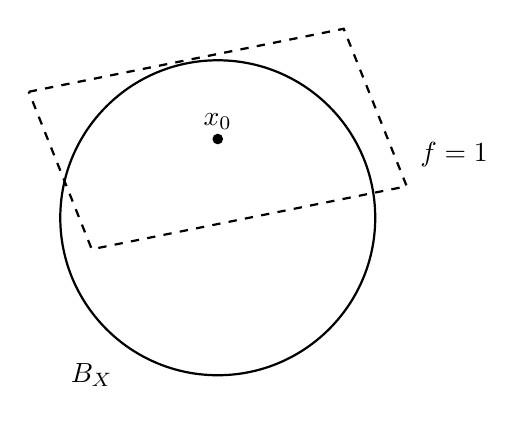
\begin{tikzpicture}[scale=2]

    % Draw the ball B_X (as a circle, no shading)
    \draw[thick] (0,0) circle (1);  % The ball B_X
    
    % Label B_X
    \node at (-0.8,-1) {$B_X$};

    % Draw the tangent plane at an angle (as a parallelogram)
    \draw[thick, dashed] (-1.2,0.8) -- (0.8,1.2) -- (1.2,0.2) -- (-0.8,-0.2) -- cycle;  % Tangent plane (parallelogram)
    
    % Mark point x_0 on the ball and the tangent plane
    \filldraw[black] (0,0.5) circle (0.03) node[anchor=south] {$x_0$};

    % Label the tangent plane f=1
    \node at (1.5,0.4) {$f = 1$};
\end{tikzpicture}
\end{center}

\subsection{Bidual}%
\label{sub:bidual}

Let $X$ be a normed space. Then $X^{\ast\ast} = (X^\ast)^\ast$ is the \emph{bidual}\index{bidual} or \emph{second dual} of $X$.

For $x \in X$, define $\hat x$ on $X^\ast$ by $f \mapsto f(x)$, i.e. evaluation at $x$.

Then $\hat x$ is linear, and
\[
|\hat x(f)| = |f(x)| \leq \|f\| \|x\|,
\]
for all $f \in X^\ast$. So $\hat x \in X^{\ast\ast}$, and $\|\hat x\| \leq \|x\|$. The map $x \mapsto \hat x$ is the \emph{canonical embedding} of $X$ into $X^{\ast\ast}$.

\begin{theorem}
	The canonical embedding is an isometric isomorphism of $X$ into $X^{\ast\ast}$.
\end{theorem}

\begin{proofbox}
	Linearity: note
	\begin{align*}
		\widehat{\lambda x + \mu y}(f) &= f(\lambda x + \mu y) = \lambda f(x) + \mu f(y) \\
					       &= (\lambda \hat x + \mu \hat y)(f).
	\end{align*}
	Isometric: for $x \in X$,
	\[
		\|\hat x\| = \sup\{|f(x)| \mid f \in B_{X^\ast} \} = \|x\|,
	\]
	by Hahn-Banach.
\end{proofbox}

\begin{remark}
	\begin{enumerate}
		\item[]
		\item Note that
			\[
			\langle f, \hat x \rangle = \langle x, f \rangle,
			\]
			for $x \in X$, $f \in X^\ast$.
		\item $\hat X = \{\hat x \mid x \in X \} \cong X$. Therefore,
			\[
				\hat X \text{ is closed in } X^{\ast\ast} \iff X \text{ is complete}.
			\]
		\item In general, the closure in $X^{\ast\ast}$ of $\hat X$ is a Banach space containing an isometric copy of $X$ as a dense subspace.
	\end{enumerate}
\end{remark}

\begin{definition}
	A normed space $X$ is \emph{reflexive}\index{reflexive} if the canonical embedding $X \to X^{\ast\ast}$ is surjective.
\end{definition}

\begin{exbox}
	\begin{enumerate}
	\item Any finite-dimensional space is reflexive.
	\item $\ell_p$ for $1 < p < \infty$ is reflexive.
	\item 	Any Hilbert space is reflexive.
	\item $L_p(\mu)$ for $1 < p < \infty$ is reflexive.
	\item $c_0, \ell_1, \ell_\infty, L_1([0, 1])$ are not reflexive.
\end{enumerate}
\end{exbox}

\begin{remark}
	If $X$ is reflexive, then $X$ is a Banach space, and $X \cong X^{\ast\ast}$.

	However, there exists a Banach space $X$ such that $X \cong X^{\ast\ast}$, but $X$ is not reflexive. So even though $\ell_p^{\ast\ast} \cong \ell_q^\ast \cong \ell_p$, this is not enough to show $\ell_p$ is reflexive.
\end{remark}


% lecture 3

\subsection{Dual Operators}%
\label{sub:dual_op}

Let $X, Y$ be normed spaces. Then,
\[
	\mathcal{B}(X, Y) = \{T : X \to Y \mid T \text{ linear, bounded}\}.
\]
Recall that $\mathcal{B}(X, Y)$ is a normed space with the operator norm:
\[
	\|T\| = \sup \{ \|Tx\| \mid x \in B_X\}.
\]
If $Y$ is complete, then $\mathcal{B}(X, Y)$ is complete.

For $T \in \mathcal{B}(X, Y)$, its \emph{dual operator}\index{dual operator} $T^\ast : Y^\ast \to X^\ast$ is given by
\[
T^\ast(g) = g \circ T.
\]
This is well-defined, and in the bracket notation
\[
\langle x, T^\ast g \rangle = \langle T x, g \rangle.
\]
It is easy to see that $T^\ast$ is linear, and moreover it is bounded. Note
\begin{align*}
	\|T^\ast\| &= \sup_{g \in B_{Y^\ast}} \|T^\ast g\| = \sup_{g \in B_{Y^\ast}} \sup_{x \in B_X} | \langle x, T^\ast g \rangle| = \sup_{x \in B_X} \sup_{g \in B_{Y^\ast}} | \langle Tx, g \rangle | \\
		   &\overset{HB}= \sup_{x \in B_x} \|Tx\| = \|T\|.
\end{align*}

\begin{remark}
	If $X, Y$ are Hilbert spaces, and we identify $X, Y$ with $X^\ast, Y^\ast$ respectively, then $T^\ast$ becomes the \emph{adjoint}\index{adjoint} of $T$.
\end{remark}

\begin{exbox}
	If $1 \leq p < \infty$, and $R : \ell_p \to \ell_p$ is the right-shift, then $R^\ast : \ell_q \to \ell_q$ is the left-shift.
\end{exbox}

We have the following properties:
\begin{itemize}
	\item $(\id_X)^\ast = \id_{X^\ast}$.
	\item $(\lambda S + \mu T)^\ast = \lambda S^\ast + \mu T^\ast$.
	\item $(ST)^\ast = T^\ast S^\ast$.
	\item $T \mapsto T^\ast : \mathcal{B}(X, Y) \to \mathcal{B}(Y^\ast, X^\ast)$ is an into isometric isomorphism.
	\item The following diagram commutes:
		\[
		\begin{tikzcd}
			X \arrow[r, "T"] \arrow[d] & Y \arrow[d] \\
			X^{\ast\ast} \arrow[r, "T^{\ast\ast}"] & Y^{\ast\ast}
		\end{tikzcd}
		\]
		In other words $\widehat{T x} = T^{\ast\ast} \hat x$, for all $x \in X$.
\end{itemize}

Indeed, for all $x \in X$, $g \in Y^\ast$,
\begin{align*}
	\braket{g, T^{\ast\ast} \hat x} &= \langle T^{\ast} g, \hat x \rangle = \langle x, T^{\ast} g\rangle \\
					       &= \langle Tx, g\rangle = \langle g, \widehat{Tx}\rangle.
\end{align*}

\subsection{Quotient spaces}%
\label{sub:qp}

Let $X$ be a NVS and $Y$ be a closed subspace. Then $X/Y$ is a normed space in the \emph{quotient norm}\index{quotient norm}:
\[
	\|x + Y\| = \inf\{ \|x + y\| \mid y \in Y\} = d(x, Y).
\]
Here closed is important, so that $\|x + Y\| = 0 \implies x \in Y$.

The quotient map $q : X \to X/Y$ is linear, surjective and bounded with $\|q\| = 1$, since for $x \in X$ 
\[
\|q(x)\| \leq \|x\|.
\]
Letting $D_X$ be the open unit ball of $X$, we can show $q(D_X) = D_{X/Y}$. Indeed if $x \in D_X$, then $\|q(x)\| \leq \|x\| < 1$. If $\|x + Y\| < 1$, then there exists $y \in Y$ with $\|x + y\| < 1$. So $x + y \in D_X$ and $q(x + y) = x + Y$.

So $\|q\| = 1$, unless $Y = X$. Also, $q$ is an open map.

Assume $T : X \to Z$ is a bounded linear map, and $Y \subseteq \ker T$. Then there exists a unique map $\tilde T : X/Y \to Z$ such that the following diagram commutes:
\[
\begin{tikzcd}
	X \arrow[rr, "T"] \arrow[dr, "q"] & & Z \\
					  & X/Y \arrow[ur, "\tilde T"] &
\end{tikzcd}
\]
Moreover, $\tilde T$ is linear and bounded, and $\|\tilde T\| = \|T\|$, since
\[
\tilde T(D_{X/Y}) = \tilde T(q(D_X)) = T(D_X).
\]

\begin{theorem}
	Let $X$ be a normed space. If $X^\ast$ is separable, then so is $X$.
\end{theorem}

\begin{remark}
	The converse is false in general, by taking $X = \ell_1$, then $X^\ast = \ell_\infty$.
\end{remark}

\begin{proofbox}
	Since $X^\ast$ is separable, so is $S_{X^\ast}$. Let $(f_n)$ be a dense sequence in $S_{X^\ast}$. For all $n \in \mathbb{N}$, choose $x_n \in B_X$ such that $|f_n(x_n)| > 1/2$.

	Set $Y = \overline{\spn}\{x_n \mid n \in \mathbb{N}\}$, the closed linear span of $x_n$ Then we claim $Y = X$.

	Assume not. Then we first find $f \in S_{X^\ast}$ such that $f|_Y = 0$. Since $X/Y \neq \{0\}$, we have $(X/Y)^\ast \neq \{0\}$, by Hahn-Banach. Choose any $g \in S_{(X/Y)^\ast}$.

	Let $f = g \circ q$. Then $\|f\| = \|g\| = 1$, so $f \in S_{X^\ast}$, and $f|_Y = 0$.

	Choose $n \in \mathbb{N}$ such that $\|f - f_n\| < 1/10$. Now,
	\begin{align*}
		\frac{1}{2} &< |f_n(x_n)| = |(f_n - f)(x_n)| \leq \|f_n - f\| \cdot \|x_n\| < \frac{1}{10},
	\end{align*}
	a contradiction.
\end{proofbox}

\begin{theorem}
	Let $X$ be a separable normed space. Then $X$ is isometrically isomorphic to a subspace of $\ell_\infty$.
\end{theorem}

Consider a map $T : X \to \ell_\infty$. The $n$'th coordinate is then a linear function of $x$, that is bounded, hence is a functional. So we can think of
\[
Tx = (f_n(x)).
\]
We also want $\|Tx\|_\infty = \|x\|$, which we can do by choosing a norming functional (or an appropriate approximate).

\begin{proofbox}
	Let $(x_n)$ be a dense sequence in $X$. For each $n \in \mathbb{N}$, choose $f_n \in S_{X^\ast}$ such that $f_n(x_n) = \|x_n\|$.

	Define $T : X \to \ell_\infty$ by
	\[
		T(x) = (f_1(x), f_2(x), \ldots).
	\]
	Note that $|f_n(x)| \leq \|x\|$, so $T$ is well-defined, linear and bounded with norm at most 1.

	But for each $n$,
	\[
	\|Tx_n\|_{\infty} \geq |f_n(x_n)| = \|x_n\|,
	\]
	so $\|Tx_n\|_{\infty} = \|x_n\|$. Since $(x_n)$ is dense, and continuity of $T$, we have $\|Tx\| = \|x\|$ for all $x \in X$.
\end{proofbox}

\begin{remark}
	We say that $\ell_\infty$ is \emph{isometrically universal}\index{isometrically universal} for the class $\mathcal{SB}$ of all separable Banach spaces.
\end{remark}

\begin{theorem}[Vector-valued Liouville's Theorem]
	Let $X$ be a complex Banach space, and $f : \mathbb{C} \to X$ bounded and holomorphic. Then $f$ is constant.
\end{theorem}

\begin{proofbox}
	Since $f$ is bounded, there is $M \in \mathbb{R}$ such that for all $z \in \mathbb{C}$, $\|f(z)\| \leq M$.

	$f$ is holomorphic means that
	\[
	\lim_{w \to z} \frac{f(w) - f(z)}{w - z}
	\]
	exists, and is denoted by $f'(z)$, for all $z \in \mathbb{C}$.

	Fix $\phi \in X^\ast$. Since $\phi$ is linear and continuous,
	\[
	\lim_{w \to z} \frac{\phi(f(w)) - \phi(f(z))}{w - z} = \phi \left( \lim_{w \to z} \frac{f(w) - f(z)}{w - z} \right).
	\]
	So $\phi \circ f : \mathbb{C} \to \mathbb{C}$ is entire.

	Also, for all $z \in \mathbb{C}$, $|\phi(f(z))| \leq \|\phi\| \cdot \|f(z)\| \leq M \dot \|\phi\|$. So by Liouville, $\phi \circ f$ is constant, hence $\phi(f(z)) =\phi(f(0))$ for all $z \in \mathbb{C}$.

	Fix $z \in \mathbb{C}$. Since $X^\ast$ separates the points of $X$, $f(z) = f(0)$.
\end{proofbox}

% lecture 4

\subsection{Locally Convex Spaces}%
\label{sub:lcs}

\begin{definition}
	A \emph{locally convex space}\index{locally convex space} (LCS) is a pair $(X, \mathcal{P})$ where $X$ is a real or complex vector space, and $\mathcal{P}$ is a family of seminorms on $X$ such that $\mathcal{P}$ separates the points of $X$, i.e. for all $x \in X \setminus \{0\}$, there exists $p \in \mathcal{P}$ with $p(x) \neq 0$.
\end{definition}

The family $\mathcal{P}$ defines a topology on $X$ as follows: $U \subseteq X$ is open if and only if, for all $x \in U$, there are seminorms $p_1, \ldots, p_n \in \mathcal{P}$ and $\eps > 0$ such that
\[
	\{y \in X \mid p_k(y - x) < \eps \text{ for } k = 1, \ldots, n\} \subseteq U.
\]
So the open balls form a base of the topology.

\begin{remark}
	\begin{enumerate}[1.]
		\item[]
		\item Addition and scalar multiplication are continuous.
		\item This is Hausdorff, as $\mathcal{P}$ separates the points.
		\item $x_n \to x$ in $X$ if and only if $p(x_n - x) \to 0$ for all $p \in \mathcal{P}$.
		\item Let $Y$ be a subspace of $X$. Let $\mathcal{P}_Y = \{p|_Y \mid p \in \mathcal{P}\}$. Then $(Y, \mathcal{P}_Y)$ is a LCS, and the topology of $(Y, \mathcal{P}_Y)$ is the subspace topology induced by the topology of the LCS $(X, \mathcal{P})$.
		\item Let $\mathcal{P}, \mathcal{Q}$ be two families ofseminorms on $X$, both separating points of $X$. Say $\mathcal{P}, \mathcal{Q}$ are \emph{equivalent}\index{equivalent seminorms}, and we write $P \sim Q$, if they generate the same topology on $X$.

			The topology of a LCS $(X, \mathcal{P})$ is metrizable if and only if there is a countable $Q \sim P$.
	\end{enumerate}
\end{remark}

\begin{definition}
	A \emph{Fr\'echet space}\index{Fr\'echet space} is a complete metrizable LCS.
\end{definition}

\begin{exbox}
	\begin{enumerate}
		\item A normed space $(X, \|\cdot\|)$ is a LCS with $\mathcal{P} = \{\|\cdot\|\}$.
		\item Let $U \subseteq \mathbb{C}$ be a non-empty open set, and
			\[
				\mathcal{O}(U) = \{ f : U \to \mathbb{C} \mid f \text{ holomorphic}\}.
			\]
			For $K \subseteq U$, $K$ compact, let
			\[
			p_K(f) = \sup_{z \in K} |f(z)|,
			\]
			for $f \in \mathcal{O}(U)$. Let $\mathcal{P} = \{p_K \mid K \subseteq U, K \text{ compact}\}$. Then $(\mathcal{O}(U), \mathcal{P})$ is a LCS. The topology is the topology of local uniform convergence.

			Note that there exists $(K_n)$ of compact subsets of $U$ such that $K_n \subseteq \mathrm{int} K_{n+1}$ for all $n$, and $\bigcup K_n = U$, and
			\[
				\{ p_{K_n} \mid n \in \mathbb{N}\} \sim \mathcal{P}.
			\]
			So $(\mathcal{O}(U), \mathcal{P})$ is metrizable, and in fact a Fr\'echet space. This topology is not normable, i.e. there is no norm on $\mathcal{O}(U)$ inducing the same topology (can use Montel's theorem).
		\item Take $d \in \mathbb{N}$, and $\Omega \subseteq \mathbb{R}^d$ non-empty and open. Take
			\[
				C^\infty(\Omega) = \{f : \Omega \to \mathbb{R} \mid f \text{ infinitely differentiable}\}.
			\]
			For a multiindex $\alpha = (\alpha_1, \ldots, \alpha_n)$, we have a differential operator $D^\alpha$ given by
			\[
			D^\alpha f = \left( \frac{\partial}{\partial x^1} \right)^{\alpha_1} \cdots \left( \frac{\partial}{\partial x^n} \right)^{\alpha_n}.
			\]
			For $\alpha \in (\mathbb{Z}_{\geq 0})^d$, $K \subseteq \Omega$ compact, define
			\[
				p_{K, \alpha}(f) = \sup\{ |(D^\alpha)f(x)| \mid x \in K\}.
			\]
			Let $\mathcal{P} = \{p_{K, \alpha} \mid \alpha \text{ multiindex}, K \text{ compact}\}$. Then $(C^\infty(\Omega), \mathcal{P})$ is a LCS, which is a Fr\'echet space that is not normable.
	\end{enumerate}
	
\end{exbox}

\begin{lemma}
	Let $(X, \mathcal{P})$ and $(Y, \mathcal{Q})$ be LCS, and $T : X \to Y$ a linear map. Then the following are equivalent:
	\begin{enumerate}[\normalfont(i)]
		\item $T$ is continuous.
		\item $T$ is continuous at $0$.
		\item For all $q \in \mathcal{Q}$, there are seminorms $p_1, \ldots, p_n \in \mathcal{P}$ and $C \geq 0$ such that for all $x$,
			\[
			q(Tx) \leq C \max_{1 \leq k \leq n} p_k(x).
			\]
	\end{enumerate}
\end{lemma}

\begin{proofbox}
	It is easy to see (i) $\iff$ (ii), since translations are a homeomorphism.

	We show (ii) $\implies$ (iii). Let $q \in \mathcal{Q}$, and $V = \{y \in Y \mid q(y) < 1\}$ a neighbourhood of $0$ in $Y$. As $T$ is continuous at $0$, there exists a neighbourhood of 0 in $X$ such that $T(U) \subseteq V$. Without loss of generality,
	\[
		U = \{x \in X \mid p_k(X) \leq \eps, k = 1, \ldots, n\}
	\]
	for some $n \in \mathbb{N}$, and $p_1, \ldots, p_n \in \mathcal{P}$, $\eps > 0$.

	Let $p(x) = \max_{1 \leq k \leq n} p_k(x)$. We show that $q(Tx) \leq \frac{1}{\eps} p(x)$ for all $x \in X$. Let $x \in X$. If $p(x) \neq 0$, then
	\[
	p \left( \frac{\eps x}{p(x)} \right) = \eps,
	\]
	so
	\[
	\frac{\eps x}{p(x)} \in U \implies T \left( \frac{\eps x}{p(x)} \right) \in V.
	\]
	Therefore,
	\[
	q \left( T \left( \frac{\eps x}{ p(x)} \right) \right) < 1 \implies q(Tx) \leq \frac{1}{\eps} p(x).
	\]
	If $p(x) = 0$, then $\lambda x \in U$ for all scalars $\lambda$, hence $q(T(\lambda x)) < 1$ for all $\lambda$. So $q(Tx) = 0$.

	Now we show (iii) $\implies$ (ii). Let $V$ be an open neighbourhood of $0$ in $Y$. We seek a neighbourhood $U$ of $0$ in $X$ such that $T(U) \subseteq V$. Without loss of generality,
	\[
		V = \{y \in Y \mid q_k(y) < \eps, k = 1, \ldots, m\}.
	\]
	For each $k= 1, \ldots, m$, there exist seminorms $p_{k,1}, \ldots, p_{k,n_k} \in \mathcal{P}$ and $C_k > 0$ such that for all $x \in X$,
	\[
	q_k(Tx) \leq C_k \max_{1 \leq j \leq n_k} p_{k, j}(x).
	\]
	Then,
	\[
		U = \{x \in X \mid p_{k, j}(x) \leq \frac{\eps}{C_k}, k = 1, \ldots, m, j =1, \ldots, n_k \}
	\]
	is a neighbourhood of $0$ in $X$, and for each $x \in U$,
	\[
	q_k(Tx) \leq C_k \max_{1 \leq j \leq n_k} p_{k, j}(x) < \eps
	\]
	for each $k = 1, \ldots, m$, so $Tx \in V$,
\end{proofbox}

\begin{definition}
	The \emph{dual space}\index{dual space of LCS} of a LCS $(X, \mathcal{P})$ is the space $X^\ast$ of all linear functional of $X$ which are continuous with respect to the topology of $X$.
\end{definition}

\begin{lemma}
	Let $f$ be a linear functional on a LCS $X$. Then,
	\[
		f \in X^\ast \iff \ker f\text { is closed}.
	\]
\end{lemma}

\begin{proofbox}
	One way is obvious: if $f$ is continuous, then $\ker f = f^{-1}(\{0\})$ must be closed.

	Now consider the other direction. We can assume without loss of generality that $f \neq 0$. Fix $x_0 \in X \setminus \ker f$. Since $\ker f$ is closed, there is a neighbourhood $U$ of $0$ in $X$, such that $x_0 + U$ is disjoint from $\ker f$.

	Without loss of generality,
	\[
		U = \{x \in X \mid p_k(x) < \eps, k = 1, \ldots, n\}
	\]
	for seminorms $p_1, \ldots, p_n \in \mathcal{P}$.

	Note that $U$ is convex and \emph{balanced}\index{balanced} (if $x \in U$, $|\lambda| = 1$ a scalar then $\lambda x \in U$) since $p_i$ are seminorms.

	As $f$ is linear, $f(U)$ is also convex and balanced. Hence it is an interval or a disc.

	But since $-f(x_0) \not \in f(U)$, otherwise $0 \in f(x_0 + U)$, $f(U)$ is bounded. Hence
	\[
		f(U) \subseteq \{\lambda \text{ a scalar} \mid |\lambda| < M\}.
	\]
	Hence for any $\delta > 0$,
	\[
		f \left( \frac{\delta}{M} U\right) \subseteq \{\lambda \text{ a scalar} \mid |\lambda| < \delta\},
	\]
	and $\frac{\delta}{M} U$ is a neighbourhood of $0$. Thus $f$ is continuous at $0$.
\end{proofbox}

% lecture 5

\begin{theorem}[Hahn-Banach]
	Let $(X, \mathcal{P})$ be a LCS.
	\begin{enumerate}[\normalfont(i)]
		\item If $Y$ is a subspace of $X$ and $g \in Y^\ast$, then there exists $f \in X^\ast$ such that $f|_Y = g$.
		\item If $Y$ is a closed subspace of $X$ and $x_0 \in X \setminus Y$, then there exists $f \in X^\ast$ such that $f|_Y = 0$, and $f(x_0) \neq 0$.
	\end{enumerate}
\end{theorem}

\begin{proofbox}
	

	(i) By lemma 1.1, there exists $p_1, \ldots, p_n \in \mathcal{P}$, and $C \geq 0$ such that for all $y \in Y$,
	\[
	|g(y)| \leq C \max_{1 \leq k \leq n} p_k(y).
	\]
	Define $p : X \to \mathbb{R}$ by
	\[
	p(x) = C \max_{1 \leq k \leq n} p_k(x).
	\]
	Then $p$ is a seminorm on $X$, and on $Y$ $|g(y)| \leq p(y)$ for all $y \in Y$.

	By Hahn-Banach on seminorms, there exists a linear functional $f$ on $X$ such that $f|_Y = g$ and for all $x \in X$, $|f(x)| \leq p(x)$. Lemma 1.1 gives us that $f$ is continuous.

	(ii) Let $Z = \spn(Y \cup \{x_0\})$. Define a linear functional $g$ on $Z$ by
	\[
	g(y + \lambda x_0) = \lambda
	\]
	for $y \in Y$, $\lambda$ a scalar. Notice that $\ker g = Y$ is closed by supposition, so $g$ is continuous, i.e. $g \in Z^\ast$. Then applying (i), we find $f \in X^\ast$ satisfying $f|_Z = g$, so in particular $f|_Y = 0$ and $f(x_0) = g(x_0) = 1$.
\end{proofbox}

\begin{remark}
	$X^\ast$ separates the points of $X$: given $x \neq y$, apply (ii) to $Y = \{0\}$, and $x_0 = x - y$.
\end{remark}

\newpage

\section{Dual Spaces of \texorpdfstring{$L_p(\mu)$}{Lp(mu)} and \texorpdfstring{$C(K)$}{C(K)}}%
\label{sec:ds}

Let $(\Omega, \mathcal{F}, \mu)$ be a measure space, and let $1 \leq p < \infty$. Recall
\[
	L_p(\mu) = \left\{f : \Omega \to \text{scalars} \biggm| f \text{ measurable}, \int_{\Omega} |f|^p \diff \mu < \infty\right\}.
\]
This is a normed space in the $L_p$-norm,
\[
\|f\|_p = \left( \int_{\Omega} |f|^p \diff \mu \right)^{1/p}.
\]
We identify functions $f, g$ if $f = g$ almost everywhere. If $p = \infty$, then
\[
	L_\infty(\mu) = \{f : \Omega \to \text{scalars} \mid f \text{ measurable, essentially bounded}\}.
\]
Essentially bounded means $f$ is bounded, up to a null set. This is a normed space in the $L_\infty$ norm:
\[
	\|f\|_\infty = \mathrm{ess} \sup |f| = \inf \{ \sup_{\Omega \setminus N} |f| \mid N \in \mathcal{F}, \mu(N) = 0\}.
\]
The infimum can be attained by taking $N_i$ that limit to the infimum, and then taking their union.

\begin{remark}
	If $\|\cdot\|$ is a seminorm on a vector space $X$, then
	\[
		N = \{x \in X \mid \|x\| = 0\}
	\]
	is a subspace of $X$, and $\|x + N\| = \|x\|$ defines a norm on the quotient.
\end{remark}

We will not think like this for $L_p$.

\begin{theorem}
	$L_p(\mu)$ is a Banach space for $1 \leq p \leq \infty$.
\end{theorem}

Our aim is to describe $L_p(\mu)^\ast$.

\subsection{Complex Measures}%
\label{sub:comp_m}

Let $\Omega$ be a set, and $\mathcal{F}$ be a $\sigma$-algebra on $\Omega$. A \emph{complex measure}\index{complex measure} on $\mathcal{F}$ is a countably additive set function $\nu : \mathcal{F} \to \mathbb{C}$.

The \emph{total variation measure}\index{total variation measure} of $\nu$, denoted by $|\nu|$, is defined as follows: for $A \in \mathcal{F}$,
\[
	|\nu|(A) = \sup \left\{  \sum_{k = 1}^n |\nu(A_k)| \biggm| A = \bigcup_{k = 1}^n A_k \text{ is a measurable partition of } A \right\}.
\]
Then $|\nu| : \mathcal{F} \to [0, \infty]$ is a positive measure, and is the smallest measure such that for all $A \in \mathcal{F}$,
\[
|\nu(A)| \leq |\nu|(A).
\]
In other words, if $\mu$ is a positive measure on $\mathcal{F}$ and for all $A \in \mathcal{F}$, $|\nu(A)| \leq \mu(A)$, then $|\nu|(A) \leq \mu(A)$.

The \emph{total variation}\index{total variation} of $\nu$ is
\[
\|\nu\|_1 = |\nu|(\Omega).
\]
As currently defined this could be infinite, but we will see that this is always finite.

$\nu$ satisfies the two continuity conditions:
\begin{itemize}
	\item If $A_n \subseteq A_{n+1}$, then
		\[
		\nu\left( \bigcup_{n = 1}^\infty A_n \right) = \lim_{n \to \infty} \nu(A_n).
		\]
	\item If $A_n \supseteq A_{n+1}$, then
		\[
		\nu\left( \bigcap_{n = 1}^\infty A_n \right) = \lim_{n \to \infty} \nu(A_n).
		\]
\end{itemize}

\emph{Signed measures}\index{signed measures} are complex measures that take real values, i.e. countably additive set functions $\mathcal{F} \to \mathbb{R}$.

\begin{theorem}
	Let $(\Omega, \mathcal{F})$ be as before, and $\nu$ a signed measure on $\mathcal{F}$.

	Then there exists a measurable partition $\Omega = P \cup N$ of $\Omega$ such that for all $A \in \mathcal{F}$ and $A \subseteq P$, then $\nu(A) \geq 0$, and if $A \subseteq N$ then $\nu(A) \leq 0$.
\end{theorem}

\begin{remark}
	\begin{enumerate}
		\item[]
		\item $\Omega = P \cup N$ is the \emph{Hahn decomposition}\index{Hahn decomposition} of $\Omega$ (or of $\nu$).
		\item Let $\nu^+(A) = \nu(A \cap P)$ and $\nu^-(A) = - \nu(A \cap N)$ for $A \in \mathcal{F}$.

			Then $\nu^+$, $\nu^-$ are finite positive measures such that $\nu = \nu^+ - \nu^-$, and $|\nu| = \nu^+ + \nu^-$.

			These properties determine $\nu^+$ and $\nu^-$ uniquely. This decomposition $\nu = \nu^+ - \nu^-$ is the \emph{Jordan decomposition}\index{Jordan decomposition} of $\nu$.
		\item Let $\nu$ be a complex measure. Then $\Re (\nu)$ and $\Im(\nu)$ are signed measures with Jordan decompositions $\nu_1 - \nu_2$ and $\nu_3 - \nu_4$. Then,
			\[
			\nu = \nu_1 - \nu_2 + i(\nu_3 - \nu_4).
			\]
			This is the \emph{Jordan decomposition} of $\nu$. Note that $\nu_k \leq |\nu|$, and
			\[
			|\nu| \leq \nu_1 + \nu_2 + \nu_3 + \nu_4.
			\]
			So $|\nu|$ is a finite measure since $\nu_1, \nu_2, \nu_3, \nu_4$ are all finite, so $\|\nu\|_1 < \infty$.
		\item Suppose the signed measure $\nu$ has Hahn decomposition $\Omega = P \cup N$ and Jordan decomposition $\nu^+ - \nu^-$. For $A, B \in \mathcal{F}$ with $B \subseteq A$,
			\[
			\nu^+(A) \geq \nu^+(B) \geq \nu(B),
			\]
			and $\nu^+(A) = \nu(B)$ if $B = P \cap A$. So,
			\[
				\nu^+(A) = \sup \{ \nu(B) \mid B \in \mathcal{F}, B \subseteq A\}.
			\]
	\end{enumerate}
\end{remark}

\begin{proofbox}
	This is a non-examinable sketch.

	Define
	\[
		\nu^+(A) = \sup \{\nu(B) \mid B \in \mathcal{F}, B \subseteq A\} \geq 0,
	\]
	since we may always take $B = \emptyset$. It is clear that $\nu^+(\emptyset) = 0$, and $\nu^+$ is finitely additive.

	The main claim is that $\nu^+(\Omega) < \infty$. Assume not. Inductively construct $(A_n), (B_n)$ in $\mathcal{F}$ such that $A_0 = \Omega$, and if $\nu^+(A_{n-1}) = \infty$, pick $B_n \subseteq A_{n-1}$, with $\nu(B_n) > n$.

	Then pick either $A_n = B_n$ or $A_{n-1} \setminus B_n$ such that $\nu^+(A_n) = \infty$.

	We can then use continuity of $\nu$ to get a contradiction, by condition on whether $A_n = B_n$ eventually, or $A_n = A_{n-1} \setminus B_n$ infinitely often.

	The next claim is that the supremum is achieved, so there exists $P \in \mathcal{F}$ such that
	\[
		\nu^+(\Omega) = \nu(P).
	\]
	Choose $A_n \in \mathcal{F}$, with $\nu(A_n) > \nu^+(\Omega) - 2^{-n}$, and we can check
	\[
	P = \bigcup_m \bigcap_{n \geq m} A_n
	\]
	works. Then letting $N = \Omega \setminus P$, we can check this works as a partition.
\end{proofbox}

% lecture 6

\begin{definition}
	Fix a measure space $(\Omega, \mathcal{F}, \mu)$. A complex measure $\nu : \mathcal{F} \to \mathbb{C}$ is \emph{absolutely continuous}\index{absolute continuous} with respect to $\mu$, written $\nu \ll \mu$, if for all $A \in \mathcal{F}$,
	\[
	\mu(A) = 0 \implies \nu(A) = 0.
	\]
\end{definition}

\begin{remark}
	\begin{enumerate}
		\item[]
		\item If $\nu \ll \mu$, then $|\nu| \ll \mu$. It follows that if $\nu = \nu_1 - \nu_2 + i \nu_3 - i \nu_4$ is the Jordan decomposition of $\nu_1$, then 
			\[
			\nu \ll \mu \iff \nu_k \ll \mu
			\]
			for all $k$ (note that $\nu_1, \nu_2$ are non-zero on different subsets of $\mathcal{F}$).
		\item If $\nu \ll \mu$, then for all $\eps > 0$, there exists $\delta > 0$ such that for any $A \in \mathcal{F}$,
			\[
			\mu(A) < \delta \implies |\nu(A)| < \eps.
			\]
	\end{enumerate}
\end{remark}

\begin{exbox}
	If $f \in L_1(\mu)$, then
	\[
	\nu(A) = \int_A f \diff \mu,
	\]
	for $A \in \mathcal{F}$, defines a complex measure on $\mathcal{F}$ (by dominated convergence), and $\nu \ll \mu$.
\end{exbox}

\begin{definition}
	A set $A \in \mathcal{F}$ is $\sigma$-finite with respect to $\mu$ if there exists $(A_n)$ in $\mathcal{F}$ such that
	\[
	A = \bigcup_{n \in \mathbb{N}} A_n, \qquad \mu(A_n) < \infty.
	\]
	We say that $\mu$ is $\sigma$-finite if $\Omega$ is a $\sigma$-finite set (so every $A \in \mathcal{F}$ is $\sigma$-finite).
\end{definition}

\begin{theorem}[Radon-Nikodym Theorem]
	Let $(\Omega, \mathcal{F}, \mu)$ be a $\sigma$-finite measure and $\nu : \mathcal{F} \to \mathbb{C}$ be a complex measure such that $\nu \ll \mu$.

	Then there exists a unique $f \in L_1(\mu)$ such that
	\[
	\nu(A) = \int_A f \diff \mu,
	\]
	for all $A \in \mathcal{F}$. Moreover $f$ takes values in $\mathbb{C}$ or $\mathbb{R}$ or $\mathbb{R}^+$ depending on whether $\nu$ is a complex/signed/positive measure.
\end{theorem}

\begin{proofbox}
	This is a non-examinable sketch.

	First we show uniqueness. This follows as if $f \in L_1(\mu)$ and $\int_A f \diff \mu = 0$, then $f = 0$ almost everywhere.

	For existence, first assume $\nu$ is a finite positive measure, by taking the Jordan decomposition.

	We can also assume $\mu$ is finite: for each partition $A_i$ we have function $f_i$, which we can glue together; this extends by monotone convergence, since we first assumed $\nu$ is finite and positive.

	Now let
	\[
		\mathcal{H} = \left\{h : \Omega \to \mathbb{R}^+ \biggm| \int_A h \diff \mu \leq \nu(A) \text{ for all } A \in \mathcal{F}\right\}.
	\]
	Note $0 \in \mathcal{H}$, $h_1, h_2 \in \mathcal{H} \implies h_1  \vee H_2 \in \mathcal{H}$, and if $h_n \in \mathcal{H}$, then $h_n \uparrow h \implies h \in \mathcal{H}$. Let
	\[
		\mathcal{L} = \sup \left\{ \int_{\Omega} h \diff \mu \biggm| h \in \mathcal{H} \right\}.
	\]
	This sup is attained (by monotone convergence). Hence there exists $f \in \mathcal{H}$ which attains $\mathcal{L}$. We show that
	\[
	\int_A f \diff \mu = \nu(A),
	\]
	for all $A \in \mathcal{F}$. The idea is that if there exists $A$ with
	\[
	\int_A f \diff \mu < \nu(A),
	\]
	then $f + \delta \mathbbm{1}_{A}$ should be in $\mathcal{H}$ for some $\delta > 0$, contradicting the maximality. However this doesn't quite work as we may fail the condition for $B \subseteq A$.

	For $n \in \mathbb{N}$, define
	\[
	\nu_n(A) = \nu(A) - \int_A f \diff \mu - \frac{1}{n} \mu(A) = \nu(A) - \int_A \left(f + \frac{1}{n} \right) \diff \mu,
	\]
	for all $A \in \mathcal{F}$. Now $\nu_n$ is a signed measure, so we get a Hahn decomposition
	\[
	\Omega = P_n \cup N_n.
	\]
	Then, $f + \frac{1}{n} \mathbbm{1}_{P_n} \in \mathcal{H}$, so $\mu(P_n) = 0$ to not contradict maximality.

	Let $P = \bigcup P_n$. Then $\mu(P) = 0$, so $\nu(P) = 0$ by absolute continuity.

	Set $N = \bigcap N_n$. Then,
	\begin{align*}
		\nu(A) &= \nu(A \cap N) = \nu_n(A \cap N) + \int_{A \cap N}  f \diff \mu + \frac{1}{n} \mu(A \cap N) \\
		       &\leq \int_A f \diff \mu + \frac{1}{n} \mu(A \cap N).
	\end{align*}
	Then we let $n \to \infty$.
\end{proofbox}

\begin{remark}
	\begin{enumerate}
		\item[]
		\item The proof shows that every complex measure $\nu : \mathcal{F} \to \mathbb{C}$ has a decomposition $\nu = \nu_1 + \nu_2$, where $\nu_1 \ll \mu$ and $\nu_2 \perp \mu$. This is the \emph{Lebesgue decomposition}\index{Lebesgue decomposition} of $\nu$.
		\item The unique $f \in L_1(\mu)$ in the Radon-Nikodym theorem is the \emph{Radon-Nikodym derivative}\index{Radon-Nikodym derivative} of $\nu$ with respect to $\mu$, denoted by $\diff \nu/ \diff \mu$. For measurable $g$, then $g$ is $\nu$-integrable if and only if $g \cdot \diff \nu/ \diff \mu$ is $\mu$-integrable, and
			\[
			\int_{\Omega} g \diff \nu = \int_{\Omega} g \frac{\diff \nu}{\diff \mu} \diff \mu.
			\]
	\end{enumerate}
\end{remark}

\subsection{Duals of \texorpdfstring{$L_p$}{Lp}}%
\label{sub:dlp}

Fix a measure space $(\Omega, \mathcal{F}, \mu)$, and let $1 \leq p < \infty$. Let $q$ be the conjugate index of $p$, and for $g \in L_q = L_q(\mu)$, define $\phi_g$ on $L_p$ by
\[
\phi_g(f) = \int_{\Omega} fg \diff \mu.
\]
By H\"older's, $fg \in L_1$, and
\[
|\phi_g(f)| \leq \|f\|_p \|g\|_q.
\]
So $\phi_g \in L_p^\ast$, and $\|\phi_g\| \leq \|g\|_q$. So $\phi : L_q \to L_p^\ast$ exists, given by $g \mapsto \phi_g$. This is linear and bounded, with $\|\phi\| \leq 1$.

\begin{theorem}
	Let $(\Omega, \mathcal{F}, \mu)$, and $p, q, \phi$ be as above.
	\begin{enumerate}[\normalfont(i)]
		\item If $1 < p < \infty$, then $\phi$ is an isometric isomorphic, so $L_p^\ast \cong L_q$.
		\item If $p = 1$ and $\mu$ is $\sigma$-finite, then $L_1^\ast \cong L_\infty$.
	\end{enumerate}	
\end{theorem}

\begin{proofbox}
	What remains is to check that $\phi$ is isometric and onto. Fix $g \in L_q$. We need to check that $\|\phi_g\| = \|g\|_q$.

	Let $\lambda : \Omega \to \text{scalars}$ be measurable, with $|\lambda| = 1$ and $\lambda \cdot g = |g|$, i.e. let $\lambda = \mathrm{sign}(g)$.

	For $1 < p < \infty$, let $f = \lambda |g|^{q-1}$. Then,
	\[
	\int_{\Omega} |f|^{p} \diff \mu = \int_{\Omega} |g|^{pq - p} \diff \mu = \int_{\Omega} |g|^q \diff \mu < \infty,
	\]
	so $f \in L_p$, and
	\[
	\|f\|_p = \|g\|_q^{q/p} = \|g\|_q^{q-1}.
	\]
	Then notice
	\[
	\phi_g(f) = \int \lambda g |g|^{q-1} \diff \mu = \|g\|_q^{q} = \|f\|_p \cdot \|g\|_q,
	\]
	so $\|\phi_g\| \geq \|g\|_q$.

	For $p = 1$, let $s < \|g\|_\infty$. Then $\mu(\{|g| > s\}) > 0$. Since $\mathcal{F}$ is $\sigma$-finite, there exists measurable $A \subseteq \{|g| > s\}$, such that $0 < \mu(A) < \infty$. Then $f = \lambda \mathbbm{1}_{A} \in L_1$, and $\|f\|_1 = \mu(A)$. Now,
	\[
	\|\phi_g\| \cdot \mu(A) \geq \phi_g(f) = \int_A |g| \diff \mu \geq s \mu(A).
	\]
	So $\|\phi_g\| \geq s$, and so $\|\phi_g\| \geq \|g\|_{\infty}$.

	The hard part is showing $\phi$ is onto. Fix $\psi \in L_p^\ast$. We seek $g \in L_q$ such that $\psi = \phi_g$.

	The idea is as follows: let $\psi(\mathbbm{1}_{A}) = \int_A g \diff \mu$. Then we can define $\nu(A) = \psi(\mathbbm{1}_{A})$ for $A \in \mathcal{F}$, with $\nu \ll \mu$, and apply Radon-Nikodym. But we have to split into cases to make this work.

	First, consider when $\mu$ is finite. For $A \in \mathcal{F}$, $\mathbbm{1}_{A} \in L_p$, so we can define $\nu(A) = \psi(\mathbbm{1}_{A})$. This is a measure, as if $A = \bigcup A_n$ is a measurable partition, then
	\[
	\sum_{n = 1}^N \mathbbm{1}_{A_n} \to \mathbbm{1}_{A}
	\]
	in $L_p$, by DCT. So,
	\[
	\sum_{n=1}^N \nu(A_n) = \psi \left( \sum_{n=1}^N \mathbbm{1}_{A_n} \right) \to \psi(\mathbbm{1}_{A}) = \nu(A).
	\]
	So $\nu$ is a complex/signed measure. If $\mu(A) = 0$, then $\mathbbm{1}_{A} = 0$ almost everywhere, so $\nu(A) = \psi(\mathbbm{1}_{A}) = 0$. Thus $\nu \ll \mu$. Hence by Radon-Nikodym, there exists $g \in L_1(\mu)$ such that
	\[
	\nu(A) = \int_A g \diff \mu,
	\]
% lecture 7
	for all $A \in \mathcal{F}$. We show that $g \in L_q(\mu)$ and $\psi = \phi_g$, i.e.
	\[
	\psi(f) = \int_{\Omega} fg \diff \mu
	\]
	for all $f \in L_p$. We have
	\begin{align*}
		\psi(\mathbbm{1}_{A}) &= \nu(A) = \int_A g \diff \mu = \int_{\Omega} \mathbbm{1}_{A} g \diff \mu,
	\end{align*}
	hence
	\[
	\psi(f) = \int_{\Omega} fg \diff \mu
	\]
	for all simple functions $f$. Given $f \in L_\infty$, there is a sequence $(f_n)$ of simple functions such that $f_n \to f$ in $L_\infty$. Then $f_n g \to f g$ in $L_1$ by dominated convergence, and $f_n \to f$ in $L_p$, as $\mu$ is finite. Thus
	\[
	\psi(f) = \lim_{n \to \infty} \psi(f_n) = \lim_{n \to \infty} \int_{\Omega} f_n g \diff \mu = \int_{\Omega} f g \diff \mu.
	\]
	Next we deduce that $g \in L_q$. Fix a measurable function $\lambda$ such that $|\lambda| = 1$ and $\lambda g = |g|$.

	Split into cases. For $p \neq 1$, let $A_n = \{|g| \leq n\}$. Then $f = \lambda \mathbbm{1}_{A_n} |g|^{q-1} \in L_\infty$, and
	\[
	\int_{A_n} |g|^q \diff \mu = \int_{\Omega} fg \diff qm = \psi(f) \leq \|\psi\| \cdot \|f\| = \|\psi\| \left(\int_{A_n} |g|^q \diff \mu \right)^{1/p},
	\]
	so
	\[
	\left( \int_{A_n} |g|^q \diff \mu \right)^{1/q} \leq \|\psi\|.
	\]
	Let $n \to \infty$, and use monotone convergence to get $g \in L_q$.

	For $p = 1$, fix $s > \|\psi\|$ and let $A = \{|g| > s\}$. Then $f = \lambda \mathbbm{1}_{A} \in L_\infty$, so
	\[
	s \mu(A) = \int_A |g| \diff \mu = \int_{\Omega} 
f g \diff \mu = \psi(f) \leq \|\psi\| \|f\|_1 = \|\psi\| \mu(A).
	\]
	The only way is if $\mu(A) = 0$, so $g \in L_\infty$.

	Hence, $\psi$ and $\phi_g$ are both in $L_p^\ast$, and $\psi = \phi_g$, on $L_\infty$. Since $L_\infty$ is dense in $L_p$, we get $\psi = \phi_g$. 
\end{proofbox}

Before we continue to our next cases when $\mu$ may not be finite, we need a few pieces notation.

Fix $A \in \mathcal{F}$. Then,
\[
	\mathcal{F}_A = \{B \in \mathcal{F} \mid B \subseteq A\}
\]
is a $\sigma$-algebra on $A$. Define $\mu_A = \mu|_{\mathcal{F}_A}$. Then $(A, \mathcal{F}_A, \mu_A)$ is a measure space, with $L_p(\mu_A) \subseteq L_p(\mu)$. Let
\[
\psi_A = \psi|_{L_p(\mu_A)}.
\]
Let's continue.

\begin{proofbox}
	Let $\psi_A = \psi|_{L_p(\mu_A)}$, the restriction onto a subset. Then $\psi_A \in L_p(\mu_A)^\ast$, and $\|\psi_A\| \leq \|\psi\|$.

	Let $A, B \in \mathcal{F}$ with $A \cap B = \emptyset$. In the case $1 < p < \infty$,
	\begin{align*}
		\|\psi_{A \cup B}\| &= \sup \{|\psi_{A \cup B}(h)| \mid h \in L_p(\mu_{A \cup B}), \|h\|_p \leq 1\} \\
				    &= \sup\{|\psi_A(f) + \psi_B(g)| \mid f \in L_p(\mu_A), g \in L_p(\mu_B), \|f\|_p^p + \|g\|_p^p \leq 1\} \\
				    &= \sup\{a |\psi_A(f)| + b |\psi_B(g)| \mid a, b \geq 0, a^p + b^p \leq 1, \\
				    & \qquad \qquad \qquad \qquad \qquad \qquad \qquad \qquad f \in B_{L_p}(\mu_A), g \in B_{L_p}(\mu_B)\} \\
				    &= \sup\{a \|\psi_A\| + b \|\psi_B\| \mid a, b \geq 0, a^p + b^p \leq 1\} \\
				    &= (\|\psi_A\|^q + \|\psi_B\|^q)^{1/q},
	\end{align*}
	since $(\ell_p^2)^\ast = \cong \ell_q^2$.

	The next case is when $\mu$ is $\sigma$-finite. We have a measurable partition $\Omega = \bigcup A_n$ of $\Omega$, with $\mu(A_n) < \infty$ for all $n$. By the first case, there is $g_n \in L_q(\mu_{A_n})$ with
	\[
	\psi_{A_n} = \phi_{g_n}.
	\]
	Define $g$ such that
	\[
	g|_{A_n} = g_n.
	\]
	When $p = 1$, then
	\[
	\|g\|_\infty = \sup_{n} \|g_n\|_\infty = \sup_n \|\psi_{A_n}\| \leq \|\psi\|.
	\]
	So $g \in L_q$. For $p \neq 1$, note
	\[
	\sum_{n = 1}^N \|g_n\|_q^q = \sum_{n = 1}^N \|\psi_{A_n}\|^q = \|\psi_{A_1 \cup \cdots \cup A_N}\|^q \leq \|\psi\|^q.
	\]
	By monotone convergence, $g \in L_q$. In both cases, $g \in L_q$, so $\phi_g \in L_p(\mu)^\ast$, and so we have
	\[
	\psi|_{L_p(\mu_{A_n})} = \psi_{A_n} = \phi_{g_n} = \phi_g |_{L_p(\mu_{A_n})}.
	\]
	Since $\bigcup L_p(\mu_{A_n})$ has dense linear span in $L_p(\mu)$, we find that $\psi = \phi_g$ on $L_p(\mu)$.

	The final case is for general $\mu$, and $1 < p < \infty$. Choose $(f_n)$ in $B_{L_p}$ such that $\|\psi\| = \lim_n |\psi(f_n)|$. For all $k, n$, note that
	\[
	\mu(|f_n| \geq 1/k) \leq k^p \|f_n\|_p^p < \infty,
	\]
	by Markov's inequality. Hence
	\[
		A = \bigcup_{n, k}\{|f_n| \geq 1/k\}
	\]
	is $\sigma$-finite, and for all $n$, $f_n = 0$ on $\Omega \setminus A$. So $\|\psi_A\| = \|\psi\|$. So,
	\[
	\|\psi_A\| = \|\psi\| = (\|\psi_A\|^q + \|\psi_{\Omega \setminus A}\|^q)^{1/q},
	\]
	and hence $\psi_{\Omega\setminus A} = 0$. Hence we are done by case 2.
\end{proofbox}

\begin{corollary}
	For $1 < p < \infty$, $L_p(\mu)$ is reflexive.
\end{corollary}

\begin{proofbox}
	Let $\phi \in L_p^{\ast\ast}$. We seek $f \in L_p$ such that $\phi = \hat f$, i.e.
	\[
	\phi(\psi) = \hat f(\psi) = \psi(f)
	\]
	for all $\psi \in L_p^\ast$, i.e.
	\[
	\phi(\phi_g) = \phi_g(f)
	\]
	for all $g \in L_q$. The map $g \mapsto \phi(\phi_g)$ is in $L_q^\ast$, so by the previous theorem, there exists $f \in L_p$ such that
	\[
	\phi(\phi_g) = \int_{\Omega} g f \diff \mu = \phi_g(f).
	\]
\end{proofbox}

\subsection{\texorpdfstring{$C(K)$}{C(K)} Spaces}%
\label{sub:ck_sp}

Throughout, we assume that $K$ is a compact Hausdorff space. Here we make a distinction on our base field:
\[
	C(K) = \{f : K \to \mathbb{C} \mid f \text{ continuous}\}.
\]
This is a complex Banach space with the $\|\cdot\|_\infty$ norm. We also denote
\[
	C^{\mathbb{R}}(K) = \{f : K \to \mathbb{R} \mid f \text{ continuous}\},
\]
and another important object is
\[
	C^+(K) = \{f : K \to \mathbb{R}^+ \mid f \text{ continuous}\},
\]
which is a subset of $C^{\mathbb{R}}(K)$ (more specifically a cone). Let
\[
	M(K) = C(K)^\ast =  \{ \phi : C(K) \to \mathbb{C} \mid \phi \text{ linear, bounded}\},
\]
and also we define
\[
	M^{\mathbb{R}}(K) = \{\phi \in M(K) \mid \phi(f) \in \mathbb{R} \text{ for all } f \in C^{\mathbb{R}}(K)\}.
\]
We do not define $M^{\mathbb{R}} = (C^{\mathbb{R}})^\ast$, however we will show this is true. Also define
\[
	M^+(K) = \{\phi : C(K) \to \mathbb{C} \mid \phi \text{ linear, for all } f \in C^+(K), \phi(f) \in \mathbb{R}^+\}.
\] 
We do note assume continuity, however we will show any $f \in M^+$ is continuous, so $M^+ \subseteq M^\mathbb{R}$. The members of this set are the \emph{positive linear functionals}\index{positive linear functionals}.

Our aim is to describe $M(K), M^{\mathbb{R}}(K)$. We will show that it is enough to describe $M^+(K)$.

\begin{lemma}
	\begin{enumerate}[\normalfont(i)]
		\item[]
\item For all $\phi \in M(K)$, there is a unique $\phi_1, \phi_2 \in M^{\mathbb{R}}(K)$ such that
	\[
	\phi = \phi_1 + i \phi_2.
	\]
	\item The map $\phi \mapsto \phi|_{C^{\mathbb{R}(K)}}$, from $M^{\mathbb{R}} \to (C^{\mathbb{R}})^\ast$ is an isometric isomorphism.
	\item $M^+(K) \subseteq M^\mathbb{R}(K)$ and
		\[
			M^+(K) = \{ \phi \in M(K) \mid \|\phi\| = \phi(1_K)\}.
		\]
	\item For all $\phi \in M^\mathbb{R}(K)$, there exists a unique $\phi^+, \phi^-$ such that
		\[
			\phi = \phi^+ - \phi^- \qquad \text{and} \qquad \|\phi\| = \|\phi^+\| + \|\phi^-\|.
		\]
\end{enumerate}
\end{lemma}

\begin{proofbox}
	

	(i) Define $\bar \phi : C(K) \to \mathbb{C}$, by
	\[
	\bar \phi(f) = \overline{\phi(\bar f)}.
	\]
	Then $\bar \phi \in M(K)$, and
	\[
	\phi \in M^{\mathbb{R}}(K) \iff \phi = \bar \phi.
	\]
	First we show uniqueness. If $\phi = \phi_1 + i \phi_2$, then $\bar f = \phi_1 - i \phi_2$, so
	\[
	\phi_1 = \frac{\phi + \bar \phi}{2}, \qquad \phi_2 = \frac{\phi - \bar \phi}{2i}.
	\]
	This also shows existence, by defining $\phi_1, \phi_2$ in this way.
% lecture 8

	(ii) Let $\phi \in M^{\mathbb{R}}$, and $\psi = \phi|_{C^{\mathbb{R}}}$. Note that $\psi \in (C^{\mathbb{R}})^{\ast}$, and moreover $\|\psi\| \leq \|\phi\|$.

	First we show this map is isometric. Let $f \in C(K)$, and $\lambda \in \mathbb{C}$ such that $|\lambda| = 1$ and $|\phi(f)| = \lambda \phi(f)$. Then,
	\begin{align*}
		|\phi(f)| &= \lambda \phi(f) = \phi(\lambda f) = \phi(\Re(\lambda f)) + i \underbrace{\phi(\Im(\lambda f))}_{0 \text{ as } \phi \in M^{\mathbb{R}}} \\
			  &= \phi(\Re(\lambda f)) = \psi(\Re(\lambda f)) \leq \|\psi\| \|\Re(\lambda f)\|_\infty \leq \|\psi\| \|f\|_\infty.
	\end{align*}
	So $\|\phi\| \leq \|\psi\|$. To show this map is onto, say we have $\psi \in (C^{\mathbb{R}})^{\ast}$. Then the obvious way to define $\phi$ is
	\[
	\phi(f) = \psi(\Re(f)) + i \psi(\Im(f)),
	\]
	for $f \in C(K)$. Then $\phi \in M(K)$ and $\phi|_{C^{\mathbb{R}}(K)} = \psi$.

	(iii) To show the inclusion, let $\phi \in M^{+}(K)$, and $f \in C^{\mathbb{R}}(K)$ with $-1 \leq f \leq 1$ on $K$. Then $1_K \pm f \geq 0$ on $K$. So,
	\[
	\phi(1_K \pm f) = \phi(1_K) \pm \phi(f) \geq 0.
	\]
	So $\phi(f) \in \mathbb{R}$, and $|\phi(f)| \leq \phi(1_K)$. Hence, $\phi|_{C^{\mathbb{R}}(K)} \in (C^{\mathbb{R}})^{\ast}$, and $\|\phi|_{C^{\mathbb{R}}(K)}\| = \phi(1_K)$.

	By (ii), this gives us that $\phi \in M^{\mathbb{R}}(K)$ and $\|\phi\| = \phi(1_K)$.

	This immediately shows that $M^{+}(K) \subseteq \{\phi \in M(K) \mid \|\phi\| = \phi(1_K)\}$. To show the other inclusion, let $\phi \in M(K)$ with $\|\phi\| = \phi(1_K)$. Scale so that $\phi(1_K) = 1$.

	Let $f \in C^{\mathbb{R}}(K)$, and $\phi(f) = a + ib$. For $f \in \mathbb{R}$,
	\begin{align*}
		|\phi(f + it 1_K)|^2 &= |a + i(b + t)|^2 = a^2 + b^2 + 2bt + t^2 \\
				     &\leq \|f + it1_K\|^2_\infty \leq \|f\|_\infty^2 + t^2.
	\end{align*}
	By looking at the degree 1 term, we get $b = 0$, so $\phi(f) \in \mathbb{R}$.

	Now let $f \in C^{+}(K)$. Without loss of generality, let $0 \leq f \leq 1$ on $K$. Then
	\[
	-1 \leq 1_K - 2f \leq 1,
	\]
	so we get
	\[
	\phi(1_K - 2f) = 1 - 2 \phi(f) \leq \|\phi\| \cdot \|1_K - 2f\|_\infty \leq 1,
	\]
	which gives $\phi(f) \geq 0$, as desired.

	(iv) We begin by motivating uniqueness, but will sidetrack to prove existence.

	Assume that $\psi^+, \psi^- \in M^{+}(K)$, $\phi = \psi^{+} - \psi^{-}$, and $\|\phi\| = \|\psi^{+}\| + \|\psi^{-}\|$.

	If $0 \leq g \leq f$ on $K$, then note
	\[
	\phi(g) \leq \psi^{+}(g) \leq \psi^{+}(f).
	\]
	So $\psi^{+}(f) \geq \sup\{\phi(g) \mid 0 \leq g \leq f\}$. This motivates our definition of $\phi^{+}$, $\phi^{-}$.

	We segue into proving existence. Define for $f \in C^{+}(K)$ 
	\[
		\phi^{+}(f) = \sup \{\phi(g) \mid 0 \leq g \leq f\}.
	\]
	Then we have
	\[
	|\phi(g)| \leq \|\phi\| \cdot \|g\|_\infty \leq \|\phi\| \cdot \|f\|_\infty,
	\]
	so the supremum exists. Moreover $\phi^{+}(f) \geq 0$ since we may take $g = 0$, and $\phi^{+}(f) \geq \phi(f)$ by taking $g = f$.

	Next it is easy to see that $\phi^{+}(\lambda f) = \lambda \phi^{+}(f)$ for all $f \in C^{+}(K)$ and $\lambda \in \mathbb{R}^+$. Moreover for $f_1, f_2 \in C^{+}(K)$,
	\[
	\phi^{+}(f_1 + f_2) = \phi^{+}(f_1) + \phi^{+}(f_2).
	\]
	Indeed, if $0 \leq g_1 \leq f_1$, and $0 \leq g_2 \leq f_2$, then $0 \leq g_1 + g_2 \leq f_1 + f_2$, showing that
	\[
	\phi^{+}(f_1 + f_2) \geq \phi(g_1 + g_2) = \phi(g_1) + \phi(g_2).
	\]
	Taking a supremum we get
	\[
	\phi^{+}(f_1 + f_2) \geq \phi^{+}(g_1 + g_2).
	\]
	For the other way around let $0 \leq g \leq f_1 + f_2$, and define
	\begin{align*}
		g_1 = g \wedge f_1, \qquad g_2 = g - g_1.
	\end{align*}
	Then $0 \leq g_1 \leq f_1$, and $0 \leq g_2 \leq f_2$. And hence
	\[
	\phi^{+}(f_1) + \phi^{+}(f_2) \geq \phi(g_1) + \phi(g_2) = \phi(g).
	\]
	Taking a supremum over all $g$, gives the other inequality. So $\phi^{+}$ is positively linear.

	Next we want to extend $\phi$ to $C^{\mathbb{R}}$. Given $f \in C^{\mathbb{R}}$, we can write $f = f_1 - f_2$ for some $f_1, f_2 \in C^{+}(K)$ (splitting into positive and negative parts). Then define
	\[
	\phi^{+}(f) = \phi^{+}(f_1) - \phi^{+}(f_2).
	\]
	Then we can show $\phi^{+}$ is well-defined and linear on $C^{\mathbb{R}}$, from the scaling and multiplicative properties we showed earlier.

	Finally define $\phi^{+} : C(K) \to \mathbb{C}$ by
	\[
	\phi^{+}(f) = \phi^{+}(\Re f) + i \phi^{+}(\Im f).
	\]
	Then $\phi^{+}$ is in $M^{+}(K)$. Now we can define $\phi^{-} = \phi^{+} - \phi$. For $f \in C^{+}(K)$, note that $\phi^{+}(f) \geq \phi(f)$, so $\phi^{-}(f) \leq 0$. Hence $\phi^{-} \in M^{+}(K)$ and $\phi = \phi^{+} - \phi^{-}$.

	Finally we show that the norms coincide. We have
	\[
	\|\phi\| \leq \|\phi^{+}\| + \|\phi^{-}\| = \phi^{+}(1_K) - \phi^{-}(1_K) = 2 \phi^{+}(1_K) - \phi(1_K).
	\]
	Fox some $0 \leq g \leq 1$, so $-1 \leq 2g - 1_K \leq 1$ on $K$. So,
	\[
	\phi(2g - 1_K) = 2\phi(g) - \phi(1_K) \leq \|\phi\|.
	\]
	Taking a supremum over $g$, we find
	\[
	2 \phi^{+}(1_K) - \phi(1_K) \leq \|\phi\|.
	\]
	Hence we get equality, and so
	\[
	\|\phi\| = \|\phi^{+}\| + \|\phi^{-}\|.
	\]

	Now we get back to uniqueness. Recall that if we have $\phi = \psi^{+} - \psi^{-}$, then we have shown $\psi^{+}(f) \geq \phi^{+}(f)$ for all $f \in C^{+}(K)$.

	This also implies that $\psi^{-}(f) \geq \phi^{-}(f)$. So we have
	\[
	\psi^{+} - \phi^{+}, \qquad \psi^{-} - \phi^{-} \in M^{+}(K).
	\]
	But hence we have
	\begin{align*}
		\|\phi\| &= \|\phi^{+}\| + \|\phi^{-}\| = \phi^+(1_K) + \phi^{-}(1_K) \\
			 &\leq \psi^+(1_K) + \psi^{-}(1_K) = \|\psi^{+}\| + \|\psi^{-}\| \\
			 &= \|\phi\|.
	\end{align*}
	So we have equality. Hence $\phi^{+}(1_K) = \psi^{+}(1_K)$, but then
	\[
	\|\psi^{+} - \phi^{+}\| = (\psi^{+} - \phi^{+})(1_K) = 0.
	\]
	So $\psi^{+} = \phi^{+}$, and $\psi^{-} = \phi^{-}$.
\end{proofbox}

Before starting the next discussion, we will need to go over a few topological preliminaries.

Recall that we have a fixed compact Hausdorff space $K$.
\begin{enumerate}
	\item $K$ is \emph{normal}\index{normal space} if given closed $E, F \subseteq K$, with $E \cap F = \emptyset$, then there exists open $U, V \subseteq K$ with $U \cap V = \emptyset$ such that $E \subseteq U, F \subseteq V$.

		Equivalently, given $E \subseteq U \subseteq K$, where $E$ is closed and $U$ is open, there exists open $V \subseteq K$ such that
		\[
		E \subseteq V \subseteq \overline{V} \subseteq U.
		\]
	\item Urysohn's lemma: if $E, F \subseteq K$ are closed and disjoint in a normal space, then there exists continuous $f : K \to [0, 1]$ such that $f = 0$ on $E$, and $f = 1$ on $F$.
	\item $f \prec U$ means that $U$ is open, and $f : K \to [0, 1]$ is continuous with support of $f$ $\mathrm{supp} f \subseteq U$.

		$E \prec f$ means that $E \subseteq K$ is closed, and $f : K \to [0, 1]$ is a continuous function such that $f = 1$ on $E$.

		Urysohn is equivalent to: if $E \subseteq U \subseteq K$, with $E$ closed, $U$ open, then there exists $f$ such that
		\[
		E \prec f \prec U.
		\]
\end{enumerate}

\begin{lemma}
	\begin{enumerate}[\normalfont(i)]
		\item[]
		\item Let $E, U_1, \ldots, U_n \subseteq K$, with $E$ closed and $U_1, \ldots, U_n$ open, with $E \subseteq \bigcup U_j$.

			Then there exists open sets $V_j$ such that $\overline{V_j} \subseteq U_j$, and $E \subseteq \bigcup V_j$.
		\item There exists functions $f_j$, for $j = 1, \ldots, n$ , such that $f_j \prec U_j$, $0 \leq \sum f_j \leq 1$, and $\sum f_j = 1$ on $E$.
	\end{enumerate}
\end{lemma}


% lecture 9

\begin{proofbox}
	Recall that
	\[
	E \subseteq \bigcup_{j = 1}^n U_j \subseteq K.
	\]
	
	(i) By induction on $n$,
	\[
		E \setminus U_n \subseteq \bigcup_{j = 1}^{n-1} U_j.
	\]
	By induction there exists open sets $V_j$ such that $\overline{V_j} \subseteq U_j$ such that $E \setminus U_n \subseteq \bigcup_{j=1}^{n-1} V_j$. Then
	\[
	E \setminus \bigcup_{j = 1}^{n-1} V_j \subseteq U_n.
	\]
	Since $K$ is normal, there exists open $V_n$ such that
	\[
	E \setminus \bigcup_{j = 1}^{n-1} V_j \subseteq V_n \subseteq \overline{V_n} \subseteq U_n.
	\]
	Then $E \subseteq \bigcup_{j = 1}^n V_j$.

	(ii) We seek functions $f_j$, for $1 \leq j \leq n$ such that $f_j \prec U_j$ for all $j$, and
	\[
	0 \leq \sum_{j = 1}^n f_j \leq 1
	\]
	on $K$, and which equals 1 on $E$. Let $V_j$ be as in (i).

	By Urysohn, for each $j = 1, \ldots, n$, there exists $g_j$ such that
	\[
	\overline{V_j} \prec g_j \prec U_j,
	\]
	and there exists a function $g_0$ such that
	\[
	K \setminus \bigcup_{j = 1}^n V_j \prec g_0 \prec K \setminus E.
	\]
	Define
	\[
	g = \sum_{j = 0}^n g_j.
	\]
	Then $g \geq 1$ on $K$. Set $f_j = g_j/g$, for $1 \leq j \leq n$. Then $0 \leq f_j \leq 1$ on $K$, and $f_j$ is continuous.

	On $K$, note
	\[
	\sum_{j = 1}^n f_j = \sum_{j = 1}^n \frac{g_j}{g} \leq \sum_{j = 0}^n \frac{g_j}{g} = 1.
	\]
	On $E$, $g_0 = 0$, so indeed
	\[
	\sum_{j=1}^n f_j = 1.
	\]
\end{proofbox}

\subsection{Borel Measures and Regularity}%
\label{sub:bmr}

Let $X$ be a Hausdorff space, and let $\mathcal{G}$ be the subset of all open subsets of $X$. Then
\[
\mathcal{B} = \sigma(\mathcal{G})
\]
is the \emph{Borel $\sigma$-algebra}\index{Borel $\sigma$-algebra} on $X$, and the members are the \emph{Borel sets}\index{Borel set} of $X$.

A \emph{Borel measure}\index{Borel measure} on $X$ is a measure on $\mathcal{B}$. A Borel measure $\mu$ on $X$ is \emph{regular}\index{regular measure} if:
\begin{enumerate}[(i)]
	\item $\mu(E) < \infty$ for all $E \subseteq X$ compact.
	\item $\mu(A) = \inf\{\mu(U) \mid A \subseteq U \in \mathcal{G}\}$, for all $A \in \mathcal{B}$ (outer-regularity).
	\item $\mu(U) = \sup\{\mu(E) \mid E \subseteq U, E \text{ compact}\}$ for all $U \in \mathcal{G}$ (inner-regularity).
\end{enumerate}

An example is the Lebesgue measure on $\mathbb{R}$. A complex Borel measure $\nu$ is \emph{regular} if $|\nu|$ is regular.

If $X$ is compact, then a Borel measure $\mu$ on $X$ is regular if and only if $\mu(X) < \infty$ and $X$ is outer-regular.

Let $\Omega$ be a set, $\mathcal{F}$ be a $\sigma$-field on $\Omega$, and $\nu$ a complex measure on $\mathcal{F}$. A measurable function $f : \Omega \to \mathbb{C}$ is \emph{$\nu$-integrable} if and only if
\[
\int_{\Omega} |f| \diff |\nu| < \infty.
\]
Then we may define
\[
\int_{\Omega} f \diff \nu = \int_{\Omega} f \diff \nu_1 - \int_{\Omega} f \diff \nu_2 + i \int_{\Omega} f \diff \nu_3 - i \int_{\Omega} f \diff \nu_4,
\]
where $\nu = \nu_1 - \nu_2 + i \nu_3 - i \nu_4$ is the Jordan decomposition of $\nu$. Note that $f$ is $\nu$-integrable if and only if $f$ is $\nu_i$ integrable for all $k$. $\nu$-integration has the following properties:
\begin{enumerate}
	\item For all $A \in \mathcal{F}$, $\mathbbm{1}_{A}$ is $\nu$-integrable, and
		\[
		\int_{\Omega} \mathbbm{1}_{A} \diff \nu = \nu(A).
		\]
	\item Linearity: if $f, g$ are $\nu$-integrable, then so is $\alpha f + \beta g$ for any $\alpha, \beta \in \mathbb{C}$, and
		\[
		\int_{\Omega}(\alpha f + \beta g) \diff \nu = \alpha \int_{\Omega} f \diff \nu + \beta \int_{\Omega} g \diff \nu.
		\]
	\item Dominated convergence: if $f_n \to f$ $|\nu|$-almost everywhere, and there exists $g \in L_1(|\nu|)$ such that $|f_n| \leq g$ $\nu$-almost everywhere, then $f, f_n$ are $\nu$-integrable, and
		\[
		\int_{\Omega} f_n \diff \nu \to \int_{\Omega}f \diff \nu.
		\]
		This is true as it is true for all $(\nu_i)$.
	\item If $f$ is $\nu$-integrable, then
		\[
		\left| \int_{\Omega} f \diff \nu \right| \leq \int_{\Omega} |f| \diff |\nu|.
		\]
\end{enumerate}

\subsection{Dual of \texorpdfstring{$C(K)$}{C(K)}}%
\label{sub:dual_ck}

Let $\nu$ be a complex Borel measure on $K$. If $f \in C(K)$, then
\[
\int_{K} |f| \diff |\nu| \leq \|f\|_\infty |\nu| (K) = \|f\|_\infty |\nu|_1,
\]
so $f$ is $\nu$-measurable, and
\[
\left| \int_K f \diff \nu \right| \leq \|f\|_\infty \|\nu\|_1.
\]
So we can define $\phi : C(K) \to \mathbb{C}$, by
\[
\phi(f) = \int_K f \diff \nu.
\]
Then $\phi$ is linear, and $|\phi(f)| \leq \|f\|_\infty \|\nu\|_1$. So $\phi \in M(K)$, and $\|\phi\| \leq \|\nu\|_1$. If $\nu$ is a signed measure then $\phi \in M^{\mathbb{R}}(K)$, and if $\nu$ 	s a positive measure, then $\phi \in M^{+}(K)$.

\begin{theorem}[Riesz Representation Theorem]
	For each $\phi \in M^{+}(K)$, there exists a unique regular Borel measure $\mu$ on $K$ which represents $\phi$, i.e.
	\[
	\phi(f) = \int_K f \diff \mu.
	\]
	Moreover $\|\phi\| = \|\mu\|_1 = \mu(K)$.
\end{theorem}

\begin{proofbox}
	We begin with uniqueness. First, assume $\mu_1, \mu_2$ both represent $\phi$. By Urysohn, there exists a function $f$ with $E \prec f \prec U$. Then,
	\[
	\mu_1(E) \leq \int_K f \diff \mu_1 = \phi(f) = \int_K f \diff \mu_2 \leq \mu_2(U).
	\]
	Fix $U$, and take the supremum over $E$. Then by inner-regularity, $\mu_1(U) \leq \mu_2(U)$.

	By symmetry,  $\mu_1 = \mu_2$ on $\mathcal{G}$, and hence $\mu_1 = \mu_2$ on $\mathcal{B}$ by regularity.

	For existence, define for $U \in \mathcal{G}$,
	\[
		\mu(U) = \sup \{ \phi(f) \mid f \prec U\}.
	\]
	The supremum exists as for all $f \prec U$,
	\[
	|\phi(f)| \leq \|\phi\| \|f\|_\infty \leq \|\phi\|,
	\]
	and $0 \prec U$. Note $\mu(U) \geq 0$, $\mu(\emptyset) = 0$, and if $U \subseteq V$, then $\mu(U) \leq \mu(V)$. Moreover $\mu(K) = \phi(1_{K})$.

	We then define the outer-measure on $\mathcal{P}(K)$ by
	\[
		\mu^{\ast}(A) = \inf \{ \mu(U) \mid A \subseteq U \in \mathcal{G}\},
	\]
	for all $A \subseteq K$. By $\mu$ increasing, $\mu^{\ast}(U) = \mu(U)$, so $\mu^{\ast}(\emptyset) = 0$, and $\mu^{\ast}(K) = \phi(1_{K})$.

	We prove that $\mu^{\ast}$ is indeed an outer measure. For $A \subseteq B \subseteq K$, then $\mu^{\ast}(A) \leq \mu^{\ast}(B)$. What we want to show is that if $A \subseteq \bigcup_{n} A_n$, then
	\[
	\mu^{\ast} (A) \leq \sum_{n = 1}^\infty \mu^{\ast}(A_n).
	\]

	First suppose that $A = U \in \mathcal{G}$, and $A_n = U_n \in \mathcal{G}$. Fix $f \prec U$, and let $E = \mathrm{supp} f$. Then $E$ is closed, and $E \subseteq U \subseteq \bigcup U_n$.

	By compactness, there exists $E \subseteq \bigcup_{j=1}^n U_j$.

	By lemma 2.2, there are functions $g_j$ such that $g_j \prec U_j$, with $\sum g_j \leq 1$ on $K$, and with equality on $E$. Then $fg_j \prec U_j$ for all $j$, and $f = \sum_{j = 1}^n f g_j$. Hence
	\[
	\phi(f) = \sum_{j = 1}^n \phi(f g_j) = \sum_{j = 1}^n \mu(U_j) \leq \sum_{j = 1}^\infty \mu(U_j).
	\]
	Taking a supremum over all $f$,
	\[
	\mu(U) \leq \sum_{j = 1}^\infty \mu(U_j).
	\]
% lecture 10
	Now we tackle the general case. Fix $\eps > 0$, and for each $n$ choose open $U_n \supseteq A_n$ such that $\mu^{\ast}(U_n) \leq \mu^{\ast}(A_n) + \eps 2^{-n}$. Then by the first case,
	\begin{align*}
		\mu^{\ast}(A) &\leq \mu \left( \bigcup_{n \geq 1} U_n \right) \leq \sum_{n \geq 1} \mu(U_n) \leq \sum_{n \geq 1} \mu^{\ast}(A_n) + \eps.
	\end{align*}
	This holds for all $\eps$, so
	\[
	\mu^{\ast}(A) \leq \sum_{n \geq 1} \mu^{\ast}(A_n).
	\]

	Therefore $\mu^{\ast}$ is an outer measure. By measure theory, the family $\mathcal{M}$ of $\mu^{\ast}$-measurable subsets of $K$ is a $\sigma$-algebra on $K$, and $\mu^{\ast}|_{\mathcal{M}}$ is a measure.

	Next we show that $\mathcal{B} \subseteq \mathcal{M}$. It is enough to show that $\mathcal{G} \subseteq \mathcal{M}$.

	Fix $U \in \mathcal{G}$. To show $U \in \mathcal{M}$, we need that for all $A \subseteq K$,
	\[
	\mu^{\ast}(A) \geq \mu^{\ast}(A \cap U) + \mu^{\ast}(A \setminus U).
	\]
	First, if $A = V \in G$, then fix $f \prec V \cap U$, and then also fix $g \prec V \setminus \mathrm{supp} f$. Then $f + g \prec V$, so
	\[
	\mu^{\ast}(V) \geq \phi(f + g) = \phi(f) + \phi(g).
	\]
	Taking a supremum over $g$,
	\[
	\mu^{\ast}(V) \geq \phi(f) + \mu^{\ast}(V \setminus \mathrm{supp} f) \geq \phi(f) + \mu^{\ast}(V \setminus U).
	\]
	Then taking a supremum over $f$,
	\[
		\mu^{\ast}(V) \geq \mu^{\ast}(V \cap U) + \mu^{\ast}(V \setminus U).
	\]
	Now we consider general $A$. Take an open $V \supseteq A$, then $V \cap U \supseteq A \cap U$, and $V \setminus U \supseteq A \setminus U$. So,
	\[
	\mu^{\ast}(V) \geq \mu^{\ast}(V \cap U) + \mu^{\ast}(V \setminus U) \geq \mu^{\ast}(A \cap U) + \mu^{\ast}(A \setminus U).
	\]
	Taking an infimum over $V$,
	\[
	\mu^{\ast}(A) \geq \mu^{\ast}(A \cap U) + \mu^{\ast}(A \setminus U).
	\]
	Hence $\mathcal{B} \subseteq \mathcal{M}$, so let $\mu = \mu^{\ast}|_{\mathcal{B}}$. Then $\mu$ is a Borel measure on $K$, with $\mu(K) = \phi(1_K) = \|\phi\|$, and $\mu$ is regular by definition.

	We need to check that
	\[
	\phi(f) = \int_K f \diff \mu,
	\]
	for all $f \in C(K)$. By our decomposition, it is enough to check this for $f \in C^{\mathbb{R}}(K)$, and in fact it is enough to check that
	\[
	\phi(f) \leq \int_K f \diff \mu
	\]
	for all $f \in C^{\mathbb{R}}(K)$. Applying this to $f$ and $-f$ gives equality. Note that for $f = 1_K$,
	\[
	\phi(1_K) = \mu(K) = \int_K 1_K \diff \mu,
	\]
	so it is enough to show that
	\[
	\phi(f) \leq \int_K f \diff \mu
	\]
	for $f > 0$ on $K$, as for $f \in C^{\mathbb{R}}$ general we may apply this to $f + \lambda 1_K$ for $\lambda$ large.

	Let $f > 0$ on $K$. Fix $b > a > 0$ such that $f(K) \subseteq [a, b]$ Fix $\eps > 0$ and $0 \leq y_0 < a \leq y_1 \leq \cdots \leq y_n = b$ such that $y_i - y_{i-1} \leq \eps$, and set
	\[
		A_j = f^{-1}((y_{i-1}, y_j]).
	\]
	Then these are Borel sets, and $K = \bigcup_j A_j$ is a Borel partition.

	As $\mu$ is regular, we can pick $U_j \supseteq U_j$ with $\mu(U_j \setminus A_j) \leq \eps/n$. By shrinking $U_j$, without loss of generality let
	\[
	U_i = f^{-1}((y_{i-1}, y_i + \eps)).
	\]
	Since $K = \bigcup U_i$, by the previous lemma 2.2 there is $g_i \prec U_i$ with $\sum_i g_i = 1$ on $K$. Then $f = \sum_j f g_j$, and $f g_j \leq (y_j + \eps) g_j$ for $1 \leq j \leq n$. So,
	\begin{align*}
		\phi(f) &= \sum_{j = 1}^n \phi(f g_j) \leq \sum_{j = 1}^n (y_j + \eps) \phi(g_j) \\
			&\leq \sum_{j = 1}^n (y_j + \eps) \mu(U_j) \leq \sum_{j= 1}^n (y_{j-1} + 2 \eps)(\mu(A_j)+  \eps/n) \\
			&\leq \sum_{j = 1}^n y_{j-1} \mu(A_j) + \eps (b + 2 \mu(K) + 2 \eps) \\
			& = \int_K \sum_{j = 1}^n y_{j-1} \mathbbm{1}_{A_j} \diff \mu + \eps (b + 2 \mu(K) + 2 \eps) \\
			&\leq \int_K f \diff \mu + \eps(b + 2 \mu(K) + 2 \eps).
	\end{align*}
	Taking $\eps \to 0$ gives the required result.
\end{proofbox}

\begin{corollary}
	For any $\phi \in M(K)$, there exists a unique regular complex Borel measure $\nu$ on $K$ that represents $\phi$:
	\[
	\int_K f \diff \nu = \phi(f)
	\]
	for all $f \in C(K)$. Moreover, $\|\phi\| = \|\nu\|_1$. If $\phi \in M^{\mathbb{R}}(K)$, then $\nu$ is a signed measure.
\end{corollary}

\begin{proofbox}
	For existence, use lemma 2.1 then theorem 2.5. We only need to show that $\|\phi\| = \|\nu\|_1$.

	This will follow from uniqueness: if $\nu_1, \nu_2$ both represent $\phi$, then $\nu_1 - \nu_2$ represents $0$, so $\|\nu_1 - \nu_2\|_1 = 0$, hence $\nu_1 = \nu_2$.

	Say that $\nu$ represents $\phi$. We have seen that $\|\phi\| \leq \|\nu\|_1$. Let
	\[
	K = \bigcup_{i = 1}^n A_i
	\]
	be a Borel partition of $K$. We will show that
	\[
	\sum_{i = 1}^n |\nu(A_i)| \leq \|\phi\|,
	\]
	then we are done.

	Choose $\lambda_i \in \mathbb{C}$ such that $|\lambda_i| = 1$, and
	\[
	|\nu(A_i)| = |\lambda_i| \nu(A_i).
	\]
	Then we find
	\[
	\sum_{i = 1}^n |\nu(A_i)| = \sum_{i = 1}^n \lambda_i \nu(A_i) = \int_K \sum_{j = 1}^n \lambda_j \mathbbm{1}_{A_j} \diff \nu.
	\]
	Fix $\eps > 0$, and $E_j \subseteq A_j \subseteq U_j$ with $E_j$ closed, $U_j$ open such that $|\nu|(U_j \setminus E_j) < \eps/n$. Without loss of generality,
	\[
	U_j \subseteq K \setminus \bigcup_{\substack{i = 1 \\ i \neq j}}^n E_i.
	\]
	Let $E = \bigcup E_j$, so $E \subseteq \bigcup U_j$. So there exists $g_j \prec U_j$ such that $\sum g_j = 1$ on $E$, and $\sum g_j \leq 1$ on $K$.

	But on $E_j$, $g_i = 0$ for $i \neq j$, so $g_j = 1$. Set
	\[
	f = \sum_{j = 1}^n \lambda_j g_j \in C(K),
	\]
	and moreover $\|f\|_\infty \leq 1$. Then
	\begin{align*}
		\left| \sum_{j = 1}^n |\nu(A_j)| - \phi(f)\right| &= \left| \int_K \left( \sum_{j = 1}^n \lambda_j \mathbbm{1}_{A_j} - \sum_{j = 1}^n \lambda_j g_j \right) \diff \nu \right| \\
								  &= \sum_{j = 1}^n \int_K \left| \mathbbm{1}_{A_j} - g_j \right| \diff \nu \\
								  &\leq \sum_{j = 1}^n |\nu|(U_j \setminus E_j) < \eps.
	\end{align*}
	So
	\[
	\sum_{j = 1}^n |\nu(A_j)| \leq |\phi(f)| + \eps \leq \|\phi\| + \eps.
	\]
\end{proofbox}

\begin{corollary}
	The space of regular complex Borel measures on $K$ is a complex Banach space with $\|\cdot\|_1$, and is isometrically isomorphic to $M(K) = C(K)^{\ast}$.

	The space of regular signed Borel measures on $K$ is a real Banach space with $\|\cdot\|_1$, and is isometrically isomorphic to $M^{\mathbb{R}}(K) \cong C^{\mathbb{R}}(K)^{\ast}$.
\end{corollary}

\newpage

\section{Weak Topologies}%
\label{sec:weak}

Let $X$ be a set, and $\mathcal{F}$ a family of functions, where each $f \in \mathcal{F}$ is $f : X \to Y_f$, with $Y_f$ a topological space.

The \emph{weak topology}\index{weak topology} $\sigma(X, \mathcal{F})$ on $X$ generated by $\mathcal{F}$ is the smallest topology on $X$ such that each $f \in \mathcal{F}$ is continuous.

\begin{remark}
	\begin{enumerate}
		\item[]
		\item Let $S = \{f^{-1}(U) \mid f \in \mathcal{F}, U \subseteq Y_f \text{ open}\}$. Then this is a subbase of $\sigma(X, \mathcal{F})$, i.e. $\sigma(X, \mathcal{F})$ is generated by $S$. So the finite intersections of members of $S$ is a base of $\sigma(X, \mathcal{F})$.

			So $V \subseteq X$ is open, if and only if for all $x \in V$, there exists $n \in \mathbb{N}$, and $f_1, \ldots, f_n \in \mathcal{F}$, and $U_j \subseteq Y_{f_j}$ open such that
			\[
			x \in \bigcap _{j = 1}^n f_j^{-1}(U_j) \subseteq V.
			\]

			Hence $V \subseteq X$ is open if and only if for all $x \in V$, there exists $f_1, \ldots, f_n \in \mathcal{F}$ and neighbourhoods $U_j$ of $f_j(x)$ in $Y_{f_j}$ such that
			\[
			\bigcap_{j = 1}^n f_j^{-1}(U_j) \subseteq V.
			\]
			% lecture 11
		\item If $S_f$ is a subbase for the topology of $Y_f$ for each $f$, then
			\[
				S = \{f^{-1}(U) \mid f \in \mathcal{F}, U \in S_f\}
			\]
			is a subbase for $\sigma(X, \mathcal{F})$.
		\item If all $Y_f$ are Hausdorff, and $\mathcal{F}$ separates points, then $\sigma(X, \mathcal{F})$ are Hausdorff.
		\item Let $Y \subseteq X$ and $\mathcal{F}_Y = \{f_Y \mid f \in \mathcal{F}\}$. Then $\sigma(X, \mathcal{F})|_Y = \sigma(Y, \mathcal{F}_Y)$.
		\item There is a universal property: a function $g : Z \to X$ is continuous with respect to $\sigma(X, \mathcal{F})$ if and only if $f \circ g : Z \to Y_f$ is continuous, for each $f \in \mathcal{F}$.
	\end{enumerate}
\end{remark}

\begin{exbox}
	\begin{enumerate}
		\item Let $X$ be a topological space, and $Y \subseteq X$, with $\iota : Y \injto X$ the inclusion. Then $\sigma(Y, \{\iota \}\})$ is the subspace topology.
		\item Let $\Gamma$ be a set, and for each $\gamma \in \Gamma$ let $X_\gamma$ be a topological space. Take
			\[
			X = \prod_{\gamma \in \Gamma} X_\gamma,
			\]
			and define $\pi_\gamma : X \to X_\gamma$. Then $\sigma(X, \{\pi_\gamma \mid \gamma \in \Gamma\})$ is the product topology.
	\end{enumerate}
\end{exbox}

\begin{proposition}
	Let $X$ be a set, and for each $n \in \mathbb{N}$ let $(Y_n, d_n)$ be a metric space and $f_n : X \to Y_n$ a function. Assume that $\mathcal{F} = \{f_n \mid n \in \mathbb{N}\}$ separates the points of $X$.

	Then $\sigma(X, \mathcal{F})$ is metrizable.
\end{proposition}

In general, in the non-separable case, we get a pseudo-metric.


\begin{proofbox}
	For $x, y \in X$, set
	\[
		d(x, y) = \sum_{n=1}^{\infty} 2^{-n} \min \{d_n(f_n(x), f_n(y)), 1\}.
	\]
	Then $d$ is a metric on $X$, as if $x \neq y$ then since $\mathcal{F}$ separates points, there is $n$ with $f_n(x) \neq f_n(y)$, and so $d(x, y) > 0$. Moreover if $d_n$ is a metric, $\min(d_n, 1)$ is a metric, so $d$, as a sum of metrics, is a metric.

	All that is required is to show that this induces the same topology as $\sigma(X, \mathcal{F})$, which amounts to showing the identity map is continuous. Let $\tau$ be the induced topology.

	First, note $\tilde f_n$, which is the function $f_n$, is uniformly continuous on the metric topology. Indeed, for $\eps > 0$, we want to show there is $\delta > 0$ such that $d(x, y) \leq \delta \implies d_n(f_n(x), f_n(y)) \leq \eps$.

	It suffices to show this for $\eps < 1$. Set $\delta = 2^{-n} \eps$. Then $d(x, y) \leq \delta \implies 2^{-n} \min\{d_n(f_n(x), f_n(y)), 1\} \leq 2^{-n \eps}$, so since $\eps < 1$, this means $d_n(f_n(x), f_n(y)) \leq \eps$. So as each $\tilde f_n$ continuous, $\sigma(X, \mathcal{F}) \subseteq \tau$.

	Conversely, we need to show $\id$ is continuous from $\sigma(X, \mathcal{F})$ to $\tau$. This is equivalent to showing that $d$ is continuous, as a map $d : X \times X \to \mathbb{R}$. Indeed, $f_n$ is continuous, so $\tilde d_n : X \times X \to \mathbb{R}$ by $\tilde d_n = d_n \circ (f_n \times f_n)$ is a composition of continuous functions, so it continuous.

	Then $d$ is the uniform limit of continuous functions, and hence is continuous. So for all $x \in X$, $B_r(x) = \{y \in X \mid d(y, x) < r\}$ is open in $\sigma(X, \mathcal{F})$, as this is the preimage of $(-\infty, r)$ under $d$.
\end{proofbox}

\begin{theorem}[Tychonov's Theorem]
	The product of compact topological spaces is compact in the product topology.
\end{theorem}

\begin{proofbox}
	TODO
\end{proofbox}

\subsection{Weak Topologies on Vector Spaces}%
\label{sub:wvs}

Let $E$ be a real or complex vector space, and let $F \subseteq E^{\ast}$ be a subspace that separates the points of $E$. We want to consider the topology $\sigma(E, F)$.

For $f \in F$, let $P_f : E \to \mathbb{R}$ be defined by $P_f(x) = |f(x)|$. Then $\mathcal{B} = \{P_f \mid f \in F\}$ is a family of seminorms that separates the points of $E$. Then the topology of the LCS $(E, \mathcal{B})$ is exactly the same as $\sigma(E, F)$, by the definition of the topology. In particular, $\sigma(E, F)$ makes $E$ into a Hausdorff TVS.

\begin{lemma}
	Let $E$ be a vector space and $f, g_1, \ldots, g_n$ be linear functions. If
	\[
	\bigcap_{i = 1}^n \ker g_i \subseteq \ker f,
	\]
	then $f \in \spn\{g_1, \ldots, g_n\}$.
\end{lemma}

\begin{proofbox}
	Define $T : E \to \mathbb{R}^n$ or $\mathbb{C}^n$ by
	\[
	T(x) = (g_1(x), \ldots, g_n(x)).
	\]
	Then $T$ is linear, and
	\[
	\ker T = \bigcap_{i = 1}^n \ker g_i \subseteq \ker f.
	\]
	So there is a map $\tilde f$ from $\Img T$ to the scalars such that
	\[
	f = \tilde f \circ T,
	\]
	and moreover $\tilde f$ is linear. We can extend $\tilde f$ to the entirety of $\mathbb{R}^n$ or $\mathbb{C}^n$ linearly, and so $\tilde f$ takes the form
	\[
	\tilde f(y_1, \ldots, y_n) = a \cdot y = \sum_{i = 1}^n a_i y_i.
	\]
	Hence as $f = \tilde f \circ T$, we have
	\[
	f(x) = \sum_{i = 1}^n a_i g_i(x),
	\]
	for all $x \in E$, as required.
\end{proofbox}

% lecture 12

\begin{proposition}
	Let $E, F$ be as above, and $f$ be a linear functional on $E$. Then $f$ is continuous with respect to $\sigma(E, F)$ if and only if $f \in F$.

	In other words, $(E, \sigma(E, F))^{\ast} = F$.
\end{proposition}

\begin{proofbox}
	The reverse direction is clear by definition, as $\sigma(E, F)$ is the smallest topology making all $f \in F$ continuous.

	For the forwards, assume $f$ is continuous with respect to $\sigma(E, F)$. Then $V = \{x \in E \mid |f(x)| < 1\}$ is a neighbourhood of $0$ in $E$.

	Hence there exists $g_1, \ldots, g_n \in F$, and $\eps > 0$ such that
	\[
		U = \{x \in E \mid |g_j(x)| \leq \eps \text{ for all } 1 \leq j \leq n\} \subseteq V.
	\]
	If $x \in \bigcap \ker g_j$, then for every scalar $\lambda$, $\lambda x \in U$, so $|f(\lambda x)| < 1$. Hence $f(x) = 0$. This shows that
	\[
	\bigcap_{j = 1}^n \ker  g_j \subseteq \ker f.
	\]
	This implies that $f \in \spn\{g_1, \ldots, g_n\} \subseteq F$.
\end{proofbox}

\begin{exbox}
	Let $X$ be a normed space.

	\begin{enumerate}
		\item The \emph{weak topology}\index{weak topology on NVS} on $X$ is $\sigma(X, X^{\ast})$. Note that $X^{\ast}$ separates points of $X$ by Hahn-Banach.

			We write $(X, w)$ for $(X, \sigma(X, X^{\ast}))$. Open sets in $\sigma(X, X^{\ast})$ are called \emph{weakly open}\index{weakly open set}. Note that $U \subseteq X$ is weakly open if and only if, for all $x \in U$, there is $f_1, \ldots, f_n \in X^{\ast}$ and $\eps > 0$ such that
			\[
				\{y \mid |f_j(y- x)| < \eps, 1 \leq j \leq n\} \subseteq U.
			\]
		\item The \emph{weak-$\ast$ topology}\index{weak-$\ast$ topology} on $X^{\ast}$ is $\sigma(X^{\ast, X)}$, regarding $X$ as a subset of $X^{\ast\ast}$. We write $(X^{\ast}, w^{\ast})$ for $(X^{\ast}, \sigma(X^{\ast}, X))$.

			Open sets in $\sigma(X^{\ast}, X)$ are \emph{weak-$\ast$ open}\index{weak-$\ast$ open set}. Then, $U \in X^{\ast}$ is weak-$\ast$ open if and only if, for all $f \in U$, there exists $x_1, \ldots, x_n \in X$, and $\eps > 0$ such that
			\[
				\{ g \in X^{\ast} \mid |(g - f)(x_j)| < \eps, 1 \leq j \leq n\} \subseteq U.
			\]
	\end{enumerate}
\end{exbox}

These topologies satisfy the following properties:
\begin{enumerate}[(i)]
	\item $(X, w)$ and $(X^{\ast}, w^{\ast})$ are LCSs, and hence Hausdorff with continuous functions of addition and scalar multiplication.
	\item $\sigma(X, X^{\ast})$ is a subset of the $\|\cdot\|$-induced topology of $X$, with equality if and only if $\dim X < \infty$.
	\item $\sigma(X^{\ast}, X) \subseteq \sigma(X^{\ast}, X^{\ast\ast})$, with equality if and only if $X$ is reflexive.
	\item Let $Y$ be a subspace of $X$. Then
		\[
			\sigma(X, X^{\ast})|_Y = \sigma(Y, \{f|_Y \mid f \in X^{\ast}\}) = \sigma(Y, Y^{\ast}).
		\]
		by Hahn-Banach. Similarly,
		\[
		\sigma(X^{\ast\ast}, X^{\ast})|_X = \sigma(X, X^{\ast}).
		\]
		So the canonical embedding $X \to X^{\ast\ast}$ is a weak-to-weak-$\ast$ homeomorphism between $X$ and $\hat X$.
\end{enumerate}

\begin{proposition}
	Let $X$ be a normed space.
	\begin{enumerate}[\normalfont(i)]
		\item A linear function $f$ on $X$ is weakly-continuous $\iff$ $f \in X^{\ast}$, i.e. $(X, w)^{\ast} = X^{\ast}$.
		\item A linear functional $\vphi$ on $X^{\ast}$ is weak-$\ast$-continuous $\iff$ $\vphi \in X$, i.e. $\vphi = \hat x$ for some $x \in X$. So $(X^{\ast}, w^{\ast})^{\ast} = X$.
	\end{enumerate}
	Moreover, $\sigma(X^{\ast}, X^{\ast\ast}) = \sigma(X^{\ast}, X)$ $\iff$ $X$ is reflexive.
\end{proposition}

\begin{proofbox}
	(i) and (ii) are special cases of proposition 3.2.

	If $X$ is reflexive, then clearly $\sigma(X^{\ast}, X^{\ast\ast}) = \sigma(X^{\ast}, X)$.

	On the other hand, if $\sigma(X^{\ast}, X^{\ast\ast}) = \sigma(X^{\ast}, X)$, then the duals are equal, in particular $X^{\ast\ast} = X$.
\end{proofbox}

\begin{definition}
	Let $X$ be a normed space.
	\begin{enumerate}[(i)]
		\item $A \subseteq X$ is \emph{weakly bounded}\index{weakly bounded}if $\{f(x) \mid x \in A\}$ is bounded for all $f \in X^{\ast}$. This is true if and only if, for all weak-neighbourhoods $U$ of $0$, there exists $\lambda > 0$ with $A \subseteq \lambda U$.
		\item $B \subseteq X^{\ast}$ is \emph{weak-$\ast$ bounded}\index{weak-$\ast$ bounded} if $\{f(x) | f \in B\}$ is bounded for all $x \in X$. This is true if and only if, for all weak-$\ast$-neighbourhoods $U$ of $0$, there exists $\lambda > 0$ with $B \subseteq \lambda U$.
	\end{enumerate}
\end{definition}

Recall the following:
\begin{lemma}[Principle of Uniform Boundedness]
	Let $X, Y$ be normed spaces with $X$ complete, and $\mathcal{T} \subseteq \mathcal{B}(X, Y)$ be pointwise bounded, i.e. for all $x \in X$,
	\[
	\sup_{T \in \mathcal{T}} \|Tx\| < \infty.
	\]
	Then
	\[
	\sup_{T \in \mathcal{T}}\|T\| < \infty.
	\]
\end{lemma}

\begin{proposition}
	Let $X$ be a normed space.
	\begin{enumerate}[\normalfont(i)]
		\item If $A \subseteq X$ is weakly bounded, then $A$ is norm bounded.
		\item If $B \subseteq X^{\ast}$ is weak-$\ast$ bounded and $X$ is complete, then $B$ is norm bounded.
	\end{enumerate}
\end{proposition}

\begin{proofbox}
	

	(i) Consider $\{\hat x \mid x \in A\} \subseteq X^{\ast\ast} = \mathcal{B}(X^{\ast})$. $X^{\ast}$ is complete, so since by assumption $\hat x$ is pointwise bounded, it is uniformly bounded. Hence
	\[
	\sup_{x \in A} \|x\| = \sup_{x \in A} \|\hat x\| < \infty.
	\]

	(ii) $B \subseteq X^{\ast} = B(X)$. By assumption, $B$ is pointwise bounded, hence by the principle of uniform boundedness, it is norm bounded.
\end{proofbox}

\begin{definition}
	We say that $(x_n)$ \emph{converges weakly}\index{weak convergence} to $x$ in some normed space $X$ if $x_n \to x$ in $\sigma(X, X^{\ast})$. We write
	\[
	x_n \overset w \to x.
	\]
	Then note $x_n \overset w\to x \iff \langle x_n, f\rangle \to \langle x, f\rangle$ for all $f \in X^{\ast}$.

	We say that $(f_n)$ \emph{converges weak-$\ast$}\index{weak-$\ast$ convergence} to $f$ in some $X^{\ast}$ if $f_n \to f$ in $\sigma(X^{\ast}, X)$. We write
	\[
		f_n \overset {w^{\ast}}\to f.
	\]
	Again, $f_n \overset{w^{\ast}}\to f \iff  \langle x, f_n \rangle \to \langle x, f\rangle$ for all $x \in X$.
\end{definition}

Recall the following consequence of PUB: let $X, Y$ are normed spaces, $X$ complete and $(T_n)$ in $\mathcal{B}(X, Y)$ which converges to $T$ pointwise.

Then $T \in \mathcal{B}(X, Y)$, $\sup \|T_n\| < \infty$ and
\[
\|T\| \leq \liminf \|T_n\|.
\]

\begin{proposition}
	Let $X$ be a normed space.
	\begin{enumerate}[\normalfont(i)]
		\item If $x_n \overset w\to x$ in $X$, then $\sup \|x_n\| < \infty$, and $\|x\| \leq \liminf \|x_n\|$.
		\item If $f_n \overset {w^{\ast}}\to f$ in $X^{\ast}$ and $X$ is complete, then $\sup \|f_n\| < \infty$, and $\|f\| \leq \liminf \|f_n\|$.
	\end{enumerate}
\end{proposition}

\begin{proofbox}
	Analogous to proposition 3.4 (look at $\{x_n\} \subseteq X^{\ast\ast}$, use PUB and the above corollary, and similarly for $\{f_n\}$).
\end{proofbox}

\subsection{Hahn-Banach Separation Theorems}%
\label{sub:sep_thms}

Let $(X, \mathcal{P})$ be a LCS. Let $C$ be a convex subset of $X$ with $0 \in \mathrm{int} C$. For $x \in X$, let
\[
	\mu_C(x) = \inf \{t > 0 \mid x \in tC\}.
\]
This is well-defined: $x/n \to 0$ as $n \to \infty$, so there exists $n \in \mathbb{N}$ with $x/n \in C$, i.e. $x \in nC$.

The function $\mu_C : X \to \mathbb{R}^+$ is the \emph{Minkowski functional}\index{Minkowski functional} of $C$.

\begin{exbox}
	In a normed space,
	\[
	\mu_{B_X} = \|\cdot\|.
	\]
	
\end{exbox}

% lecture 13

\begin{lemma}
	$\mu_C$ is positive homogeneous and subadditive. Moreover,
	\[
		\{x \in X \mid \mu_C(x) < 1 \} \subseteq C \subseteq \{x \in X \mid \mu_C(x) \leq 1\},
	\]
	with equalities on the left and right if $C$ is open or closed, respectively.
\end{lemma}

\begin{proofbox}
	

	For positive homogeneity, $\mu_C(0) = 0$ since $0 \in C$ and hence $0 \in tC$ for all $t>0$.

	For $t > 0$ and $x \in X$, $x \in s C \iff t x \in s t C$ so $\mu_C(tx) = t\mu_C(x)$.

	If $\mu_C(x) < t$, then there is $t'$ with $0 < t' < t$ such that $x \in t' C$. Then,
	\[
	\frac{x}{t} = \frac{t'}{t} \frac{x}{t'} + \left(1 - \frac{t'}{t} \right) 0 \in C
	\]
	as $C$ is convex, so $x \in tC$.

	Now let $x,y  \in X$, and fix $s > \mu_C(x)$, $t > \mu_C(y)$. Then $x \in sC$, $y \in tC$, and
	\[
	\frac{x + y}{s + t} = \frac{s}{s + t} \frac{x}{s} + \frac{t}{s + t} \frac{y}{t} \in C
	\]
	by convexity, so $x + y \in (s + t) C$. This shows that $\mu_C(x + y) \leq s + $. It follows that $\mu_C(x + y) \leq \mu_C(x) + \mu_C(y)$.

	If $\mu_C(x) < 1$, then $x \in C$ by the observation. Moreover if $x \in C$, then $\mu_C(x) \leq 1$.

	If $C$ is open, pick $x \in C$. As $(1 + \frac{1}{n})x \to x \in C$, for some $n$ we must have $(1 + \frac{1}{n})x \in C$, and hence $\mu_C(x) \leq 1/(1 + \frac{1}{n}) < 1$.

	If $C$ is closed and $\mu_C(x) \leq 1$, then $\mu_C((1 - \frac{1}{n})x) = (1 - \frac{1}{n}) \mu_C(x) < 1$, so $(1 - \frac 1n)x \in C$. Since $(1 - \frac 1n ) x \to x$ and $C$ is closed, $x \in C$.
\end{proofbox}

\begin{remark}
	If, in the real case $C$ is symmetric, or in the complex case $C$ is balanced, then $\mu_C$ is a seminorm.

	If we further assume that $C$ is bounded, then $\mu_C$ is a norm.
\end{remark}

\begin{theorem}[Hahn-Banach Separation Theorem]
	Let $(X, \mathcal{P})$ be a LCS, $C$ an open convex set in $X$ with $0 \in C$. Let $x_0 \in X \setminus C$. Then there exists $f \in X^{\ast}$ such that
	\[
		f(x_0) > f(x) \text{ for all }x \in C,
	\]
	in the real case, or
	\[
		\Re f(x_0) > \Re f(x) \text{ for all } x \in C,
	\]
	in the complex case.
\end{theorem}

\begin{proofbox}
	We show that the real case implies the complex case.

	Think of the complex space $X$ as a real space, and find a real-linear continuous functional $g$ on $X$ such that $g(x_0) > g(x)$ for all $x \in C$. Then $f(x) = g(x) - i g(ix)$ defines a complex-linear continuous functional on $X$ such that $\Re f = g$.

	So we can assume the scalar field is $\mathbb{R}$.

	By lemma 3.3, $C = \{x \in X \mid \mu_C(x) < 1\}$, and $\mu_C(x_0) \geq 1$. Let $Y = \spn \{x_0\}$, and define $g : Y \to \mathbb{R}$ by
	\[
	g(\lambda x_0) = \lambda \mu_C(x_0).
	\]
	For $\lambda \geq 0$, $g(\lambda x_0) = \mu_C(\lambda x_0)$. For $\lambda < 0$, $g( \lambda x_0) \leq 0 \leq \mu_C (\lambda x_0)$. So $g \leq \mu_C$ on $Y$.

	By Hahn-Banach, there exists real-linear $f : X \to \mathbb{R}$ with $f|_Y = g$ and $f \leq \mu_C$ on $X$. For $x \in C$, $f(x) \leq \mu_C(x) < 1 \leq \mu_C(x_0) = f(x_0)$.

	For $\eps > 0$, $|f| < \eps$ on the neighbourhood $\eps C \cap (-\eps) C$ of $0$. So $f$ is continuous at $0$, and hence $f \in X^{\ast}$.
\end{proofbox}

\begin{theorem}
	Let $A, B$ be non-empty, disjoint convex subsets of a LCS.
	\begin{enumerate}[\normalfont(i)]
		\item If $A$ is open, then there exists $f \in X^{\ast}$ and $\alpha \in \mathbb{R}$ such that $f(a) < \alpha \leq f(b)$ for all $a, b \in A, B$.
		\item If $A$ is compact and $B$ is closed, then there exists $f \in X^{\ast}$ such that $\sup_A f < \inf_B f$.
	\end{enumerate}
\end{theorem}

\begin{proofbox}
	

	(i) Fix $a_0 \in A$, $b_0 \in B$. Set $x_0 = b_0 - a_0$, and $C = A - B + x_0$. Then $C$ is convex,
	\[
	C = \bigcup_{b \in B}(A - b + x_0)
	\]
	is open, $0 \in C$ and $x_0 \not \in C$, as $A \cap B \neq \emptyset$. By the previous theorem, there exists $f \in X^{\ast}$ such that $f(a - b + x_0) < f(x_0)$ for all $a \in A$, $b \in B$, i.e. $f(a) < f(b)$.

	So if $\alpha = \inf_B f$, then $f(a) \leq \alpha \leq f(b)$ for all $a \in A$, $b \in B$. Note $f \neq 0$, so we can fix $u \ni X$ such that $f(u) > 0$. Then $a + u/n \to a$ as $n \to \infty$, so $a + u/n \in A$ for some $n$ This gives
	\[
	f(a) < f\left(a + \frac{u}{n} \right) \leq \alpha.
	\]

	(ii) We show that there exists an open convex neighbourhood $V$ of $0$ such that $(A + V) \cap B \neq \emptyset$. For $x \in A$ there exists a neighbourhood $U_x$ of $0$ such that $(x + U_x) \cap B \neq \emptyset$. Addition is continuous, so there exists a neighbourhood $V_x$ of $0$ such that $V_x + V_x \subseteq U_x$. Let $V_x$ be open and convex.

	$A$ is compact, so there exists $x_1, \ldots, x_n \in A$ such that
	\[
	A \subseteq \bigcup_{i = 1}^{n}(x_i + V_{x_i}).
	\]
	Let $V = \bigcap V_{x_i}$. Then this is a convex open neighbourhood of $0$ and $(A + V) \cap B = \emptyset$. Indeed, $a \in x_n + V_{x_i}$, so $a + v \in x_i + V_{x_i} + V_{x_i} \subseteq x_i + U_{x_i}$ which is disjoint from $B$.

	Now $A + V$ is open and convex, so by (i), there exists $f \in X^{\ast}$ and $\alpha \in \mathbb{R}$ such that
	\[
	f(\alpha + v) < \alpha \leq f(b),
	\]
	for all $a \in A, v \in V$ and $b \in B$. As $f \neq 0$, choose $z \in X$ with $f(z) > 0$. Then $z/n \to 0$, so for some $n$, $z/n \in V$. Then for all $a \in A$,
	\[
	f(a) = f\left(a + \frac{z}{n} \right) - f\left( \frac{z}{n} \right) \leq \alpha - f\left( \frac{z}{n} \right) < \alpha.
	\]
	Hence $\sup_A f < \inf_B f$.
\end{proofbox}

\begin{theorem}[Mazur's Theorem]
	Let $X$ be a normed space and $C$ a convex subset of $X$. Then $\overline{C}^w = \overline{C}^{\|\cdot\|}$. So $C$ is weakly-closed if and only if $C$ is norm closed.
\end{theorem}

\begin{proofbox}
	Note that $\overline{C}^w \supseteq \overline{C}^{\|\cdot\|}$ since the weak topology is weaker than the norm topology.

	If $x \not \in \overline{C}^{\|\cdot\|}$, then applying theorem 3.3 part (ii) with $A = \{x\}$, $B = \overline{C}^{\|\cdot\|}$, and $X$ with the $\|\cdot\|$-topology, then there is $f \in X^{\ast}$ such that $f(x) < \inf_B f \leq \inf_C f = \alpha$.

	Then $\{y \in X \mid f(y) < \alpha\}$ is a weak neighbourhood of $x$ disjoint from $C$. So $x \not \in \overline{C}^w$.
\end{proofbox}

\begin{corollary}
	If $x_n \overset w\to 0$ in a normed space $X$, then
	\[
		0 \in \overline{\mathrm{conv}\{x_n \mid n \in \mathbb{N}\}}^{\|\cdot\|}.
	\]
\end{corollary}

\begin{proofbox}
	Let $C = \mathrm{conv}\{x_n \mid n \in \mathbb{N}\}$. Then $0 \in \overline{C}^w = \overline{C}^{\|\cdot\|}$.
\end{proofbox}

\begin{remark}
	So there exists $p_1 < q_1 < p_2 < q_2 < \cdots$ in $\mathbb{N}$ and convex combinations
	\[
	\sum_{i = p_n}^{q_n} t_i x_i \to 0
	\]
	in $\|\cdot\|$.
\end{remark}

% lecture 14

The following theorem is the extension of the standard fact that the unit ball is compact $\iff$ the space is finite dimensional.

\begin{theorem}[Banach-Alaoglu]
	The unit ball $B_{X^{\ast}}$ in the dual space is $w^{\ast}$-compact, for any normed space $X$.
\end{theorem}

\begin{proofbox}
	Note that
	\[
		B_{X^{\ast}} = \{f : X \to \text{scalars} \mid |f(x)| \leq \|x\|, f \text{ linear}\}.
	\]
	So for $x \in X$, let $K_x = \{ \lambda \in \text{scalars} \mid |\lambda| \leq \|x\|\}$, and $K = \prod K_x$. Let $\pi_x : K \to K_x$ be the projections, i.e. $(a_y)_{y \in X} \mapsto a_x$. The elements of $K$ can be thought of as functions $X \to \text{scalars}$, and $\pi_x$ can be viewed as $f \mapsto f(x)$. Hence,
	\[
		K = \{f : X \to \text{scalars} \mid f(x) \in K_x \text{ for all } x \in X\}.
	\]
	Therefore, we have
	\[
		B_{X^{\ast}} = \{f \in K \mid f \text{ linear}\} \subseteq K.
	\]
	As the product topology on $K$ is $\sigma(K, \{\pi_x \mid x \in X\})$ and $B_{X^{\ast}} \subseteq K$, the subspace topology on $B_{X^{\ast}}$ is
	\[
		\sigma(B_{X^{\ast}}, \{\pi_x|_{B_{X^{\ast}}} \mid x \in X\}) = \sigma(B_{X^{\ast}}, \{\hat x \mid B_{X^{\ast}} \mid x \in X\}) = \sigma(X^{\ast}, X)|_{B_{X^{\ast}}}.
	\]
	This is just the $w^{\ast}$-topology on $B_{X^{\ast}}$ 

	As $K$ is compact by Tychonov's theorem, it suffices to show that $B_{X^{\ast}}$ is a closed subset of $K$. But note
	\begin{align*}
		B_{X^{\ast}} &= \{f \in K \mid \lambda f(x) + \mu f(y) = f(\lambda x + \mu y) \text{ for all } x, y \in X, \lambda, \mu \in \text{scalars}\} \\
			     &= \{ f \in K \mid (\lambda \pi_x + \mu \pi_y - \pi_{\lambda x + \mu y})(f) = 0 \text{ for all } x, y, \lambda, \mu\} \\
			     &= \bigcap_{x, y, \lambda, \mu} (\lambda \pi_x + \mu \pi_y - \pi_{\lambda x + \mu y})^{-1}(\{0\}),
	\end{align*}
	the intersection of closed sets, and hence is closed.
\end{proofbox}

\begin{proposition}
	Let $X$ be a normed space and $K$ a compact, Hausdorff space. Then:
	\begin{enumerate}[\normalfont(i)]
		\item $X$ is separable $\iff (B_{X^{\ast}}, w^{\ast})$ is metrizable.
		\item $C(K)$ is separable $\iff K$ is metrizable.
	\end{enumerate}
\end{proposition}

\begin{proofbox}
	
	
	(i) For the forward direction, fix a dense sequence $(x_n)$ in $X$. Then let $\sigma = \sigma(B_{X^{\ast}}, \{\hat x_n|_{B_{X^{\ast}}} \mid n \in \mathbb{N}\}$. This is weaker than the $w^{\ast}$-topology, as it is generated by fewer maps.

	This separates the points of $B_{X^{\ast}}$, by density of the original sequence. By proposition 3.1, this means $\sigma$ is metrizable.

	Hence $\id : (B_{X^{\ast}}, w^{\ast}) \to (B_{X^{\ast}}, \sigma)$ is a continuous bijection from a compact space (by Banach-Alaoglu) to a Hausdorff space (as it is a metric space), hence from topological inverse function theorem this map is a homeomorphism.

	Before showing the other direction, let us prove (ii).

	(ii) For the forwards direction, for $k \in K$ define $\delta_k : C(K) \to \text{scalars}$ by $\delta_k(f) = f(k)$. Then $\delta_k \in B_{C(K)^{\ast}}$, and so $\delta : K \to (B_{C(K)^{\ast}}, w^{\ast})$ by $k \mapsto \delta_k$. We show $\delta$ is injective and continuous.

	First, it is injective. For $k \neq k'$ find $f \in C(K)$ with $f(k) \neq f(k')$ by Urysohn. Then $\delta_k(f) \neq \delta_{k'}(f)$.

	Next $\delta$ is continuous. For $f \in C(K)$,
	\[
		(\hat f \circ \delta)(k) = \hat f(\delta_k) = \delta_k(f) = f(k),
	\]
	so $\hat f \circ \delta = f$ which is continuous. As this holds for all $f$, this must mean $\delta$ is continuous by the universal property of the weak topology.

	As $K$ compact and $(B_{C(K)^{\ast}}, w^{\ast})$ is Hausdorff, $\delta$ is a homeomorphism from $K$ onto its image. So if $C(K)$ is separable, from the part of (i) we proved $(B_{C(K)^{\ast}}, w^{\ast})$ is metrizable. As $K$ is a subspace of this space, $K$ is metrizable as well.

	Now assume that $K$ is metrizable. As it is also compact, $K$ is separable. Fix a dense sequence $(k_n)$ in $K$. To show $C(K)$ is separable, we want to consider sharp functions at each $k$. For $n \in \mathbb{N}$ and $q \in \mathbb{Q}_{+}$, let
	\[
	g_{n, q}(k) = \max(q - d(k, k_n), 0),
	\]
	where $d$ is the metric. Let
	\[
		\mathcal{F} = \{g_{n,q} \mid n in \mathbb{N}, q \in \mathbb{Q}_+\} \cup \{1_K\},
	\]
	and
	\[
		A = \spn \left\{ \prod_{i = 1}^n f_i \mid n \in \mathbb{N}, f_1, \ldots, f_n \in \mathcal{F}\right\},
	\]
	a span of a countable set. It is separable by the $\mathbb{Q}$-span of the same set, and since $A$ separates points and $A$ contains $1_K$, by Stone-Weierstrass $A$ is dense in $C(K)$. So $\bar A = C(K)$, and $C(K)$ is separable.

	We now return to (i). Let $K = (B_{X^{\ast}}, w^{\ast})$, and define $T : X \to C(K)$ by
	\[
	T(x) = \hat x|_{B_{X^{\ast}}}.
	\]
	$T$ is linear and $\|T(x)\| = \|\hat x\| = \|x\|$. If $K$ is metrizable, then by (ii) $C(K)$ is separable, and so as $X$ embeds into $K$ by this map, $X$ is separable.
\end{proofbox}

\begin{remark}
	\begin{enumerate}[(i)]
		\item[]
		\item If $X$ is separable, then we have shown that the $w^{\ast}$-topology on $B_{X^{\ast}}$ is induced by some metric. Hence as $B_{X^{\ast}}$ is $w^{\ast}$-compact by Banach-Alaoglu, $(B_{X^{\ast}}, w^{\ast})$ is $w^{\ast}$-sequentially compact if $X$ is separable. Hence if $(f_n)$ is any bounded sequence in $B_{X^{\ast}}$, then it has a $w^{\ast}$-convergent subsequence.

		\item By Mazur's theorem applied to $C = X$, we see that $X$ is separable $\iff$ $X$ is $w$-separable.

			Moreover (i) shows us that $X$ is separable implies $X^{\ast}$ is $w^{\ast}$-separable, as it is compact and metrizable. So $X$ is $w$-separable $\iff$ $X^{\ast}$ is $w^{\ast}$-separable. The converse is true in general.
		\item We saw in the proof that if $K$ is compact and Hausdorff, then it is a subspace of $(B_{C(K)^{\ast}}, w^{\ast})$. This is useful to bear in mind.
		\item We also saw that, via evaluation maps, if $X$ is a normed space then $X \injto C(K)$ embeds isometrically for some $K$ compact, Hausdorff (take $K = (B_{X^{\ast}}, w^{\ast})$.
	\end{enumerate}	
\end{remark}

We can say a similar thing for $X^{\ast}$.

\begin{proposition}
	$X^{\ast}$ is separable $\iff (B_X, w)$ is metrizable.
\end{proposition}

\begin{proofbox}
	For the forward direction, recall that $X \to X^{\ast\ast}$ by $x \mapsto \hat x$ is a $w$-to-$w^{\ast}$ homeomorphism. So $(B_X, w)$ is homeomorphic to a subset of $(B_{X^{\ast\ast}}, w^{\ast})$.

	By proposition 3.6, $(B_{X^{\ast\ast}}, w^{\ast})$ is metrizable. But here the $w^{\ast}$-topology is he weak topology on $X$, so as $(B_X, w)$ is a subset of this, $(B_X, w)$ is metrizable.

	Now assume $(B_X, w)$ is metrizable by $d$. Then for all $n \in \mathbb{N}$, there are finite $F_n \subseteq X^{\ast}$ and $\eps_n> 0$ such that
	\[
		U_n = \{x \in B_X \mid |g(x)| \leq \eps_n \text{ for all }g \in F_n\} \subseteq V_n = \{x \in B_X \mid d(x, 0) < 1/n\}.
	\]
	Let $Z$ be the closed linear span of $\bigcup F_n$. Then $Z \subseteq X^{\ast}$, and $Z$ is separable, being the closed span of a countable set.

	We show that $Z = X^{\ast}$, so as $Z$ separable, $X^{\ast}$ is as well.

	Indeed, let $f \in X^{\ast}$, and $\eps > 0$. Then $V = \{x \in B_X \mid |f(x)| < \eps\}$ is a weak-neighbourhood of $0$ in $X$. So for large enough $n$, $U_n \subseteq V_n \subseteq V$, hence
	\[
		\| f|_{\bigcap \{ \ker (g) \mid g \in F_n \}}\| \leq \eps,
	\]
	since any $x$ in this intersection is in $U_n$, hence in $V$, so $|f(x)| < \eps$. Then by Hahn-Banach, there exists $\tilde f \in X^{\ast}$ such that
	\[
		\|\tilde f\| = \| f|_{\bigcap\{ \ker(g) \mid g \in F_n\}}\| \leq \eps, \qquad \tilde f|_{\bigcap\{\ker(g) \mid g \in F_n\}} = f.
	\]
	So $\ker(f - \tilde f) \supseteq \bigcap \{\ker (g) \mid g \in F_n\}$, thus $f - \tilde f \in \spn (F_n) \subseteq Z$. We have $d(f, Z) \leq \eps$ in the $L^\infty$-metric, so since $\eps > 0$ was arbitrary, $d(f, Z) = 0$. As $Z$ closed, $X^{\ast} \subseteq Z$.
\end{proofbox}

We know $B_X \subseteq B_{X^{\ast\ast}}$ by the canonical embedding. How much is missing?

\begin{theorem}[Goldstine's Theorem]
	The closure of $B_X$ in $(X^{\ast\ast}, w^{\ast})$ is $B_{X^{\ast\ast}}$, i.e.
	\[
	\overline{B_{X}}^{w^{\ast}} = B_{X^{\ast\ast}}.
	\]
\end{theorem}

\begin{proofbox}
	Similar to Mazur's theorem.

	Since $B_X \subseteq B_{X^{\ast\ast}}$ and $B_{X^{\ast\ast}}$ is $w^{\ast}$-closed, we must have
	\[
	\overline{B_{X}}^{w^{\ast}} \subseteq B_{X^{\ast\ast}}.
	\]
	To get the other inclusion, suppose $\vphi \in X^{\ast\ast} \setminus \overline{B_X}^{w^{\ast}}$. Then applying Hahn-Banach separation to $A = \{\vphi\}$ and $B = \overline{B_X}^{w^{\ast}}$, we get $f \in X^{\ast}$ and $\alpha$ with
	\[
	\vphi(f) > \alpha > \sup_{f \in \overline{B_X}^{w^{\ast}}} f.
	\]
	Hence we must have
	\[
	\|\vphi\| \cdot \|f\| \geq |\vphi(f)| > \alpha > \sup_{B_X} f = \|f\|,
	\]
	since $B_X \subseteq \overline{B_X}^{w^{\ast}}$, so $\|\vphi\| > 1$, contradicting $\vphi \in B_{X^{\ast\ast}}$. This shows the other inclusion.
\end{proofbox}

Note that from Goldstine, $\overline{X}^{w^{\ast}} = X^{\ast\ast}$, so if $X$ is norm-separable (which implies $w$-separable by Mazur), then $X^{\ast\ast}$ is $w^{\ast}$-separable. This shows $\ell_\infty^{\ast} = \ell_1^{\ast\ast}$ is $w^{\ast}$-separable.

% lecture 15

\begin{theorem}
	Let $X$ be a Banach space. The following are equivalent:
	\begin{enumerate}[\normalfont(i)]
		\item $X$ is reflexive.
		\item $(B_X, w)$ is compact.
		\item $X^{\ast}$ is reflexive.
	\end{enumerate}
\end{theorem}

\begin{proofbox}
	

	(i) $\implies$ (ii): Note that $(B_X, w) = (B_{X^{\ast\ast}}, w^{\ast})$ is compact by Banach-Alaoglu.

	(ii) $\implies$ (i): We have $(B_{X^{\ast\ast}}, w^{\ast})|_{B_X} = (B_X, w)$, so $B_X$ is a $w^{\ast}$-compact subset of $X^{\ast\ast}$, hence $w^{\ast}$-closed.

	By Goldstine,
	\[
	B_{X^{\ast\ast}} = \bar B_X^{w^{\ast}} = B_X,
	\]
	so $X = X^{\ast\ast}$.

	(i) $\implies$ (iii): Note that $(B_{X^{\ast}}, w) = (B_{X^{\ast}}, w^{\ast})$ is compact by Banach-Alaoglu. Hence from (ii) $\implies$ (i), $X^{\ast}$ is reflexive.

	(iii) $\implies$ (i): Using (i) $\implies$ (iii), $X^{\ast\ast}$ is reflexive. But by (i) $\implies$ (ii), $(B_{X^{\ast\ast}}, w)$ is compact. $B_X$ is $\|\cdot\|$-closed, and hence weak-closed by Mazur in $B_{X^{\ast\ast}}$. Hence $B_X$ is w-compact, so by (ii) $\implies$ (i), $X$ is reflexive.
\end{proofbox}

\begin{remark}
	If $X$ is separable and reflexive, then $X^{\ast}$ is separable, $B_X, w)$ is compact and metrisable. Thus, $B_X$ is $w$-sequentially compact.
\end{remark}

\begin{lemma}
	For any non-empty compact metric space $(K, d)$, there exists a continuous surjection $\vphi : \Delta \to K$, where $\Delta = \{0, 1\}^{\mathbb{N}}$ with the product topology.
\end{lemma}

Note that $\Delta$ is homeomorphic to the middle-third Cantor set via
\[
	(\eps_i) \mapsto \sum_{i = 1}^{\infty} (2 \eps_i) \cdot 3^{-i}.
\]

\begin{proofbox}
	$K$ is totally bounded, so there exists non-empty closed subsets $A_{\eps_1, \ldots, \eps_n}$ a for $n \geq 0$ and $\eps_i \in \{0, 1\}$ such that:
	\begin{itemize}
		\item $A_{\emptyset} = K$, 
		\item $A_{\eps_1 \ldots \eps_n} = A_{\eps_1 \ldots \eps_{n-1} 0} \cup A_{\eps_1 \cdots \eps_{n-1} 1}$,
		\item $\max \mathrm{diam} (A_{\eps_1 \ldots \eps_n}) \to 0$ as $n \to \infty$.
	\end{itemize}
	Fix $x_{\eps_1 \ldots \eps_n} \in A_{\eps_1 \ldots \eps_n}$, and define $\vphi : \Delta \to K$ by
	\[
	\vphi \left( (\eps_i) \right) = \lim_{n \to \infty} x_{\eps_1 \ldots \eps_n}.
	\]
\end{proofbox}

\begin{theorem}
	Every separable normed space $X$ embeds isometrically into $C[0, 1]$.
\end{theorem}

\begin{proofbox}
	From the proof of proposition (something), $X \injto C(K)$ isometrically, where $K = (B_{X^{\ast}}, w^{\ast})$, and $x \mapsto \hat x$.

	Since $X$ is separable, $K$ is metrisable, and hence there exists a continuous surjection $\vphi : \Delta \to K$. It follows that $C(K) \injto C(\Delta)$ by $f \mapsto f \circ \vphi$.

	Finally, $C(\Delta) \injto C[0, 1]$ by linear interpolation: $[0, 1] \setminus \Delta$ is a disjoint union of open intervals $(a, b)$, and $f \in C(\Delta)$ extends to $[0, 1]$ by letting
	\[
	f((1 - t)a + tb) = (1 - t)f(a) + tf(b).
	\]
\end{proofbox}

\newpage

\section{Convexity and Krein-Milman}%
\label{sec:ckm}

Let $X$ be a real (or complex) vector space, and $K$ be a convex subset of $X$, and $x \in K$. Say that $x$ is an \emph{extreme point}\index{extreme point} of $K$ if, for all $y, z \in K$ and $t \in (0, 1)$,
\[
x = (1 - t) y + tz \implies y = z = x.
\]
Hence $x$ is a ``corner'' of $K$. We let $\mathrm{Ext} K$ be the set of all the extreme points of $K$.

\begin{exbox}
	\begin{enumerate}
		\item $\mathrm{Ext}(B_{\ell_1^2}) = \{\pm e_1, \pm e_2\}$.
		\item $\mathrm{Ext}(B_{\ell_2^2}) = S_{\ell_2^2}$.
		\item $\mathrm{Ext}(B_{c_0}) = 0$. Indeed, given $x \in B_{c_0}$, there is $N$ such that $|x_N| < 1/2$. Let $y = x + 1/2 e_N$, $z = x - 1/2 e_N$. Then $y, z \in B_{c_0}$ and
			\[
			x = \frac{1}{2}(y + z), \qquad y \neq z, z \neq x.
			\]
	\end{enumerate}
\end{exbox}

\begin{theorem}[Krein-Milman Theorem]
	Let $(X, \mathcal{P})$ be a LCS, and $K \subseteq X$ be compact and convex. Then $K = \overline{\mathrm{conv}} \, \mathrm{Ext} K$. In particular, $K \neq \emptyset \implies \mathrm{Ext} K \neq 0$.
\end{theorem}

\begin{corollary}
	Let $X$ be a normed space. Then
	\[
	B_{X^{\ast}} = \overline{\mathrm{conv}}^{w^{\ast}} (\mathrm{Ext} B_{X^{\ast}}),
	\]
	and so $\mathrm{Ext} B_{X^{\ast}} \neq \emptyset$.
\end{corollary}

\begin{remark}
	This shows that $c_0$ is not a dual space, i.e. there is no normed space $X$ such that $c_0 \cong X^{\ast}$.
\end{remark}

Let $(X, \mathcal{P})$ be a LCS and $K \subseteq X$ be non-empty, compact and convex. A \emph{face}\index{face} of $K$ is a subset $E \subseteq K$ such that $E \neq \emptyset$, $E$ is closed and for all $y, z \in K$ and $t \in (0, 1)$,
\[
	(1 - t)y + tz \in E \implies y, z \in E.
\]

\begin{exbox}
	\begin{enumerate}
		\item $K$ is a face of $K$. For $x \in K$, $x \in \mathrm{Ext} K \iff \{x\}$ is a face of $K$.
		\item If $E$ is a face of $K$ and $F$ is a face of $E$, then $F$ is a face of $K$. So if $x \in \mathrm{Ext} E$, then $x \in \mathrm{Ext} K$.
		\item Let $f \in X^{\ast}$, and $\alpha = \sup_K f$. Then $E = \{x \in K \mid f(x) = \alpha\}$ is a face of $K$.
	\end{enumerate}
\end{exbox}

We return to the proof of Krein-Milman.

\begin{proofbox}
	By Zorn, there exists a minimal (with respect to inclusion) face $E$ of $K$. Assume $|E| > 1$. Since $X^{\ast}$ separates the points of $X$, there exists $f \in X^{\ast}$ not constant on $E$.

	Let $\alpha = \sup_E f$ and $F = \{x \in E \mid f(x) = \alpha\}$. Then $F$ is a face of $E$, and $F \subset E$ strictly.

	Hence $|E| = 1$, so $\mathrm{Ext} K \neq \emptyset$.

	Let $L = \overline{\mathrm{conv}} \, \mathrm{Ext} K$. Since $K$ is compact and convex, $L \subseteq K$. Assume there is $x_0 \in K \setminus L$. Then apply hyperplane separation with $A = \{x_0\}$, $B = L$ to get $f \in X^{\ast}$ with $f(x_0) > \sup_L f$. So
	\[
	\alpha = \sup_K f > \sup_L f,
	\]
	so $E = \{x \in K \mid f(x) =\alpha\}$ is a face of $K$ disjoint from $L$. By the first part of he proof, $\mathrm{Ext} E \neq \emptyset$, so there exists $z \in (\mathrm{Ext} K) \setminus L$, which is a contradiction.

	So $L = K$.
\end{proofbox}

\begin{lemma}
	Let $(X, \mathcal{P})$ be a LCS, and $K \subseteq X$ compact, with $x_0 \in K$. Then for all neighbourhoods $V$ of $x_0$, there is $f_1, \ldots, f_n \in X^{\ast}$ and $\alpha_1, \ldots, \alpha_n \in \mathbb{R}$ such that
	\[
		x \in \{x \mid f_i(x) < \alpha_i, 1 \leq i \leq n\} \cap K \subseteq V.
	\]
\end{lemma}

In other words, the topology on $K$ is generated by the hyperplane sections.

\begin{proofbox}
	Let $\sigma$ be the topology of $(X, \mathcal{P})$. The lemma says that
	\[
	\sigma|_K = \sigma(X, X^{\ast})|_K.
	\]
	Note the identity $\id : (K, \sigma) \to (K, \sigma(X, X^{\ast}))$ is a continuous bijection. But the left hand side is compact, the right hand side is Hausdorff, so this map $\id$ is a homeomorphism.
\end{proofbox}

% lecture 16

\begin{lemma}
	Let $(X, \mathcal{P})$ be a LCS, $K$ a compact, convex set in $X$ and $x_0 \in \mathrm{Ext} K$. Then for all neighbourhoods $V$ of $x_0$, there exists $f \in X^{\ast}$ and $\alpha \in \mathbb{R}$ such that
	\[
		x_0 \in \{x \in K \mid f(x) < \alpha\} \subseteq V.
	\]
\end{lemma}

Pictorially, $x_0$ is in a slice of $K$ at $x_0$.

\begin{proofbox}
	By lemma 4.1, there exists $f_1, \ldots, f_n \in X^{\ast}$ and $\alpha_1, \ldots, \alpha_n \in \mathbb{R}$ such that
	\[
		x_0 \in \{ x \in K \mid f_i(x) < \alpha_I \mid 1 \leq i \leq n\} \subseteq V.
	\]
	Let $K_i = \{x \in K \mid f_i(x) \geq \alpha_i\}$, a compact, convex subset of $K$, with $x_0 \not \in K_i$. Let
	\[
	L = \mathrm{conv} \, \bigcup_{i = 1}^n K_i.
	\]
	Note that we have
	\[
		L = \left\{ \sum_{i = 1}^n t_i x_I \mid t_i \geq 0, x_i \in K_i, \sum_{i = 1}^n t_i = 1 \right\}.
	\]
	We can do this as without loss of generality $K_i \neq \emptyset$, otherwise we can throw out $f_i$. Since $x_0 \in \mathrm{Ext} \, K$, it follows that $x_0 \not \in L$, by induction. Note that
	\[
		\Sigma = \left\{ (t_i) \in \mathbb{R}^n \mid t_i \geq 0, \sum_{i = 1}^n t_i = 1 \right\}
	\]
	is compact in $\mathbb{R}^n$, and $L$ is the image of the compact set $\Sigma \times K_1 \times \cdots \times K_n$ under the continuous map
	\[
		((t_i), x_1, \ldots, x_n) \mapsto \sum_{i = 1}^n t_i x_i.
	\]
	Thus $L$ is compact. Apply Hahn-Banach separating closed and compact sets, where $A = \{x_0\}$, $B = L$ to get $f \in X^{\ast}$ and $\alpha \in \mathbb{R}$ such that $f(x_0) < \alpha < \inf_L f$. Now certainly
	 \[
		 x_0 \in \{x \in K \mid f(x) < \alpha\} \subseteq K \setminus L \subseteq K \setminus \bigcup_{K_i} \subseteq V.
	\]
\end{proofbox}

Here is a partial converse to Krein-Milman.

\begin{theorem}[Partial Converse to Krein-Milman]
	Let $(X, \mathcal{P})$ be a LCS, and $K$ a compact convex set in $X$, with $S \subseteq K$.

	If $K = \overline{\mathrm{conv}} \, S$, then $\mathrm{Ext}\, K \subseteq \bar S$.
\end{theorem}

\begin{exbox}
	If for example $S \subseteq S_{\ell_2^2} = \mathrm{Ext} \, B_{\ell_2^2}$ dense in $S_{\ell_2^2}$, then $B_{\ell_2^2} = \overline{\mathrm{conv}} \, S$.

	But this does not contain all of the extreme points.
\end{exbox}

\begin{proofbox}
	Suppose that it is not. So there exists $x_0 \in (\mathrm{Ext} \, K) \setminus \bar S$.

	Then $V = X \setminus \bar S$ is a neighbourhood of $x_0$. By lemma 4.2, there exists $f \in X^{\ast}$ such that $x_0 \in \{x \in K \mid f(x) < \alpha\} \subseteq V$.

	Then $L = \{x \in K \mid f(x) \geq \alpha\}$ is compact, convex and $L \supseteq S$. So $L \subseteq \overline{\mathrm{conv}} \, S = K$, a contradiction as $x_0 \in K \setminus L$.
\end{proofbox}

\begin{exbox}
	We can show that
	\[
		\mathrm{Ext} \, B_{C(K)^{\ast}} = \{\lambda \delta_k \mid k \in K, \lambda \text{ a scalar}, |\lambda| = 1\},
	\]
	where $\delta_k(f) = f(k)$.
\end{exbox}

\begin{theorem}[Banach-Stone Theorem]
	Let $K, L$ be compact Hausdorff spaces. Then $C(K) \cong C(K) \iff K$ is homeomorphic to $L$.
\end{theorem}

\begin{proofbox}
	The reverse is easy.

	For the forwards direction, let $T : C(K) \to C(L)$ be an isometric isomorphism. Then $T^{\ast} : C(L)^{\ast} \to C(K)^{\ast}$ is also an isometric isomorphism.

	Hence
	\[
		T^{\ast}(B_{C(L)^{\ast}}) = B_{C(K)^{\ast}},
	\]
	and
	\[
	T^{\ast}(\mathrm{Ext}\, B_{C(L)^{\ast}}) = \mathrm{Ext}(B_{C(K)^{\ast}}).
	\]
	So for all $\ell \in L$, there exists scalars $\lambda(\ell), |\lambda(\ell)| = 1$ and $\vphi(\ell) \in K$ such that
	\[
	T^{\ast}(\delta_{\ell}) = \lambda(\ell) \delta_{\vphi(\ell)}.
	\]
	We show $\vphi$ is our required homeomorphism. First, $\lambda$ is continuous as
	\[
	\lambda(\ell) = \langle 1_K, \lambda(\ell) \delta_{\vphi(\ell)} \rangle = \langle 1_K, T^{\ast} \delta_\ell\rangle = \langle T(1_K), \delta_\ell\rangle = (T 1_K)(\ell),
	\]
	so $\lambda = T 1_K \in C(L)$.

	Next we show $\vphi$ is continuous. Note $\ell \mapsto \delta_\ell$ is a homeomorphism from $L$ to $(B_{C(L)^{\ast}}, w^{\ast})$, as this is our weak-to-weak-$\ast$ homeomorphism. Moreover $T^{\ast}$ is $w^{\ast}$-to-$w^{\ast}$-continuous, so
	\[
	\ell \mapsto T^{\ast}(\delta_\ell) = \lambda(\ell) \delta_{\vphi(\ell)} : L \to (B_{C(K)^{\ast}}, w^{\ast})
	\]
	is continuous. Hence so is
	\[
	\ell \mapsto \overline{\lambda(\ell)} T^{\ast}(\delta_\ell) = \delta_{\vphi(\ell)}.
	\]
	Since $k \mapsto \delta_k$ is a homeomorphism onto its image, it follows that $\vphi : L \to K$ is continuous. Repeating above in the other way, we get continuous $\psi : K \to L$. Since $T^{-1} T = \id_{C(K)}$, $T T^{-1} = \id_{C(L)}$, we get $\psi \vphi = id_L$, $\vphi \psi = \id_K$. This gives our homeomorphism.
\end{proofbox}

\newpage

\section{Banach Algebras}%
\label{sec:bas}

\begin{definition}
	An \emph{algebra}\index{algebra} is a real or complex vector space $A$ with multiplication $A \times A \to A$ by $(a, b) \mapsto ab$ such that, for $a, b, c \in A$ and $\lambda$ a scalar,
	\begin{enumerate}[(i)]
		\item $a(bc) = (ab)c$.
		\item $a(b + c) = ab + ac$, $(a + b)c = ac + bc$.
		\item $\lambda(ab) = (\lambda a) b = a(\lambda b)$.
	\end{enumerate}
	$A$ is a \emph{unital algebra}\index{unital algebra} if there exists $1 \in A$ such that $1 \neq 0$ and $1a = a1 = a$ for all $a \in A$. The element of $1$ is unique, and it is called the \emph{unit}\index{unit} of $A$.

	An \emph{algebra norm}\index{algebra norm} on an algebra $A$ is a vector space norm $\|\cdot\|$ on $A$ such that
	\[
	\|ab\| \leq \|a\| \cdot \|b\|.
	\]
	$A$ is then called a \emph{normed algebra}\index{normed algebra}. Multiplication is continuous with respect to $\|\cdot\|$.

	A \emph{Banach algebra}\index{Banach algebra} (BA) is a complete normed algebra.

	A \emph{unital normed algebra}\index{unital normed algebra} is a normed algebra $A$ with a unit such that $\|1\| = 1$. Note if $A$ is a normed algebra with a unit, then
	\[
		\|\|a\|\| = \sup \{ \|a b\| \mid \|b\| \leq 1\}
	\]
	defines an equivalent algebra norm on $A$ such that $\|\|1\|\| = 1$.

	A \emph{unital Banach algebra}\index{unital Banach algebra} is a complete unital normed algebra.

	A \emph{homomorphism}\index{homomorphism} between algebras $A$ and $B$ is a linear map $\Theta : A \to B$ such that $\theta(ab) = \theta(a) \theta(b)$ for all $a, b \in A$. If $A, B$ are unital and $\theta(1_A) = 1_B$, then $\theta$ is a \emph{unital homomorphism}\index{unital homomorphism}.

	These notions apply to normed algebras. Note that a homomorphism between normed algebras is not assumed to be continuous.

	A \emph{isomorphism}\index{isomorphism} between normed algebras $A, B$ is a bijection homomorphism $\theta : A \to B$ such that $\theta$ and $\theta^{-1}$ are both continuous.
\end{definition}

Essentially an algebra is a ring with a vector space structure under some scalar field.

From now on, we assume the scalar field is $\mathbb{C}$.

\begin{exbox}
	\begin{enumerate}
		\item If $K$ is a compact, Hausdorff space, then $C(K)$ is a unital commutative Banach algebra with pointwise multiplication and norm $\|\cdot\|_\infty$.
		\item A \emph{uniform algebra}\index{uniform algebra} is a closed subalgebra $A$ of $C(K)$ that separates points of $K$ and contains $1_K$. For example we can take the disc algebra, where $K = \Delta = \{z \in \mathbb{C} \mid |z| \leq 1\}$, and
			\[
				A(\Delta) = \{f \in C(\Delta) \mid f \text{ holomorphic on } \mathring \Delta\}.
			\]
		\item More generally, let $K$ be a non-empty compact subset of $\mathbb{C}$. Then we have uniform algebras
			\[
			\mathcal{P}(K) \subseteq \mathcal{R}(K) \subseteq \mathcal{O}(K) \subseteq A(K) \subseteq C(K),
			\]
			where $\mathcal{P}(K)$, $\mathcal{R}(X)$, $\mathcal{O}(X)$ are the closures in $C(K)$ of, respectively, polynomials, rational functions without poles in $K$, functions defined and homomorphic on some open neighbourhood of $K$.

			Later we will see $\mathcal{R}(K) = \mathcal{O}(K)$, and $\mathcal{P}(K) = \mathcal{O}(K) \iff$ $\mathbb{C} \setminus K$ is connected.

			Note that $\mathcal{R}(K) \neq A(K)$ in general, but $A(K) = C(K) \iff \mathring K = 0$.
% lecture 17
		\item We can consider $L_1(\mathbb{R})$ as a commutative Banach algebra with norm $\|\cdot\|_1$, and multiplication given by convolution:
			\[
				(f \ast g)(t) = \int_{\mathbb{R}} f(s) g(t - s) \diff s.
			\]
			This is not unital, as a consequence of the Riemann-Lebesgue lemma (take a unit; its Fourier transform must be identically 1. However RL says the Fourier transform must vanish near $\infty$).
		\item If $X$ is a Banach space, and $\mathcal{B}(X)$ are the bounded linear operators from $X \to X$, then $\mathcal{B}(X)$ is a unital BA with the operator norm, where multiplication if composition. This is non-commutative if $\dim(X) > 1$.
	\end{enumerate}
\end{exbox}

These are the Banach algebras we are interested in. Here are some elementary constructions.

\subsection{Elementary Constructions}%
\label{sub:ecs}

\begin{enumerate}[(i)]
	\item Subalgebras: A \emph{subalgebra}\index{subalgebra} $B$ of an algebra $A$ is an algebra which is closed under the multiplication action of $A$.

		If $A$ is unital with unit 1, then a \emph{unital subalgebra} is a subalgebra $B$ of $A$ with $1 \in B$. The closure of a subalgebra of a normed subalgebra is also a subalgebra.
	\item Unitization: Let $A$ be an algebra. The \emph{unitization}\index{unitization} of $A$ is the vector space $A_+ = A \oplus \mathbb{C}$ with multiplication given by
		\[
			(a , \lambda)(b, \mu) = (\beta + \lambda b + \mu a, \lambda \mu).
		\]
		Then $A_+$ is an algebra with unit $1 = (0, 1)$. The set $\{(a, 0) \mid a \in A\}$ is an ideal of $A_+$, isomorphic to $A$. Under this identification, write $A_+ = \{a + \lambda 1 \mid a \in A, \lambda \in \mathbb{C}\}$.

		If $A$ is a normed algebra, so is $A_+$ with norm $\|a + \lambda 1\| = \|a\| + |\lambda|$. Then $A_+$ is a unital normed algebra, and $A$ is a closed ideal of $A_+$. If $A$ is a Banach algebra, then $A_+$ is a unital Banach algebra.
	\item Ideals: Let $A$ be a normed algebra. If $J$ is an ideal of $A$, then so is $\bar J$. If $J$ is a closed ideal of $A$, then $A / J$ is a normed algebra with the quotient norm.

		If $A$ is unital and $J$ is a proper closed ideal, then $A / J$ is a unital normed algebra with unit $1 + J$.
	\item Completion: Let $A$ be a normed algebra. Let $\tilde A$ be the Banach space completion of $A$. Then the multiplication on $A$ extends to $\tilde A$, and $\tilde A$ becomes a Banach algebra that contains $A$ as a dense subalgebra.
	\item Let $A$ be a unital Banach algebra. For $a \in A$, define $L_a : A \to A$ by $x \mapsto ax$. Then $L_a$ is a bounded linear map. So $a \mapsto L_a : A \to \mathcal{B}(A)$ is an isometric homomorphism.

		So every Banach algebra is a closed subalgebra of $\mathcal{B}(X)$, for some Banach space $X$.
\end{enumerate}

\begin{lemma}
	Let $A$ be a unital Banach algebra, and $a \in A$. If $\|1 - a\| < 1$, then $a$ is invertible, and $\|a^{-1}\| \leq (1 - \|1 - a\|)^{-1}$.
\end{lemma}

\begin{proofbox}
	Let $h = 1 - a$, then $\|h\| < 1$ and $\|h^{n}\| \leq \|h\|^{n}$. So we can consider
	\[
	b = \sum_{n = 0}^{\infty} h^{n},
	\]
	which converges absolutely, hence must converge. Then $b$ is the inverse of $a$, and
	\[
	\|b\| \leq \sum_{n = 0}^{\infty} \|h\|^{n} = \frac{1}{1 - \|1 - a\|}.
	\]
\end{proofbox}

For a unital algebra $A$, let $G(A) = \{a \in A \mid a \text{ invertible}\}$.

\begin{corollary}
	Let $A$ be a unital Banach algebra.
	\begin{enumerate}[\normalfont(i)]
		\item $G(A)$ is open.
		\item $x \mapsto x^{-1} : G(A) \to G(A)$ is continuous.
		\item If $x_n$ is a sequence in $G(A)$ and $x_n \to x \not \in G(A)$, then $\|x_n^{-1}\| \to \infty$.
		\item If $x \in \partial G(A) = \overline{G(A)} \setminus G(A)$, then there is a sequence $(z_n)$ with $\|z_n\| = 1$ such that $z_n x \to 0$ and $x z_n \to 0$ as $n \to \infty$.

			In particular $x$ is not invertible in any larger algebra $B$.
	\end{enumerate}
\end{corollary}

\begin{proofbox}
	

	(i) Let $x \in G(A)$, $y \in A$ and assume that $\|y - x\| < \|x^{-1}\|^{-1}$. Then
	\[
	\|1 - x^{-1}y\| \leq \|x^{-1}\| \|x - y\| < 1,
	\]
	so $x^{-1} y$ is invertible, and so $y = x(x^{-1} y) \in G(A)$.

	(ii) Fix $x \in G(A)$, and let $y \in G(A)$. Then $y^{-1} - x^{-1} = y^{-1}(x - y)x^{-1}$, so
	\[
	\|y^{-1} - x^{-1}\| \leq \|y^{-1}\| \|x-y\| \|x^{-1}\|.
	\]
	Hence if $\|x - y\| \leq (2 \|x^{-1}\|)^{-1}$, then
	\[
	\|y^{-1}\| - \|x^{-1}\| \leq \|y^{-1} - x^{-1}\| \leq \frac{1}{2} \|y^{-1}\|,
	\]
	and hence $\|y^{-1}\| \leq 2 \|x^{-1}\|$. Thus if $\|x - y\| \leq (2 \|x^{-1}\|)^{-1}$, then
	\[
	\|y^{-1} - x^{-1}\| \leq 2 \|x^{-1}\|^2 \|x - y\| \to 0,
	\]
	as $y \to 0$.

	(iii) From (i), if $y \in A$, if $\|y - x_n\| < \|x_n^{-1}\|^{-1}$, then $y \in G(A)$. Hence for all $n$, we must have $\|x - x_n\| \geq \|x_n^{-1}\|^{-1}$, so $\|x_n^{-1}\| \to \infty$.

	(iv) Choose $(x_n)$ in $G(A)$ such that $x_n \to x$, and let $z_n = (x_n^{-1}) / \|x_n^{-1}\|$. Then $\|z_n\| = 1$ so
	\begin{align*}
		\|z_n x\| &= \|z_n x_n + z_n(x  - x_n)\| \leq \biggl\| \frac{1}{\|x_n^{-1}\|}\biggr\| + \|z_n\| \|x - x_n\| \\
			  &= \frac{1}{\|x_n^{-1}\|} + \|x - x_n\| \to 0,
	\end{align*}
	as $n \to \infty$. Similarly $x z_n \to 0$. Hence if $y \in B$ and $yx = 1_B$, then $z_n = yx z_n \to 0$, contradiction. Similarly $x$ has no right inverse.
\end{proofbox}

\subsection{Spectrum and Characters}%
\label{sub:spec_char}

\begin{definition}
	Let $A$ be an algebra and $x \in A$. We define the \emph{spectrum}\index{spectrum} $\sigma_A(x)$ of $x \in A$ as follows: if $A$ is unital, then
	\[
		\sigma_A(x) = \{\lambda \in \mathbb{C} \mid \lambda 1 - x \not \in G(A)\}.
	\]
	If $A$ is not unital, then $\sigma_A(x) = \sigma_{A_+}(x)$.
\end{definition}

\begin{exbox}
	\begin{enumerate}
		\item Let $A = M_n(\mathbb{C})$. Then $\sigma_A(x)$ is the set of eigenvalues of $x$.
		\item Let $A = C(K)$, where $K$ is compact, Hausdorff. Then $\sigma_A(f) = f(K)$, as $g \in A$ is invertible if and only if $0 \not \in g(K)$.
		\item If $X$ is a Banach space, $A = \mathcal{B}(X)$ and $T \in A$ then
			\[
				\sigma_A(T) = \{\lambda \in \mathbb{C} \mid \lambda I - T \text{ not an isomorphism}\}.
			\]
	\end{enumerate}
\end{exbox}

% lecture 18

\begin{theorem}
	Let $A$ be a Banach algebra, and $x \in A$. Then $\sigma_A(x)$ is a non-empty, compact subset of $\{\lambda \in \mathbb{C} \mid |\lambda| \leq \|x\|\}$.
\end{theorem}

\begin{proofbox}
	Without loss of generality, let $A$ be unital.

	The map $\lambda \mapsto \lambda 1 - x$ from $\mathbb{C} \to A$ is continuous, and $\sigma_A(x)$ is the inverse image of $A \setminus G(A)$, which is closed. Hence $\sigma_A(x)$ is closed.

	If $|\lambda| > \|x\|$, then $\|x/\lambda\| < 1$, so $1 - x/\lambda$ is invertible, hence $\lambda 1 - x$ is invertible, so $\lambda \not \in \sigma_A(x)$. So $\sigma_A(x) \subseteq \{\lambda \in \mathbb{C} \mid |\lambda| \leq \|x\|\}$ is bounded, hence compact.

	Now we show $\sigma$ is non-empty, the hard part. Suppose that $\sigma_A(x) = \emptyset$. Then we can define $R : \mathbb{C} \to G(A)$ by $R(\lambda) = (\lambda 1 - x)^{-1}$. It is continuous, and in fact holomorphic as
	\[
	R(\lambda) - R(\mu) = R(\lambda)\left( ( \mu 1 - x) - (\lambda 1 - x) \right) R(\mu) = (\mu - \lambda) R(\lambda) R(\mu).
	\]
	This means that
	\[
	\frac{R(\lambda) - R(\mu)}{\lambda - \mu} = - R(\lambda) R(\mu) \to - R(\mu)^2
	\]
	as $\lambda \to \mu$, since $R$ is continuous. If $|\lambda| > \|x\|$, then
	\[
	R(\lambda) = \frac{1}{\lambda} \left(1 - \frac x\lambda\right)^{-1} \implies \|R(\lambda)\| \leq \frac{1}{|\lambda|} \frac{1}{1 - \|x/\lambda\|} = \frac{1}{|\lambda| - \|x\|} \to 0,
	\]
	as $|\lambda| \to \infty$. Hence by vector-valued Liouville, $R \equiv 0$ which is a contradiction.

	Hence $\sigma_A(x) \neq \emptyset$.
\end{proofbox}

\begin{corollary}[Gelfand-Mazur]
	A complex unital normed division algebra $A$ is isometrically isomorphic to $\mathbb{C}$.
\end{corollary}

\begin{proofbox}
	 Define $\theta : \mathbb{C} \to A$ by $\theta(\lambda) = \lambda 1$. Then $\theta$ is isometric and a homomorphism. We prove it is surjective.

	 Let $B$ be the completion of $A$. Given $x \in A$, then $\sigma_B(x) \neq \emptyset$ by the theorem, so pick $\lambda \in \sigma_B(x)$. Then $\lambda 1 - x \not \in G(B)$, so $\lambda 1 - x \not \in G(A)$.

	 Since $A$ is a division algebra, $\lambda 1 - x = 0$, so $x = \theta(\lambda)$.
\end{proofbox}

\begin{definition}
	Let $A$ be a Banach algebra and $x \in A$. Define the \emph{spectral radius}\index{spectral radius} $r_A(x)$ of $x \in A$ by
	\[
	r_A(x) = \sup \{ |\lambda| \mid \lambda \in \sigma_A(x)\}.
	\]
	This is well-defined as $\sigma_A(x)$ is compact, and $r_A(x) \leq \|x\|$ by theorem 5.1.
\end{definition}

Note that if $A$ is a unital algebra, and $x, y \in A$ commute, then
\[
xy \in G(A) \iff x, y \in G(A).
\]

\begin{lemma}[Polynomial Spectral Mapping Theorem]
	Let $A$ be a unital Banach algebra and $x \in A$. Let $p$ be a complex polynomial,
	\[
	p = \sum_{k = 0}^n a_k z^k.
	\]
	Then,
	\[
		\sigma_A(p(x)) = p(\sigma_A(x)) = \{p(\lambda) \mid \lambda \in \sigma_A(x)\}.
	\]
\end{lemma}

\begin{proofbox}
	Without loss of generality, $p$ is non-constant as $\sigma_A(\lambda 1) = \{\lambda\}$.

	Fix $\mu \in \mathbb{C}$, and write
	\[
	\mu - p = c \prod_{k = 1}^n (\lambda_k - z),
	\]
	where $n \geq 1$, $c, \lambda_1, \ldots, \lambda_n \in \mathbb{C}$ and $c \neq 0$. Note that $\{\lambda_1, \ldots, \lambda_n\} = \{\lambda \in \mathbb{C} \mid p(\lambda) = \mu\}$. Now note that
	\begin{align*}
		\mu \not \in \sigma_A(p(x)) &\iff \mu1 - p(x) \in G(A) \iff c \prod_{k = 1}^n (\lambda_k 1 - x) \in G(A) \\
					    &\iff \lambda_k 1 - x \in G(A) \text{ for all } k \\
					    &\iff \lambda_k \not \in\sigma_A(x) \text{ for all } k \\
					    &\iff \text{there is no } \lambda \in \sigma_A(x) \text{ with } p(\lambda) = \mu.
	\end{align*}
\end{proofbox}

\begin{theorem}[Beurling-Gelfand Spectral Radius Formula]
	Let $A$ be a Banach algebra, and $x \in A$. Then
	\[
	r_A(x) = \lim_{n \to \infty} \|x^{n}\|^{1/n} = \inf_n \|x^{n}\|^{1/n}.
	\]
\end{theorem}

\begin{proofbox}
	Without loss of generaliy $A$ is a unital Banach algebra.

	Let $\lambda \in \sigma_A(x)$ and $n \in \mathbb{N}$. By polynomial spectral mapping theorem, $\lambda^{n} \in \sigma_A(x^{n})$, and from theorem 5.1., $|\lambda^{n}| \leq \|x^{n}\|$, so
	\[
	|\lambda| \leq \|x^{n}\|^{1/n}.
	\]
	Hence we get that $r_A(x) \leq \inf_n \|x^n\|^{1/n}$.

	Consider $f : \mathbb{C}\setminus \sigma_A(x) \to A$ given by $f(\lambda) = (\lambda 1 - x)^{-1}$, which is holomorphic. Then for $|\lambda| > \|x\|$,
	\[
	f(\lambda) = \frac 1\lambda \left(1 - \frac x \lambda \right)^{-1} = \frac 1 \lambda \sum_{n = 0}^{\infty} \frac{x^n}{\lambda^n}.
	\]
	Now fix $\vphi \in A^{\ast}$, the dual as a Banach space. Then $\vphi \circ f$ is holomorphic on $\mathbb{C} \setminus \sigma_A(x) \subseteq \{\lambda \mid |\lambda| > r_A(x)\}$, and it has Laurent expansion
	\[
	\vphi \circ f(\lambda) = \frac 1 \lambda \sum_{n = 0}^\infty \frac{\vphi(x^n)}{\lambda^{n}}
	\]
	on $|\lambda| > \|x\|$. By uniqueness of Laurent expansion, the same holds on $|\lambda| > r_A(x)$. It follows that for $|\lambda| > r_A(x)$ and $\vphi \in A^{\ast}$,
	\[
	\vphi \left( \frac{x^n}{ \lambda^n} \right) \to 0.
	\]
	Hence for any $|\lambda| > r_A(x)$, $x^n/\lambda^{n} \overset w\to 0$. Thus this must be norm bounded. Fixing $\lambda$, there is $M \geq 0$ such that
	\[
	\biggl\|\frac{x^n}{\lambda^n}\biggr\| \leq M,
	\]
	for all $n$. Hence
	\[
	\|x^{n}\|^{1/n} \leq M^{1/n} |\lambda| \implies \limsup \|x^{n}\|^{1/n} \leq |\lambda|.
	\]
	Hence we have proven that
	\[
	r_A(x) \leq \inf_n \|x^{n}\|^{1/n} \leq \limsup_n \|x^{n}\|^{1/n} \leq r_A(x).
	\]
\end{proofbox}

\begin{theorem}
	Let $A$ be a unital Banach algebra, $B$ be a closed unital subalgebra of $A$ and $x \in B$ Then $\sigma_B(X) \supseteq \sigma_A(x)$, and
	\[
	\partial \sigma_B(x) \subseteq \partial \sigma_A(x).
	\]
	Hence $\sigma_B(x)$ is the union of $\sigma_A(x)$, as well as some of the bounded components of $\mathbb{C} \setminus \sigma_A(x)$.
\end{theorem}

\begin{proofbox}
	Since $G(B) \subseteq G(A)$, we have $\sigma_B(x) \subseteq \sigma_A(x)$.

	Let $\lambda \in \partial \sigma_B(x)$. So there exists $\lambda_n \not \in \sigma_B(x)$ such that $\lambda_n \to \lambda$ as $n \to \infty$.

	Now $\lambda_n 1 - x \to \lambda 1 - x$, so $\lambda 1 - x \in \partial G(B)$, hence $\lambda 1 - x \not \in G(A)$. So $\lambda \in \sigma_A(x)$. Since also $\lambda_n \not \in \sigma_A(x)$, we have $\lambda \in \partial \sigma_A(x)$.
\end{proofbox}

\begin{proposition}
	Let $A$ be a unital Banach algebra, and $C$ a maximal commutative subalgebra of $A$, with respect to inclusion.

	Then $C$ is a closed unital subalgebra of $A$, and for all $x \in C$, $\sigma_C(x) = \sigma_A(x)$.
\end{proposition}

\begin{proofbox}
	Note $\bar C$ is another commutative subalgebra of $A$, and $C \subseteq \bar C$, so by maximality, $C = \bar C$ and $C$ is closed.

	Note that $C + \mathbb{C} 1$ is also a commutative subalgebra containing $C$, so $1 \in C$.

	We know that $\sigma_C(x) \supseteq \sigma_A(x)$. If $\lambda \not \in \sigma_A(x)$, then let $z = (\lambda 1 - x)^{-1}$. Then for all $y \in C$, 
	\[
		(\lambda 1 x - y)  = y(\lambda 1 - x) \implies zy = yz.
	\]
	Hence the subalgebra generated by $C \cup \{z\}$ is commutative, and contains $C$ and thus is $C$. So $z \in C$, and hence $\lambda \not \in \sigma_C(x)$.
\end{proofbox}

% lecture 19

\subsection{Commutative Banach Algebras}%
\label{sub:ceebs}


\begin{definition}
	Let $A$ be an algebra. A \emph{character}\index{character} on $A$ is a non-zero homomorphism $\vphi : A \to \mathbb{C}$.

	Let $\phi_A$ be the set of all characters on $A$. Note that if $A$ is unital, then for all $\vphi \in \phi_A$, $\vphi(1) = 1$.
\end{definition}

\begin{lemma}
	Let $A$ be a Banach algebra and $\vphi \in \phi_A$. Then $\vphi$ is continuous and $\|\vphi\| \leq 1$. Moreover, if $A$ is a unital Banach algebra, then $\|\vphi\| = 1$.
\end{lemma}

\begin{proofbox}
	Without loss of generality $A$ is unital: define $\vphi_+ : A_+ \to \mathbb{C}$ by $\vphi_+(x + \lambda 1) = \vphi(x) + \lambda$. Then $\vphi_+ \in \phi_{A_+}$ and $\vphi_+|_{A} = \vphi$.

	Now assume $A$ is unital, and let $x \in A$. Assume that $|\vphi(x)| > \|x\|$. Then $\|x / \vphi(x)\| < 1$, so $1 - x/\vphi(x) \in G(A)$, and let $z = (\vphi(x) 1 - x)^{-1}$. Then,
	\[
	1 = \vphi(1) = \vphi(z(\vphi(x) 1 - x)) = \vphi(z) \vphi(\vphi(x) 1 - x) = 0,
	\]
	a contradiction. So for all $x \in A$, $|\vphi(x)| \leq \|x\|$, and hence $\vphi$ is continuous and $\|\vphi\| \leq 1$. Since $\vphi(1) = 1$, $\|\vphi\| = 1$.
\end{proofbox}

\begin{lemma}
	Let $A$ be a unital BA and $J$ be a proper ideal of $A$. Then $\bar J$ is also a proper ideal. In particular, maximal ideals are closed.
\end{lemma}

For an algebra $A$, we let $\mathcal{M}_A$ be the set of all maximal ideals of $A$.

\begin{proofbox}
	We know that $\bar J$ is an ideal. Since $J$ is proper, $J \cap G(A) = \emptyset$. Since $G(A)$ is open, $\bar J \cap G(A) = \emptyset$, hence $\bar J$ is proper.

	Hence if $M \in \mathcal{M}_A$, then $M$ is proper, and so is $\bar M$. By maximality, $M = \bar M$.
\end{proofbox}

\begin{theorem}
	Let $A$ be a commutative unital BA. Then the map $\vphi \mapsto \ker \vphi$ is a bijection $\phi_A \to \mathcal{M}_A$.
\end{theorem}

\begin{proofbox}
	To show this is well-defined, note that $\vphi$ is a homomorphism, so $\ker \vphi \lhd A$. As $\vphi \neq 0$, $\ker \vphi$ is proper, and $\dim A / \ker \vphi = 1$. So $\ker \vphi$ is a maximal ideal.

	Now we show injectivity. Assume that $\ker \vphi = \ker \psi$. For $x \in A$, note $\psi(x) 1 - x \in \ker \psi$, so $\vphi(\psi(x) 1 - x) = 0$, hence $\psi(x) = \vphi(x)$.

	Finally we show surjectivity. Let $M \in \mathcal{M}_A$. Then $A / M$ is a field, so $A/M$ is a complex unital normed division algebra, hence isometrically isomorphic to $\mathbb{C}$ as Banach algebras, by Gelfand-Mazur.

	So the quotient map $q : A \to A/M$ is a character, with $\ker q = M$.
\end{proofbox}

\begin{corollary}
	Let $A$ be a commutative unital BA, and let $x \in A$. Then:
	\begin{enumerate}[\normalfont(i)]
		\item $x \in G(A) \iff$ for all $\vphi \in \phi_A$, $\vphi(x) \neq 0$.
		\item $\sigma_A(x) = \{\vphi(x) \mid \vphi \in \phi_A\}$.
		\item $r_A(x) = \sup\{|\vphi(x)| \mid \vphi \in \phi_A\}$.
	\end{enumerate}	
\end{corollary}

\begin{proofbox}
	

	(i) The forward direction follows immediately as if $x \in G(A)$, $\vphi \in \phi_A$,
	\[
	1 = \vphi(1) = \vphi(x^{-1} x) = \vphi(x^{-1}) \vphi(x).
	\]
	Assume that $x$ is non-invertible. Then, $J = Ax$ is a proper ideal, hence contained in $M \in \mathcal{M}_A$. By the previous theorem, $M = \ker \vphi$ for some $\vphi \in \phi_A$. Hence $\vphi(x) = 0$ as $x \in J \subseteq M$.

	(ii) We have
	\begin{align*}
		\lambda \in \sigma_A(x) &\iff (\lambda 1 - x) \not \in G(A) \iff \exists\, \vphi \in \phi_A \text{ with } \vphi(\lambda 1 - x) = 0 \\
					&\iff \lambda \in \{\vphi(x) \mid \vphi \in \phi_A\}.
	\end{align*}

	(iii) This is immediate from (ii).
\end{proofbox}

\begin{corollary}
	Let $A$ be a Banach algebra, and $x, y \in A$ such that $xy = yx$. Then $r_A(x + y) \leq r_A(x) + r_A(y)$, and $r_A(xy) \leq r_A(x) r_A(y)$.
\end{corollary}

\begin{proofbox}
	Without loss of generality, $A$ is unital, and also $A$ is commutative by replacing $A$ with the maximal commutative subalgebra of $A$ containing $x$ and $y$.

	Now for $\vphi \in \phi_A$, note $|\vphi(x + y)| \leq |\vphi(x)| + |\vphi(y)|$. Taking the sup of both sides, using the previous corollary we get
	\[
	r_A(x + y) \leq r_A(x) + r_A(y).
	\]
	Similarly, we get $r_A(xy) \leq r_A(x)r_A(y)$.
\end{proofbox}

Let $A$ be a commutative unital BA. Then
\[
	\Phi_A = \{\vphi \in B_{A^{\ast}} \mid \text{for all } a, b \in A, \vphi(ab) = \vphi(a) \vphi(b), \vphi(1) = 1\}
\]
is a $w^{\ast}$-closed subset of $B_{A^{\ast}}$, hence is $w^{\ast}$-compact by Banach-Alaoglu.

The set $\Phi_A$ with the $w^{\ast}$-topology, called the \emph{Gelfand topology}\index{Gelfand topology}, is the \emph{spectrum}\index{spectrum} of $A$ or the \emph{character space}\index{character space} of $A$, or the \emph{maximal ideal space}\index{maximal ideal space} of $A$.

For $x \in A$ define $\hat x : \Phi_A \to \mathbb{C}$ by $\hat x(\vphi) = \vphi(x)$, i.e. $\hat x$ is the restriction to $\Phi_A$ of the canonical image of $x$ in $A^{\ast\ast}$. Thus $\hat x \in C(\Phi_A)$, the \emph{Gelfand transform}\index{Gelfand transform} of $x$. The map $x \mapsto \hat x : A \to C(\Phi_A)$ is the \emph{Gelfand map}\index{Gelfand map}.

\begin{theorem}[Gelfand Representation Theorem]
	The Gelfand map $A \to C(\Phi_A)$ is a continuous unital homomorphism. For $x \in A$,
	\begin{enumerate}[\normalfont(i)]
		\item $\|\hat x\|_\infty = r_A(x) \leq \|x\|$.
		\item $\sigma_A(x) = \sigma_{C(\Phi_A)}(\hat x)$.
		\item $x \in G(A) \iff \hat x \in G(C(\Phi_A))$.
	\end{enumerate}
\end{theorem}

\begin{proofbox}
	Linearity follows from the linearity of the canonical map $A \to A^{\ast\ast}$.

	To show this is a homomorphism, let $x, y \in A$ and $\vphi \in \phi_A$. Then
	\[
		\widehat{xy}(\vphi) = \vphi(xy) = \vphi(x) \vphi(y) = \hat x(\vphi) \hat y(\vphi),
	\]
	hence $\widehat{xy} = \hat x \hat y$.

	To show this is unital, note for all $\vphi \in \Phi_A$, $\hat 1 (\vphi) = \vphi(1) = 1$, so $\hat 1 = 1_{\Phi_A}$. Continuity will follow from (i).

	(i) We have
	\[
		\|\hat x\|_\infty = \sup \{ |\hat x(\vphi)| = |\vphi(x)| \mid \vphi \in \phi_A\} = r_A(x) \leq \|x\|.
	\]
	(ii) Once again using corollary 5.3,
	\[
		\sigma_A(x) = \{ \vphi(x) \mid \vphi \in \Phi_A\} = \{\hat x (\vphi) \mid \vphi \in \Phi_A\} = \hat x (\Phi_A) = \sigma_{C(\Phi_A)}(\hat x).
	\]
	(iii) This is immediate from (ii).
\end{proofbox}

\begin{remark}
	The Gelfand map need not be injective or surjective. Its kernel is
	\[
		\{x \in A \mid \sigma_A(x) = \{0\}\} = \{x \in A \mid \lim_{n \to \infty} \|x^n\|^{1/n} = 0\} = \bigcap_{\vphi \in \phi_A} \ker \vphi = \bigcap_{M \in \mathcal{M}_A} M.
	\]
	The elements $x \in A$ with $\lim_n \|x^n\|^{1/n} = 0$ are called \emph{quasi-nilpotent}\index{quasi-nilpotent}. Moreover
	\[
	J(A) = \bigcap_{M \in \mathcal{M}_A} M
	\]
	is called the \emph{Jacobson radical}\index{Jacobson radical} of $A$. We say $A$ is \emph{semisimple}\index{semisimple} if $J(A) = \{0\}$, so the Gelfand map is injective.
\end{remark}

\begin{exbox}
	\begin{enumerate}
		\item Let $K$ be a compact Hausdorff space. Then
			\[
				\Phi_{C(K)} = \{\delta_k \mid k \in K\}.
			\]
			It is clear that $\{\delta_k\}$ is a subset of $\vphi_{C(K)}$. To show the other inclusion, let $M \in \mathcal{M}_{C(K)}$. Then we need $k \in K$ such that $M = \ker \delta_k$.

			If not, then for all $k \in K$, there exists $f_k \in M$ with $f_k(k) \neq 0$. Choose $U_k$ an open neighbourhood of $k$ on which $f_k$ is nowhere zero.

			By compactness, there is $k_1, \ldots, k_n$ such that
			\[
			K = \bigcup_{j = 1}^n U_{k_j}.
			\]
			Then consider
			\[
			f = \sum_{j = 1}^n |f_{k_j}|^2 = \sum_{j = 1}^n f_{k_j} \cdot \bar f_{k_j} \in M,
			\]
			and $f > 0$ on $K$, so $f \in G(C(K))$, which is a contradiction. Hence $\delta : K \to (B_{C(K)^{\ast}}, w^{\ast})$ is a homeomorphism onto $\Phi_{C(K)}$.
% lecture 20
		\item If $K \subseteq \mathbb{C}$ is compact and non-empty, then
			\[
			\Phi_{\mathcal{R}(K)} = \{\delta_k \mid k \in K\}.
			\]
		\item Consider the disc algebra $A(\Delta) = \{\text{continuous on } \Delta, \text{ holomorphic on } \mathring \Delta\}$. Then
			\[
				\Phi_{A(\Delta)} = \{\delta_w \mid w \in \Delta\}
			\]
		\item Consider the Wiener algebra
			\[
				W = \{f \in C(\mathbb T) \mid \sum_{n \in \mathbb{Z}} |\hat f_n| < \infty\},
			\]
			where
			\[
				\mathbb T = \{z \in \mathbb{C} \mid |z| = 1\}, \qquad \hat f_n = \frac 1{2\pi} \int_{-\pi}^\pi f(e^{i\theta}) e^{-in\theta} \diff \theta.
			\]
			This is an algebra with pointwise multiplication and is complete in the normw
			\[
			\|f\|_2 = \sum_{n \in \mathbb{Z}} |\hat f_n|.
			\]
			This is because $W \cong \ell_1(\mathbb{Z})$ where multiplication on $\ell_1(\mathbb{Z})$ is given by convolution:
			\[
				(a \ast b)_n = \sum_k a_k b_{n-k}.
			\]
			Then $\Phi_w = \{\delta_w \mid w \in \mathbb T\}$. Then the corollary says that if $f \in W$ and $f(w) \neq 0$ for all $w \in \mathbb T$, then $f \in G(W)$, so $1/f \in W$ (Wiener's theorem).
	\end{enumerate}
\end{exbox}

\newpage

\section{Holomorphic Functional Calculus}%
\label{sec:hfc}

Let $U \subseteq \mathbb{C}$ be non-empty and open. Recall that
\[
	\mathcal{O}(U) = \{f : U \to \mathbb{C} \mid f \text{ is analytic}\}.
\]
For $K \subseteq U$ compact and non-empty and $f \in \mathcal{O}(U)$, let
\[
\|f\|_K = \sup_{K} |f|.
\]
Then $\|\cdot\|_K$ is a seminorm on $\mathcal{O}(U)$, turning $\mathcal{O}(U)$ into a LCS. Also $\mathcal{O}(U)$ is an algebra under pointwise multiplication, which is continuous (i.e. $\mathcal{O}(U)$ is a Fr\'echet algebra).

Write $e$ for the identity on $\mathcal{O}(U)$, i.e. $e(z) = 1$, and let $u(z) = z$ for all $z \in U$. $\mathcal{O}(U)$ is then a unital algebra with unit $e$.

\begin{theorem}[Holomorphic Functional Calculus]
	Let $A$ be a commutative, unital Banach algebra, $x \in A$ and $U$ an open subset of $\mathbb{C}$ with $\sigma_A(x) \subseteq U$.

	Then there exists a unique continuous unital homomorphism $\Theta_x : \mathcal{O}(U) \to A$ such that
	\[
	\Theta_x(u) = x.
	\]
	Moreover,
	\[
	\vphi(\Theta_x(f)) = f(\vphi(x))
	\]
	for all $\vphi \in \Phi_A$ and $f \in \mathcal{O}(U)$, and
	\[
		\sigma_A(\Theta_x(f)) = \{f(\lambda) \mid \lambda \in \sigma_A(x)\} = f(\sigma_A(x)).
	\]
\end{theorem}

The proof will be deferred to later, after some setup.

\begin{remark}
	Given a polynomial
	\[
	p = \sum_{k = 0}^n a_k u^k \in \mathcal{O}(U),
	\]
	then as $\Theta_x$ is a homomorphism of algebras,
	\[
	\Theta_x(p) = \sum_{k = 0}^n a_k \Theta_x( u^k) = \sum_{k = 0}^n a_k x^k = p(x).
	\]
	This hints of thinking of $\Theta_x(p)$ as $p(x)$: the evaluation at $x$. Hence viewing $\Theta_x(f)$ in this way, we get
	\[
	\vphi(f(x)) = f(\vphi(x)),
	\]
	which is a generalization of the polynomial spectral mapping theorem.
\end{remark}

So HFC gives us the way of defining $f(a)$ for an element $a$ of a Banach algebra, and $f$ holomorphic. We could try and use local series with polynomials, but this does not work: for example, try $f(x) = \log(x)$; this defines the logarithm of a matrix.

The most natural way to interpret these expressions is to use Cauchy's integral formula.

\begin{theorem}[Runge's Approximation Theorem]
	Let $K \subseteq C$ with $K \neq \emptyset$ be compact. Then
	\[
	\mathcal{O}(K) = \mathcal{R}(K).
	\]
	In other words, given $f$ analytic on some open neighbourhood of $K$ and $\eps > 0$, then there is a rational function $r$ without poles in $K$ such that $\|f - r\|_K < \eps$.

	Even more precisely, we can restrict the poles of $f$ to lie within a set $\Lambda$, which contains exactly one point from each bounded component of $\mathbb{C} \setminus K$.
\end{theorem}

This proof also needs more setup.

\subsection{Vector-Valued Integration}%
\label{sub:vvi}

Fix $a < b$ and $X$ a Banach space, and fix a continuous function $f : [a, b] \to X$. We aim to define
\[
\int_a^b f(t) \diff t.
\]
We do so in a Riemannian sense: let $\mathcal{D}_n : a = t_0^{(n)} < t_1^{(n)} < \cdots < t_{k_n}^{(n)} = b$ be a sequence of dissections of $[a, b]$ with
\[
|\mathcal{D}_n| = \max_{1 \leq j \leq k_n} |t_{j}^{(n)} - t_{j-1}^{(n)}| \to 0
\]
as $n \to \infty$. It follows from uniform continuity of $f$ that the limit
\[
\lim_{n \to \infty} \sum_{j = 1}^{k_n} f(t_j^{(n)}) (t_j^{(n)} - t_{j-1}^{(n)})
\]
exists in $X$ and is independent of the sequence of dissections chosen. The integral\index{vector-valued integral} $\int_a^b f(t) \diff t$ is then defined to be this limit. It follows from this definition that
\[
\vphi\left( \int_a^b f(t) \diff t \right) = \int_a^b \vphi(f(t)) \diff t,
\]
for all $\vphi \in X^{\ast}$. Applying this with a norming functional, we obtain
\[
\left\| \int_a^b f(t) \diff t \right\| \leq \int_a^b \|f(t)\| \diff t.
\]
Let $\gamma : [a, b] \to \mathbb{C}$ be a path, and $f : [\gamma] \to X$ a continuous function. We define the \emph{integral}\index{integral} of $f$ along $\gamma$ by
\[
\int_\gamma f(z) \diff z = \int_a^b f(\gamma(t)) \gamma'(t) \diff t.
\]
If $\Gamma$ is a chain $(\gamma_1, \ldots, \gamma_n)$, then the integral along $\Gamma$ of a continuous function $f : [\Gamma] \to \mathbb{C}$ is defined to be the sum of the integrals along the paths.

Using the results about Banach space valued integrals over an interval, we immediately obtain the following results about integrals along a chain $\Gamma$:
\[
\vphi \left( \int_\Gamma f(z) \diff z \right) = \int_\Gamma \vphi(f(z)) \diff z
\]
for all $\vphi \in X^{\ast}$, and
\[
	\left\| \int_\Gamma f(z) \diff z \right\| \leq \ell(\Gamma) \cdot \sup_{z \in [\Gamma]} \|f(z)\|,
\]
where $\ell(\Gamma)$ is the length of $\Gamma$. These properties allow us to deduce Banach space valued versions of classical scalar theorems.

Let $U$ be a non-empty open subset of $\mathbb{C}$, and $\Gamma$ a cycle in $U$ such that $n(\Gamma, w) = 0$ (the winding number is zero for any point outside of $U$). If $X$ is a Banach space and $f : U \to X$ is holomorphic, then
\[
\int_\Gamma f(z) \diff z = 0.
\]
This follows by applying a norming functional to the integral, and applying the scalar Cauchy's theorem.

\begin{theorem}[Vector-Valued Cauchy's Theorem]
	Let $A, x, U$ be as in theorem 6.1. Set $K = \sigma_A(x)$ and fix a cycle $\Gamma$ in $U \setminus K$ such that
	\[
	n(\Gamma, w) =
	\begin{cases}
		1 & w \in K, \\
		0 & w \not \in U.
	\end{cases}
	\]
	Define $\Theta_x : \mathcal{O}(U) \to A$ by letting
	\[
		\Theta_x(f) = \frac 1{2 \pi i} \int_\Gamma f(z)(z 1 - x)^{-1} \diff z
	\]
	for $f \in \mathcal{O}(U)$. Then,
	\begin{enumerate}[\normalfont(i)]
		\item $\Theta_x$ is well-defined, linear and continuous.
		\item For a rational function $r$ without poles in $U$, we have $\Theta_x(r) = r(x)$ in the usual sense.
		\item $\vphi(\Theta_x(f)) = f(\vphi(x))$ for all $\vphi \in \Phi_A$ and $f \in \mathcal{O}(U)$, and hence
			\[
				\sigma_A(\Theta_x(f)) = \{f(\lambda) \mid \lambda \in \sigma_A(x)\}.
			\]
	\end{enumerate}	
\end{theorem}

\begin{remark}
	Lemma 6.3 can be viewed as a Banach algebra valued version of Cauchy's integral formula. It comes close to proving theorem 1, except we miss proving $\Theta_x$ is multiplicative. Our strategy is to deduce Runge's theorem from this lemma and then use this to complete the proof of theorem 1.
\end{remark}

% lecture 21

\begin{proofbox}
	

	(i) We split the proof into parts. First, $z \mapsto (z1 - x)^{-1}$ is continuous, so we are integrating a continuous function on a compact set, so this is well-defined.

	This is obviously linear from definition.

	Moreover it is continuous as
	\begin{align*}
		\|\Theta_x(f)\| &\leq \frac1 {2\pi} \cdot \ell(\Gamma) \cdot \sup_{z \in [\Gamma]} \|f(z) \cdot (z1 - x)^{-1}\| \\
				&\leq \frac{1}{2\pi} \cdot \ell(\Gamma) \cdot \sup_{z \in [\Gamma]} \|(z1 - x)^{-1}\| \|f\|_{[\Gamma]} \\
				&= C \|f\|_{[\Gamma]},
	\end{align*}
	where $C < \infty$ is a constant independent of $f$. Note $\|\cdot\|_{[\Gamma]}$ is one of the seminorms.

	(ii) We need to show $\Theta_x(r) = r(x)$ for all $r$ rational with poles outside of $U$. We first prove it for the special case $r = e$, i.e. we show $\Theta_x(e) = 1$.

	Fix $R > \|x\|$ such that $D(0, R) = \{z \in \mathbb{C} \mid |z| < R\} \supseteq K \cup [\Gamma]$. Then,
	\begin{align*}
		\Theta_x(e) &= \frac 1{2\pi i} \int_\Gamma (z1 - x)^{-1} \diff z \\
			    &= \frac 1 {2 \pi i} \int_{\partial D(0, R)} (z1 - x)^{-1} \diff z \\
			    &= \frac 1 {2\pi i} \int_{\partial D(0, R)} \frac 1z \sum_{n = 0}^{\infty} \frac{x^{n}}{z^{n}} \diff z = \sum_{n - 0}^{\infty} \left( \frac 1 {2 \pi i} \int_{\partial D(0, R)} \frac{1}{z^{n+1}} \diff z \right) x^{n} \\
			    &= x^0 = 1,
	\end{align*}
	where we use the proof of lemma 5.1 and the fact that $\|x/z\| < 1$ if $|z| = R$ (this is why we had to go to $D(0, R)$).

	Now let $r \in \mathcal{O}(U)$ be a rational function. Write $r = p/q$ for $p, q$ polynomials, with $q(\lambda) \neq 0$ for all $\lambda \in U$. Then,
	\[
		0 \not \in \{q(\lambda) \mid \lambda \in K\} = \sigma_A(q(x)),
	\]
	by polynomial spectral mapping theorem. Thus $q(x) \in G(A)$, so we can define $r(x) = p(x) q(x)^{-1}$ in the usual sense, and so
	\begin{align*}
		\Theta_x(r) - r(x) &= \frac 1{2\pi i} \int_{\Gamma} r(z) (z1 - x)^{-1} \diff z - \frac 1{2\pi i} \int_\Gamma r(x) (z1 - x)^{-1} \diff z \\
				   &= \frac 1{2\pi i} \int_\Gamma (r(z) - r(x)) (z1 - x)^{-1} \diff z.
	\end{align*}
	Now we can write
	\begin{align*}
		r(z) - r(x) &= q(z)^{-1}q(x)^{-1} (p(z) q(x) - q(z) p(x)) \\
			    &= q(z)^{-1} q(x)^{-1} (z1 - x) s(z, x),
	\end{align*}
	where $s$ is a polynomial in two complex variables. So,
	\[
		\Theta_x(r) - r(x) = \frac 1{2\pi i} \int_\Gamma q(z)^{-1} q(x)^{-1} s(z, x) \diff z = 0
	\]
	by Cauchy's theorem, as the inner integral is of a homomorphic function.

	(iii) Let $f \in \mathcal{O}(U)$ and $\vphi \in \phi_A$. Then,
	\[
		\vphi \left( \Theta_x(f) \right) = \frac 1{2\pi i} \int_\Gamma f(z) (z - \vphi(x))^{-1} \diff z = n (\Gamma, \vphi(x)) f(\vphi(x)),
	\]
	since $\vphi$ is continuous and a homomorphism, and from classical Cauchy's integral formula. Now $\vphi(x) \in \sigma_A(x)$, so $n(\Gamma, \vphi(x)) = 1$ so
	\[
	\vphi(\Theta_x(f)) = f(\vphi(x)).
	\]
	Then we get
	\begin{align*}
		\sigma_A(\Theta_x(f)) &= \{ \vphi(\Theta_x(f)) \mid \vphi \in \phi_A \} = \{f(\lambda) \mid \lambda \in \sigma_A(x)\}.
	\end{align*}
\end{proofbox}

We now go ahead and prove Runge's.

\begin{proofbox}
	Let $K \subseteq C$, $K \neq \emptyset$ be compact. We need $\mathcal{R}(K) = \mathcal{O}(K)$. Let $U \subseteq \mathbb{C}$ be open with $U \supseteq K$ and $f : U \to \mathbb{C}$ holomorphic.

	We need that for all $\eps > 0$, there is rational $r$ with no poles in $K$ such that
	\[
	\|f - r\|_K = \sup_K |f - r | < \eps.
	\]
	Let $A = \mathcal{R}(K)$ and $x$ be the function $x(z) = z$. Then $A$ is a commutative unital Banach algebra, $x \in A$ and $\sigma_A(x) = K \subseteq U$.

	Let $\Theta_x : \mathcal{O}(U) \to A$ be as in the previous lemma, and recall $\phi_A = \{\delta_w \mid w \in K\}$. So for $w \in K$,
	\[
	\Theta_x(f)(w) = \delta_w(\Theta_x(f)) = f(\delta_w(x)) = f(w).
	\]
	So $\Theta_x(f) = f|_K \in A = \mathcal{R}(K)$.

	We also want to prove the moreover part. Let $B$ be the closed subalgebra of $A$ generated by $1, x$ and $(\lambda1 - x)^{-1}$ for $\lambda \in \Lambda$. Then $B$ is the closure of the rational functions with poles in $\Lambda$; we need $f|_K \in B$.

	Note that $\sigma_B(x)$ is the union of $\sigma_A(x)$, and some bounded components of $\mathbb{C} \setminus \sigma_A(x) = \mathbb{C} \setminus K$. Each such bounded component has a $\lambda \in \Lambda$ in it, and $\lambda 1 - x \in G(B)$. So $\lambda \not \in \sigma_B(x)$, hence $\sigma_B(x) = \sigma_A(x) = K \subseteq U$.

	So the $\Theta_x$ for $B$ is the same as for $A$, hence $\Theta_x(f) = f|_K \in B$.
\end{proofbox}

\begin{corollary}
	Let $U \subseteq \mathbb{C}$ be open and non-empty. Let $\mathcal{R}(U)$ be the algebra of rational functions with no poles in $U$. Then $\mathcal{R}(U)$ is dense in the LCS $\mathcal{O}(U)$.
\end{corollary}

\begin{proofbox}
	Let $f \in \mathcal{O}(U)$ and $V$ be a neighbourhood of $f$. We need that $V \cap \mathcal{R}(U) \neq \emptyset$. Without loss of generality,
	\[
		V = \{g \in \mathcal{O}(U) \mid \|g - f\|_K = \sup_K |g - f | < \eps\},
	\]
	where $\eps > 0$ and $K \subseteq U, K \neq \emptyset$ is compact. We seek $r \in \mathcal{R}(U) \cap V$.

	Let $\hat K$ be the union of $K$ and all bounded components of $\mathbb{C} \setminus K$ that are contained in $U$. Then $\hat K \subseteq U$, $\hat K$ is compact and $\hat K \supseteq K$.

	If $W$ is a bounded component of $\mathbb{C} \setminus K$ and $W \not \subseteq U$, then pick $\lambda_W \in W \setminus U$. Let $\Lambda$ be the set of all $\lambda_W$.

	By Runge, there exists rational $r$ with poles in $\Lambda$ such that $\|r - f\|_{\hat K} < \eps$. Then $r \in \mathcal{R}(U)$ and $\|r - f\|_K \leq \|r - f\|_{\hat K} < \eps$.
\end{proofbox}

Finally we prove holomorphic functional calculus.

\begin{proofbox}
	Let $\Theta_x$ be as in our lemma. Then for all $f, g \in \mathcal{R}(U)$, note
	\[
	\Theta_x(fg) = (fg)(x) = f(x) g(x) = \Theta_x(f) \Theta_x(g).
	\]
	By the continuity of $\Theta_x$ and density of $\mathcal{R}(U)$ in $\mathcal{O}(U)$, the same holds for $f, g \in \mathcal{O}(U)$. So $\Theta_x$ is a homomorphism, and existence is proven.

	Now assume that $\psi : \mathcal{O}(U) \to A$ is a continuous unital homomorphism with $\psi(u) = x$; we show $\psi = \Theta_x$.

	Note that we have $\psi(e) = 1$ and $\psi(u)= x$, and since $\psi$ is a homomorphism, $\psi(p) = p(x)$ for all polynomials $p$. Hence, $\psi(r) = r(x)$ for all $r \in \mathcal{R}(U)$. Thus, $\Theta_x = \psi$ on $\mathcal{R}(U)$ and hence on $\mathcal{O}(U)$ by continuity and density.
\end{proofbox}

\newpage

\section{\texorpdfstring{$C^{\ast}$}{C*}-algebras}%
\label{sec:calg}

\begin{definition}
A \emph{$\ast$-algebra}\index{$\ast$-algebra} is a complex algebra $A$ with an \emph{involution}\index{involution}, i.e. a map $\ast : A \to A$ such that, for all $x, y \in A$ and $\lambda, \mu \in \mathbb{C}$:
\begin{enumerate}[(i)]
	\item $(\lambda x + \mu y)^{\ast} = \bar \lambda x^{\ast} + \bar \mu y^{\ast}$.
	\item $(xy)^{\ast} = y^{\ast} x^{\ast}$.
	\item $x^{\ast\ast} = x$.
\end{enumerate}
Moreover if $A$ is unital, then $1^{\ast} = 1$.
\end{definition}

\begin{definition}
	A \emph{$C^{\ast}$-algebra}\index{$C^{\ast}$-algebra} is a Banach algebra with an involution that satisfies the $C^{\ast}$-equation: for all $x \in A$,
	\[
		\|x^{\ast} x\| = \|x\|^2.
	\]
	A complete algebra norm on a $\ast$-algebra that satisfies the $C^{\ast}$-algebra is a \emph{$C^{\ast}$-norm}\index{$C^{\ast}$-norm}. So a $C^{\ast}$-algebra is a $\ast$-algebra with a $C^{\ast}$-norm on it.
\end{definition}

\begin{remark}
	\begin{enumerate}
		\item[]
		\item In a $C^{\ast}$-algebra,
			\[
			\|x\|^2 = \|x^{\ast} x\| \leq \|x^{\ast}\| \|x\|,
			\]
			so $\|x\| \leq \|x^{\ast}\|$. Similarly $\|x^{\ast}\| \leq \|x^{\ast\ast}\| = \|x\|$, so $\|x\| = \|x^{\ast}\|$, hence involution is continuous.

			A \emph{Banach $\ast$-algebra}\index{Banach $\ast$-algebra} is a Banach algebra with an involution such that for all $x$, $\|x^{\ast}\| = \|x\|$.
		\item If $A$ is a $C^{\ast}$-algebra with a unit, then automatically $\|1\| = 1$, as
			\[
			\|1\|^2 = \|1^{\ast} 1\| = \|1\|.
			\]
	\end{enumerate}
\end{remark}

\begin{definition}
	A \emph{$\ast$-subalgebra} of a $\ast$-algebra is a subalgebra $B$ of $A$ such that, for all $x \in B$, $x^{\ast} \in B$. A closed $\ast$-subalgebra of a $C^{\ast}$-algebra $A$ is called a \emph{$C^{\ast}$-subalgebra} of $A$; it is a $C^{\ast}$-algebra.

	The closure of a $\ast$-subalgebra is a $C^{\ast}$-subalgebra.

	An algebra homomorphism $\theta : A \to B$ between $\ast$-algebras is a \emph{$\ast$-homomorphism}\index{$\ast$-homomorphism} if
	\[
	\theta(x^{\ast}) = \theta(x)^{\ast},
	\]
	for all $x \in A$. An \emph{$\ast$-isomorphism} is a bijective $\ast$-homomorphism.
\end{definition}

% lecture 22

We will list every single $C^\ast$-algebra.

\begin{exbox}
	\begin{enumerate}
		\item $C(K)$ is a commutative unital $C^{\ast}$-algebra with involution $f \mapsto f^\ast$, where $f^{\ast}(k) = \overline{f(k)}$, for $k \in K$, $f \in C(K)$.
		\item  $\mathcal{B}(H)$ for $H$ a complex Hilbert space, is a unital $C^{\ast}$-algebra with involution $T \mapsto T^{\ast}$, where $T^{\ast}$ is the adjoint of $T$ given by
			\[
			\langle Tx, y \rangle = \langle x, T^{\ast} y \rangle
			\]
			for $x, y \in H$.
		\item Any $C^{\ast}$-subalgebra of $\mathcal{B}(H)$.
	\end{enumerate}
	These are all of the $C^{\ast}$-algebras.
\end{exbox}

\begin{remark}
	The Gelfand-Naimark theorem says that for every $C^{\ast}$-algebra $A$, there exists a Hilbert space $H$ such that $A$ is isometrically $\ast$-isomorphic to a $C^{\ast}$-subalgebra of $\mathcal{B}(H)$.
\end{remark}

We will not prove Gelfand-Naimark, but we will show the commutative version.

\begin{definition}
	Throughout, $A$ is a $C^{\ast}$-algebra. For $x \in A$, we say:
	\begin{enumerate}[(i)]
		\item $x$ is \emph{Hermitian}\index{Hermitian} or \emph{self-adjoint}\index{self-adjoint} if $x^{\ast} = x$.
		\item $x$ is \emph{unitary}\index{unitary} if $A$ is unital and $x^{\ast} x = x x^{\ast} = 1$.
		\item $x$ is \emph{normal}\index{normal} if $x^{\ast} x = x x^{\ast}$.
	\end{enumerate}	
\end{definition}

\begin{exbox}
	\begin{enumerate}
		\item If $A$ is unital, then $1$ is Hermitian and unitary. In general, Hermitian or unitary elements are normal.
		\item Let $A = C(K)$, and $f \in A$. Then,
			\begin{align*}
				f \text{ is Hermitian} &\iff f(K) \subseteq \mathbb{R} \iff \sigma_A(f) \subseteq \mathbb{R}, \\
				f \text{ is unitary} &\iff f(K) \subseteq \mathbb{T} \iff \sigma_a(f) \subseteq \mathbb{T}.
			\end{align*}
	\end{enumerate}
\end{exbox}

\begin{remark}
	\begin{enumerate}
		\item[]
		\item For $x \in A$, there exists unique Hermitian elements $h, k \in A$ such that $x = h + ik$. Indeed, we have
			\[
			h = \frac{x + x^{\ast}}{2}, \qquad k = \frac{x - x^{\ast}}{2i}.
			\]
			Moreover $x$ is normal $\iff hk = kh$.
		\item If $A$ is unital, then $x \in G(A) \iff x^{\ast} \in G(A)$, as
			\[
			xy = yx = 1 \implies y^{\ast} x^{\ast} = x^{\ast} y^{\ast} = 1,
			\]
			so $(x^{-1})^{\ast} = (x^{\ast})^{-1}$. For $\lambda \in \mathbb{C}$, $(\lambda 1 - x)^{\ast} = \bar \lambda 1 - x^{\ast}$, hence $\sigma_A(x^{\ast}) = \{\bar \lambda \mid \lambda \in \sigma_A(x)\}$. Hence $r_A(x^{\ast}) = r_A(x)$.
	\end{enumerate}
\end{remark}

\begin{lemma}
	If $x \in A$ is normal, then $r_A(x) = \|x\|$.
\end{lemma}

\begin{proofbox}
	First assume that $x$ is Hermitian. Then
	\[
	\|x^2\| = \|x^{\ast} x\| = \|x\|^2,
	\]
	so by induction $\|x^{2^n}\| = \|x\|^{2^n}$. But by Beurling,
	\[
	r_A(x) = \lim_{n \to \infty} \|x^{2^n}\|^{1/2^n} = \|x\|.
	\]
	Now assume that $x$ is normal. Then,
	\[
	\|x\|^2 = \|x^{\ast} x\| = r_A(x^{\ast} x),
	\]
	since $x^{\ast} x$ is Hermitian. Since $x^{\ast}$ and $x$ commute,
	\[
	r_A(x^{\ast} x) \leq r_A(x^{\ast}) r_A(x) \leq \|x^{\ast}\| r_A(x) = \|x\| r_A(x) \leq \|x\|^2.
	\]
	Hence we have equality throughout, so $r_A(x) = \|x\|$.
\end{proofbox}

\begin{lemma}
	If $A$ is unital, and $x \in A$, $\vphi \in \Phi_A$, then $\vphi(x^{\ast}) = \overline{\vphi(x)}$.
\end{lemma}

Note that being unital is not needed; we can take a unitization, but defining the unitization of a $C^{\ast}$-algebra is not as easy as for a general algebra.

\begin{proofbox}
	First assume that $x$ is Hermitian. Then we need to show that $\vphi(x) \in \mathbb{R}$. Say that $\vphi(x) = a + ib$, for $a, b \in \mathbb{R}$: we show $b = 0$.

	For $t \in \mathbb{R}$,
	\begin{align*}
		| \vphi(x + it 1)|^2 &= a^2 + (b + t)^2 = a^2 + b^2 + 2bt + t^2 \\
				     &\leq \|x + it 1\|^2 = \|(x + it 1)^{\ast} (x + it 1)\| \\
				     &= \|(x - it 1)(x + it 1)\| = \|x^2 - t^21\| \\
				     &\leq \|x^2\| + t^2.
	\end{align*}
	Thus the linear term in $t$ must be $0$, hence $b = 0$.

	For general $x$, write $x = h + ik$ for $h, k$ Hermitian. Then $x^{\ast} = h - ik$, so since $\vphi(h), \vphi(k)$ are real,
	\[
	\vphi(x^{\ast}) = \vphi(h) - i \vphi(k) = \overline{\vphi(h) + i \vphi(k)} = \overline{\vphi(x)}.
	\]
\end{proofbox}

\begin{corollary}
	Let $A$ be a unital $C^{\ast}$-algebra.
	\begin{enumerate}[\normalfont(i)]
		\item If $x \in A$ is Hermitian, then $\sigma_A(x) \subseteq \mathbb{R}$.
		\item If $x \in A$ is unitary, then $\sigma_A(x) \subseteq \mathbb{T}$.
		\item If $B$ is a unital $C^{\ast}$-subalgebra of $A$ and $x \in B$ is normal, then $\sigma_B(x) = \sigma_A(x)$.
	\end{enumerate}
\end{corollary}

\begin{proofbox}
	Let $x \in A$, and $A(x)$ be the unital $C^{\ast}$-algebra of $A$ generated by $x$.

	For example if $x$ is Hermitian, then
	\[
		A(x) = \overline{\{p(x) \mid p \text{ a polynomial}\}},
	\]
	and $A(x)$ is a commutative unital $C^{\ast}$-algebra. Now
	\[
		\sigma_{A(x)}(x) = \{\vphi(x) \mid \vphi \in \Phi_{A(x)}\} \subseteq \mathbb{R},
	\]
	by the previous lemma. But we haven't shown $\sigma_{A(x)}(x) = \sigma_A(x)$, so we are not done yet.

	If $x$ is unitary, then
	\[
		A(x) = \{p(x, x^{\ast}) \mid p\text{ a polynomial in two variables}\}.
	\]
	This is a commutative $C^{\ast}$-algebra, since $x, x^{\ast}$ commute, so
	\[
		\sigma_{A(x)}(x) = \{ \vphi(x) \mid \vphi \in \Phi_{A(x)}\} \subseteq \mathbb{T},
	\]
	since
	\[
	|\vphi(x)|^2 = \vphi(x) \overline{\vphi(x)} = \vphi(x) \vphi(x^{\ast}) = \vphi(x x^{\ast}) = \vphi(1) = 1.
	\]
	In both cases,
	\[
	\sigma_A(x) \subseteq \sigma_{A(x)}(x) \subseteq \partial \sigma_{A(x)}(x) \subseteq \partial \sigma_A(x) \subseteq \sigma_A(x),
	\]
	where the second inclusion comes from the fact $\sigma_{A(x)}(x) \subseteq \mathbb{R}$ or $\mathbb{T}$, so it must be equal to its boundary. Thus we have equality and $\sigma_A(x) = \sigma_{A(x)}(x)$. This proves (i) and (ii).

	For (iii), first assume that $x$ is Hermitian. Then by (i), $\sigma_B(x) \subseteq \mathbb{R}$, so from the same equation as above,
	\[
	\sigma_A(x) \subseteq \sigma_B(x) = \partial \sigma_B(x) \subseteq \partial_A(x) \subseteq \sigma_A(x),
	\]
	hence $\sigma_A(x) = \sigma_B(x)$.

	For general $x \in B$ normal, we know that $\sigma_A(x) \subseteq \sigma_B(x)$. Now let $\lambda \not \in \sigma_A(x)$. Then $\lambda1 - x \in G(A)$, hence $(\lambda 1 - x)^{\ast} = \bar \lambda - 1 x^{\ast} \in G(A)$, so
	\[
		y = (\lambda 1 - x)( \bar \lambda 1 - x^{\ast}) \in G(A).
	\]
	But now $y$ is Hermitian, and so $y \in G(B)$, and the product of two commuting elements is invertible if and only if both elements are invertible themselves, hence $\lambda 1 - x \in G(B)$, so $\lambda \not \in \sigma_B(x)$. So $\sigma_A(x) = \sigma_B(x)$.
\end{proofbox}

\begin{remark}
	Let $A = \mathcal{B}(H)$, and $T \in A$. If $T$ is Hermitian or unitary, then
	\[
	\sigma(T) = \partial \sigma(T) \subseteq \sigma_{\mathrm{ap}}(T),
	\]
	and so $\sigma(T) = \sigma_{\mathrm{ap}}(T)$, which also holds for normal operators.
\end{remark}

\begin{theorem}[Commutative Gelfand-Naimark Theorem]
	Let $A$ be a commutative unital $C^{\ast}$-algebra. Then $A$ is isometrically $\ast$-isomorphic to $C(K)$ for some compact, Hausdorff $K$.

	Specifically, the Gelfand map is an isometric $\ast$-isomorphism.
\end{theorem}

\begin{proofbox}
	We know that the Gelfand map is a unital, continuous homomorphism.

	To show it is isometric, note every $x \in A$ is normal, so $\|x\| = r_A(x) = \|\hat x\|_\infty$; the first equality is where we use commutativity.

	To show it is a $\ast$-homomorphism, for $x \in A$,
	\begin{align*}
		\widehat{x^{\ast}}(\vphi) &= \vphi(x^{\ast}) = \overline{\vphi(x)} = \overline{\hat x(\vphi)} = (\hat x)^{\ast} (\vphi),
	\end{align*}
	so $\widehat{x^{\ast}} = (\hat x)^{\ast}$.

	To show it is surjective, let $B = \{\hat x \mid x \in A\}$. This is a $C^{\ast}$-subalgebra of $C(\Phi_A)$, and moreover $1_K=  \hat 1 \in B$.

	Note that $B$ separates the points of $\Phi_A$, for $\vphi \neq \psi$, there exists $\vphi(x) \neq \psi(x)$, i.e. $\hat x(\vphi) \neq \hat x(\psi)$.

	Hence by commutativity and Stone-Weierstrass, $B = C(\Phi_A)$.
\end{proofbox}

% lecture 23

\subsection{Applications}%
\label{sub:caps}

We give some applications of $C^{\ast}$-algebras.

First, we show existence of square roots.

\begin{definition}
	Let $A$ be a unital $C^{\ast}$-algebra. Then, $x \in A$ is \emph{positive}\index{positive} if $x$ is Hermitian and $\sigma_A(x) \subseteq [0, \infty)$.
\end{definition}

\begin{proposition}
	If $x \in A$ is positive, then there exists $y \in A$ positive such that $y^2 = x$, i.e. there exists a positive square root of $x$, which we write $y = x^{1/2}$.
\end{proposition}

\begin{proofbox}
	Let $B$ be any commutative, unital $C^{\ast}$-subalgebra of $A$ such that $x \in B$.

	Then from uniqueness, there is $K$ and $\theta$ such that $\theta : C(K) \to B$ is an isometric $\ast$-isomorphism. Let $f = \theta^{-1}(x)$. Since $x$ is Hermitian, so is $f$, and from properties of the Gelfand map,
	\[
	f(K) = \sigma_{C(K)}(f) = \sigma_B(x) = \sigma_A(x) \subseteq [0, \infty),
	\]
	where we get the last equality from properties of Hermitian elements. So $f$ is valued in $[0, \infty)$, so has a unique positive square root.

	Let $g(k) = \sqrt{f(k)}$, and $y = \theta(g)$. Since $f$ is Hermitian, so is $g$, and hence so is $y$. Then
	\[
	\sigma_A(y) = \sigma_{C(K)}(g) = g(K) \subseteq [0, \infty),
	\]
	so $y$ is positive, and $y^2 = \theta(g^2) = \theta(f) = x$.

	To show uniqueness of $y$, say $z \in B$ is also positive with $z^2 = x$, and $h = \theta^{-1}(z)$. Then $h \geq 0$, $h^2 = f = g^2$, and so $h = g$. So $y = z$.

	Now suppose $y, z \in A$ are positive, $y^2 = z^2 = x$. Then
	\[
	yx = y^3 = xy, \qquad zx = z^3 = xz.
	\]
	So $x, y$ and $x, z$ commute. There exists a commutative unital $C^{\ast}$-subalgebra $B$ of $A$ such that $y, x \in B$, and similarly a subalgebra $\tilde B$ with $z, x \in \tilde B$.

	Then $B \cap \tilde B$ is commutative, unital and a $C^{\ast}$-subalgebra, containing $x$. So $y = z$ is the unique positive square root of $x \in B \cap \tilde B$, hence $y = z$ in $A$, giving uniqueness.
\end{proofbox}

In particular if $A \subseteq \mathcal{B}(H)$, we get existence of square roots of operators. Note $T \in \mathcal{B}(H)$ is positive $\iff \langle T(x), x \rangle \geq 0$ for all $x \in H$.

We can also do $RU$ decomposition more generally.

\begin{proposition}
	Let $T \in \mathcal{B}(H)$ be invertible with $H$ a Hilbert space. Then there exists unique $R, U$ with $R$ positive and $U$ unitary, such that
	\[
	T = R \circ U.
	\]
\end{proposition}

\begin{proofbox}
	We begin with existence.

	Note that $TT^{\ast}$ is always positive, as
	\[
		\langle( TT^{\ast}(x), x \rangle = \langle T^{\ast}(x), T^{\ast}(x) \rangle = \|T^{\ast}(x)\|^2 \geq 0.
	\]
	So there exists a positive square root of $TT^{\ast}$, say $R = (TT^{\ast})^{1/2}$. Then $R^2 = TT^{\ast}$ is invertible, meaning $R$ is invertible.

	Let $U = R^{-1} T$. Then $T = RU$. We show that $U$ is unitary. As $R$ is Hermitian,
	\[
	UU^{\ast} = R^{-1} T T^{\ast} R^{-1} = R^{-1} R^2 R^{-1} = I,
	\]
	hence $U$ is invertible with inverse $U^{\ast}$, hence unitary.

	Now we show uniqueness. If $T = RU$, then 
	\[
	TT^{\ast} = R UU^{\ast} R = R^2,
	\]
	hence $R = (TT^{\ast})^{1/2}$ is determined by $T$, as it is positive. Then $U = R^{-1} T$ is determined by $T$.
\end{proofbox}

\newpage

\section{Borel Functional Calculus and Spectral Theory}%
\label{sec:bfc}

Throughout this section, fix $H$ to be a non-trivial, complex Hilbert space, and fix $K$ a compact Hausdorff space. Let $\mathcal{B}$ be the Borel $\sigma$-algebra of $K$, and $\langle \cdot, \cdot \rangle$ the inner product on $H$. Write $B(H)$ for the set of bounded operator $H \to H$.

\begin{definition}
	A \emph{resolution of the identity of $H$ over $K$}\index{resolution of the identity} is a function $P : \mathcal{B} \to B(H)$ such that:
	\begin{enumerate}[(i)]
		\item $P(\emptyset) = 0$ and $P(K) = I$.
		\item $P(E)$ is an orthogonal projection for all $E \in \mathcal{B}$.
		\item $P(E \cap F) = P(E) \circ P(F)$ for all $E, F \in \mathcal{B}$.
		\item If $E \cap F = \emptyset$, then $P(E \cup F) = P(E) + P(F)$.
		\item For all $x, y \in H$, the map $P_{x, y} : \mathcal{B} \to \mathbb{C}$ given by
			\[
			P_{x,y}(E) = \langle P(E)(x), y \rangle
			\]
			is a regular, complex, Borel measure on $K$.
	\end{enumerate}
	So we can think of $P$ as an operator-valued measure (although not necessarily countably additive).
\end{definition}

We will now define a notion of integration.

\begin{exbox}
	If $H = L^2([0, 1])$, and $K = [0, 1]$, then we could take
	\[
	P(E)(f) = \mathbbm{1}_{E} \cdot f.
	\]
\end{exbox}

A few immediate properties:
\begin{enumerate}[(i)]
	\item $P(E)$ and $P(F)$ commute for all $E, F \in \mathcal{B}$, since
		\[
		P(E) \circ P(F) = P(E \cap F) = P(F) \circ P(E).
		\]
	\item If $E \cap F = \emptyset$, then $P(E)$ and $P(F)$ have orthogonal images, as $P(E \cap F) = P(\emptyset) = 0$, so $P(E) \circ P(F) = \emptyset$, hence $\Img P(F) \subseteq \Ker P(E)$. Hence as $P(E)$ is self-adjoint (it is an orthogonal projection),
		\[
		\langle P(E)(x), P(F)(y) \rangle = \langle x, P(E) \circ P(F)(y) \rangle = \langle x, 0 \rangle = 0.
		\]
	\item For $x \in H$,
		\[
		P_{x, x}(E) = \langle P(E) x, x\rangle = \langle P(E) x, P(E) x\rangle = \|P(E) x\|^2 \geq 0.
		\]
		So $P_{x, x}$ is a positive measure with total variation norm $\|P_{x,x}\|_1 = \|x\|^2$.
	\item $P$ is finitely additive by property (iv), and for $x \in H$ the map $\mathcal{B} \to H$ defined by $\hat x \circ P$ is countably additive. Indeed, given a Borel partition $E = \bigcup E_n$, then for all $N$,
		\[
		\sum_{n=1}^n \|P(E_n)x\|^2 = \left\| \sum_{n =1}^N P(E_n) x \right\|^2 = \left\| P \left( \bigcup_{n = 1}^N E_n \right) x \right\|^2 \leq \|x\|^2,
		\]
		hence
		\[
		\sum_{n= 1}^\infty \|P(E_n)x\|^2  \leq \|x^2\| < \infty.
		\]
		Since $H$ is a Hilbert space, $\sum_n P(E_n) x$ converges. By continuity of the inner product, for $y \in H$,
		\[
		\left \langle \sum_n P(E_n) x , y \right \rangle = \sum_n \langle P(E_n) x, y \rangle = \sum_n P_{x, y}(E_n) = P_{x, y}(E)=  \langle P(E) x, y \rangle.
		\]
		As this is true for all $y$,
		\[
		\sum_n P(E_n) x = P(E) x.
		\]
	\item If $E_n \in \mathcal{B}$ and $P(E_n) = 0$, then $P(E) = 0$, where $E = \bigcup_n E_n$.
\end{enumerate}

Having defined the notion of a measure, our next step is the notion of an integral. To motivate this, consider compact Hermitian operators $T$. We know that $\sigma(T)$ is countable and every non-zero $\lambda \in \sigma(T)$ is an eigenvalue of $T$.

For $\lambda \in \sigma(T)$, let $P_\lambda$ be the orthogonal projection onto the eigenspace $E_\lambda$. Then the series
\[
\sum_{\lambda \in \sigma(T)} \lambda P_\lambda
\]
converges in norm to $T$.

For $E \subseteq \sigma(T)$, define $P(E)$ to be the orthogonal projection onto the orthogonal direct sum $\bigoplus E_\lambda$. It is straightforward to check $P$ is a resolution of the identity. The only sensible notion of integral is given by summation, so in particular
\[
\int_{\sigma(T)} \lambda \diff P = \sum_{\lambda \in \sigma(T)} \lambda P_\lambda = T.
\]
The spectral theorem for normal operators is a far-reaching generalization of this.

\begin{definition}
	A Borel function $f : K \to \mathbb{C}$ is \emph{$P$-essentially bounded}\index{$P$-essentially bounded} if there exists a Borel set $E \in \mathcal{B}$ with $P(E) = 0$ such that $f$ is bounded on $K \setminus E$.
\end{definition}

Define
\[
	L_\infty(P) = \{f : K \to \mathbb{C} \mid f \text{ Borel and $P$-essentially bounded}\},
\]
with norm
\[
	\|f\|_\infty = \inf\{ \|f\|_{K \setminus E} = \sup_{K \setminus E} |f| \mid |E| \in \mathcal{B} \text{ with } P(E) = 0\}.
\]
This minima can be obtained by taking a sequence $(E_n)$, and then $E = \bigcup_n E_n$.

Then $L_\infty (P)$ is a commutative, unital $C^{\ast}$-algebra with $\|\cdot\|_\infty$, provided that we identify functions $f, g$ if $f = g$ $P$-almost everywhere. We define integrals on these $L_\infty(P)$ functions.

\begin{lemma}
	With everything as above, there exists an isometric, unital $\ast$-isomorphism $\Phi : L_\infty(P) \to B(H)$ such that:
	\begin{enumerate}[\normalfont(i)]
		\item $\langle \Phi(f) (x), y \rangle = \int_K f \diff P_{x, y}$.
		\item $\|\Phi(f) x\|^2 = \int_K |f|^2 \diff P_{x,x}$.
		\item $S \in B(H)$ commutes with every $\Phi(f)$ if and only if $S$ commutes with every $P(E)$.
	\end{enumerate}
\end{lemma}

\begin{remark}
	\begin{enumerate}
		\item[]
		\item Condition (i) determines $\Phi(f)$ uniquely. We write
			\[
			\Phi(f) = \int_K f \diff P.
			\]
			Since $P_{x,y}$ is a complex measure, the right-hand side of (i) is well-defined.
		\item This is slightly weird for an integral; as $\Phi$ is a homomorphism of algebras, the integral is multiplicative:
			\[
			\int_K fg \diff P = \Phi(fg) = \Phi(f) \Phi(g) = \int_K f \diff P \cdot \int_K g \diff P.
			\]
	\end{enumerate}	
\end{remark}

\begin{proofbox}
	Let $s$ be a simple function, and write
	\[
	s = \sum_{i = 1}^m \alpha_i \mathbbm{1}_{E_i},
	\]
	for some $m \in \mathbb{N}$ and $\alpha_i \in \mathbb{C}$. Without loss of generality, by setting some $\alpha_i$ to $0$, that $K = \bigcup E_i$ is a Borel partition of $K$. Then set
	\[
	\Phi(s) = \sum_{i = 1}^m \alpha_i P(E_i).
	\]
	This is as for normal integration. We show this is a $\ast$-homomorphism.

	First, we need to show it is well-defined. Let $t = \sum_{j = 1}^n \beta_j \mathbbm{1}_{F_j}$ be another simple function. If $s = t$ $P$-almost everywhere, then for $i, j$, on $E_i \cap F_j$, $s = \alpha_i$ and $t = \beta_j$. Hence for $s = t$, either $\alpha_i = \beta_j$, or $P(E_i \cap F_j) = 0$. Either way,
	\[
	\alpha_i P(E_i \cap F_j) = \beta_j P(E_i \cap F_j),
	\]
	hence we see
	\[
	\sum_{i = 1}^m \alpha P(E_i) = \sum_{i, j} \alpha_i P(E_i \cap F_j) = \sum_{i, j} \beta_j P(E_i \cap F_j) = \sum_{j = 1}^n \beta_j P(F_j).
	\]
	These expressions agree, so $\Phi$ is well-defined on simple functions.

	To show $\Phi$ is a $\ast$-map, since $P(E)^{\ast} = P(E)$, we see that
	\[
		(\Phi(s))^{\ast} = \left( \sum_{i} \alpha_i P(E_i) \right)^{\ast} = \sum_i \bar \alpha_i P(E_i) = \Phi(\bar s),
	\]
	for all $s$ simple functions. So $\Phi$ is a $\ast$-map on simple functions.

	$\Phi$ is multiplicative: note that $st = \sum \alpha_i \beta_j \mathbbm{1}_{E_i \cap F_j}$, so
	\[
	\Phi(st) = \sum_{i, j} \alpha_i \beta_j  P(E_i \cap F_j) = \sum_{i, j} \alpha_i \beta_j P(E_i) \circ P(F_j) = \Phi(s) \circ \Phi(t).
	\]
	Moreover we can easily show $\Phi(s + t)$ is linear, and $\Phi$ is unital as $\Phi(\mathbbm{1}_{K}) = P(K) = I$.

	So $\Phi$ is a unital $\ast$-homomorphism on the $\ast$-subalgebra of simple functions. Now note that
	\[
	\langle \Phi(s) x, y \rangle = \sum_i \alpha_i \langle P(E_i) x, y \rangle = \sum_i \alpha_i P_{x,y}(E_i) = \int_K s \diff P_{x,y}.
	\]
	Also,
	\begin{align*}
		\|\Phi(s) x\|^2 &= \langle \Phi(s) x, \Phi(s) x\rangle = \langle \Phi(s)^{\ast} \Phi(s) x, x \rangle = \langle \Phi(|s|^2) x, x \rangle \\
				&= \int_K |s|^2 \diff P_{x, x} \leq \|s\|^2_\infty \|P_{x,x}\|_1^2 = \|s\|_\infty^2 \cdot \|x\|^2.
	\end{align*}
	This shows that $\|\Phi(s)\| \leq \|s\|_\infty$. To show $\|\Phi(s)\| \geq \|s\|_\infty$, since we are working with simple functions there is $j$ with $P(E_j) \neq 0$ and $|\alpha_j| = \|s\|_\infty$. Pick $x \in P(E_j)(H)$, with $\|x\| = 1$. Then,
	\[
	\|\Phi(s)\| \geq \|\Phi(s) x\| = |a_j| \|x\| = \|s\|_\infty.
	\]
	So $\|\Phi(s)\| = \|s\|_\infty$, hence $\Phi$ is isometric on simple functions, hence continuous. Since simple functions are dense in $L_\infty(P)$, the result follows by taking limits.
\end{proofbox}

Let $L_\infty(K) = \{f : K \to \mathbb{C} \mid f\text{ Borel and norm-bounded}\}$, the usual $L_\infty$ space on $K$. This is a commutative unital $C^{\ast}$-algebra with usual norm
\[
\|f\|_K = \sup_K |f|.
\]
Given a resolution of the identity $P$, we have a natural inclusion $L_\infty(K) \injto L_\infty(P)$, which is a unital $\ast$-homomorphism that is norm-decreasing.

The following theorem can be thought of as operator Riesz representation theorem.

\begin{theorem}[Spectral Theorem for Commutative, Unital $C^{\ast}$-algebras]
	Let $A$ be a commutative, unital $C^{\ast}$-subalgebra of $B(H)$, and $K = \Phi_A$. Then there exists a resolution of the identity of $H$ over $K$, written $P$ such that
	\[
	\int_K \hat T \diff P = T
	\]
	for all $T \in A$, where $\hat T$ is the Gelfand transform of $T$. Moreover,
	\begin{enumerate}[\normalfont(i)]
		\item $P(U) \neq 0$ for any $I \subseteq K$ non-empty and open.
		\item $S \in B(H)$ commutes with $T \in A \iff S$ commutes with every $P(E)$ for $E \in \mathcal{B}$.
	\end{enumerate}
\end{theorem}

% lecture 24

\begin{proofbox}
	The Gelfand transform is a map $A \to C(K)$ which is an isometric unital $\ast$-isomorphism.

	The inverse Gelfand transform $\hat T \to T$ is a map $C(K) \to A \subseteq B(H)$ which is an isometric, unital $\ast$-homomorphism to $B(H)$. In $B(H)$ we can apply scalar Riesz representation theorem.

	For $x, y \in H$, consider $(\hat T \mapsto \langle T(x), y \rangle)$, which is an element of $C(K)^{\ast}$. By Riesz representation theorem for $C(K)^{\ast}$, there exists a regular complex Borel measure $\mu_{x,y}$ such that
	\[
	\langle T(x), y \rangle = \int_K \hat T \diff \mu_{x,y}.
	\]
	If $\hat T$ is real-valued, then as the inverse Gelfand map is a $\ast$-homomorphism, $T$ is Hermitian, so
	\[
	\int_K \hat T \diff \mu_{y, x} = \langle T(y), x \rangle = \overline{\langle T(x), y \rangle} = \int_K \hat T \diff \overline{\mu_{x,y}}.
	\]
	This holds for all $\hat T$ by taking real and imaginary parts, so by uniqueness of the Riesz representation theorem, $\overline{\mu_{x,y}} = \mu_{y,x}$. Also by linearity,
	\begin{align*}
		\int_K \hat T \diff \mu_{\lambda x + y, z} &= \langle T(\lambda x + y), z \rangle = \lambda \langle T(x), z \rangle + \langle T(y), z\rangle \\
							   &= \lambda \int_K \hat T \diff \mu_{x,z} + \int_K \hat T \diff \mu_{y,z}.
	\end{align*}
	Again by uniqueness, $\mu_{\lambda x + y,z} = \lambda \mu_{x,z} + \mu_{y, z}$. It follows that $\mu_{x, \lambda y + z} = \bar \lambda \mu_{x, y} + \mu_{x, z}$.

	Fix $f \in L_\infty(K)$, and define
	\[
	\theta_f(x, y) = \int_K f \diff \mu_{x, y}.
	\]
	$\theta_f$ is a bounded, sesquilinear form of norm at most $\|f\|_K$, since
	\[
	|\theta_f(x, y)| \leq \|f\|_K \cdot \|\mu_{x, y}\| \leq \|f\|_K \cdot \|x\| \|y\|,
	\]
	where the last inequality is from Riesz representation. As there is a correspondence between bounded maps and sesquilinear forms, there exists $\Psi(f) \in B(H)$ with
	\[
	\langle \Psi(f) x, y \rangle = \int_K f \diff \mu_{x, y}.
	\]
	Here $\|\Psi(f)\| = \|\theta_f\| \leq \|f\|_K$. If $f$ is $\mathbb{R}$-valued, $\theta_f$ is Hermitian, and $\Psi(f)$ is as well. So for all $f \in L_\infty(K)$,
	\[
	\Psi(f)^{\ast} = \Psi(\bar f),
	\]
	since involution is the adjoint map, and
	\begin{align*}
		\langle x, \Psi(\bar f)(y) \rangle &= \overline{\langle \Psi(\bar f)(y), x \rangle} = \overline{ \int_K \bar f \diff \mu_{y,x}} = \int_K f \diff \mu_{x, y} \\
						   &= \langle \Psi(f)(x), y\rangle.
	\end{align*}
	So this is an adjoint map, and clearly linear. Moreover for $T \in A$, since $\hat T \in C(K)$,
	\[
	\langle \Psi(\hat T) x, y \rangle = \int_K \hat T \diff \mu_{x, y} = \langle T(x), y \rangle.
	\]
	As this is true for all $x, y$, we have $\Psi(\hat T) = T$. Currently, we know $\Psi : L_\infty(K) \to B(H)$ is a linear $\ast$-map which is norm-decreasing, and $\Psi|_{C(K)}$ is the inverse Gelfand map.

	We show that $\Psi$ is multiplicative. For $S, T \in A$,
	\begin{align*}
		\int_K \hat S \hat T \diff \mu_{x,y} &= \int_K \widehat{ST} \diff \mu_{x, y} = \langle S T x, y \rangle = \langle T x, S^{\ast} y\rangle = \int_K \hat T \diff \mu_{x, S^{\ast} y}
	\end{align*}
	which is true for all $T$, hence by uniqueness in Riesz representation theorem,
	\[
	\hat S \diff \mu_{x, y} = \diff \mu_{x, S^{\ast} y}.
	\]
	For $f \in L_\infty(K)$,
	\begin{align*}
		\int_K f \hat S \diff \mu_{x, y} &= \int_K f \diff \mu_{x, S^{\ast} y} = \langle \Psi(f) x, S^{\ast} y \rangle = \langle S \Psi(f) x, y \rangle \\
						 &= \int_K \hat S \diff \mu_{\Psi(f) x, y}.
	\end{align*}
	By uniqueness again, 
	\[
	f \diff \mu_{x, y} = \diff \mu_{\Psi(f) x, y}.
	\]
	Fix $f, g \in L_\infty(K)$. Then
	\begin{align*}
		\langle \Psi(fg) x, y\rangle &= \int_K fg \diff \mu_{x, y} = \int_K g \diff \mu_{\Psi(f) x, y} = \langle\Psi(g) \Psi(f) x, y\rangle,
	\end{align*}
	showing $\Psi$ is multiplicative.

	Set $P(E) = \Psi(1_E)$. This is a resolution of the identity of $H$ over $K$, and
	\[
	\langle P(E) x, y \rangle = \int_K 1_E \diff \mu_{x, y} = \mu_{x, y}(E).
	\]
	Hence $P_{x, y} = \mu_{x, y}$. For $f \in L_\infty(K)$, we get
	\[
	\left\langle \left( \int_K  \diff P \right) x, y \right\rangle = \int_K f \diff P_{x, y} = \langle \Psi(f) x, y \rangle,
	\]
	where the first equality is from the definition of the integral. Hence, we find $\Psi(f) = \int_K f \diff P$, and so
	\[
	T = \Psi(\hat T) = \int_K \hat T \diff P,
	\]
	for all $T \in A$.

	Now we show uniqueness. Note
	\[
		\int_K \hat T \diff P = T \text{ for all } T \in A \implies \int_K \hat T \diff P_{x, y} = \langle Tx, y\rangle,
	\]
	for all $x, y$ and $T \in A$. By uniqueness in Riesz representation theorem, the measure $P_{x, y}$ is uniquely determined. So
	\[
	\langle P(E) x, y \rangle = P_{x, y}(E)
	\]
	for all $E \in \mathcal{B}$ and $x, y \in H$. This uniquely determines $P$.

	(i) Let $U \subseteq K$, $U$ open and non-empty. By Urysohn, there exists continuous $f : K \to [0, 1]$ supported in $U$ and non-zero. Then $\sqrt f = \hat T$ for some $T \in A$.

	Then $T \neq 0$, so for some $x \in H$, $Tx \neq 0$, Hence
	\begin{align*}
		0 &< \|Tx\|^2 = \langle Tx, Tx \rangle = \langle T^2 x, x \rangle = \int_K f \diff P_{x, x} \leq P_{x, x}(U) \\
		  &= \langle P(U) x, x\rangle.
	\end{align*}
	So $P(U) \neq 0$.

	(ii) Fix $S \in \mathcal{B}(H)$. For $T \in A$,
	\begin{align*}
		\langle ST x, y\rangle &= \langle Tx, S^{\ast} y \rangle = \int_K \hat T \diff P_{x, S^{\ast} y}, \\
		\langle TS x, y \rangle &= \int_K \hat T \diff P_{Sx, y}.
	\end{align*}
	Hence $ST = TS$ for all $T \in A$ means $P_{x, S^{\ast} y} = P_{Sx, y}$ for all $x, y \in H$ by uniqueness. For $E \in \mathcal{B}$,
	\begin{align*}
		P_{x, S^{\ast} y}(E) &= \langle P(E) x, S^{\ast} y \rangle = \langle SP(E) x, y \rangle, \\
		P_{Sx, y}(E) &= \langle P(E)Sx, y\rangle.
	\end{align*}
	So $P_{x, S^{\ast} y} = P_{Sx, y}$ for all $x, y \in H \iff SP(E) = P(E)S$ for all $E \in \mathcal{B}$.
\end{proofbox}

\begin{lemma}
	Let $A$ be a unital $C^{\ast}$-algebra, and $x, y, z \in A$, with $x, y$ normal. If $xz = zy$, then $x^{\ast} z = z y^{\ast}$.
\end{lemma}

The proof is non-examinable.

\begin{theorem}[Spectral Theorem for Normal Operators]
	Let $T \in B(H)$ be a normal operator.

	Then there exists a unique resolution of the identity $P$ of $H$ over $K = \sigma(T) = \sigma_{B(H)}(T)$ such that
	\[
	T = \int_K \lambda \diff P.
	\]
	Moreover, for $S \in \mathcal{B}(H)$,
	\[
		ST = TS \text{ for all } T \in B(H) \iff SP(E) = P(E)S \text{ for all } E \in \mathcal{B}.
	\]
\end{theorem}

\begin{proofbox}
	First we show existence. Let
	\[
		A = A(T) = \overline{\{p(T, T^{\ast}) \mid p \text{ a polynomial}\}}.
	\]
	Then $A$ is a commutative unital $C^{\ast}$-algebra of $B(H)$. Note $\sigma_A(T) = \sigma(T)$ as $T$ is normal, and we use corollary 7.1. So the map $\Phi_A \to \sigma_A(T) = \sigma(T)$ by $\vphi \mapsto \vphi(T)$ is continuous, surjective (by properties of characters) and injective, hence gives a homomorphism. So this means
	\[
	\hat T \in C(\Phi_A) \leftrightarrow (\lambda \mapsto \lambda) \in C(K).
	\]
	Existence of $P$ then follows from theorem 8.1.

	Now we show uniqueness. If $T = \int_K \lambda \diff P$, then
	\[
	p(T, T^{\ast}) = \int_K p(\lambda, \bar \lambda) \diff P
	\]
	for all polynomials $p$. This determines $P$ by theorem 8.1, along with the lemma, since $p(\lambda, \bar \lambda)$ is dense in $C(K)$ by Stone-Weierstrass.

	If $SP(E) = P(E)S$ for all $E \in \mathcal{B}$, then $ SV = VS$ for all $V \in A$ by theorem 8.1. So $ST = TS$.

	If $ST = TS$ then $ST^{\ast} = T^{\ast} S$ by property of normal opeartors, and hence
	\[
	S p(T,T^{\ast}) = p(T, T^{\ast}) S.
	\]
	It follows that $SV = VS$ for al $V \in A$, hence by are done by theorem 8.1.
\end{proofbox}

\begin{theorem}[Borel Functional Calculus]
	Let $T \in B(H)$ be normal. Let $P$ be the unique resolution of the identity of $H$ over $K$ such that
	\[
	T = \int_K \lambda \diff P,
	\]
	where $K = \sigma(T)$. Then the map $L_\infty(K) \to B(H)$ given by
	\[
	f \mapsto f(T) = \int_K f \diff P
	\]
	has the following properties:
	\begin{enumerate}[\normalfont(i)]
		\item It is a $\ast$-homomorphism and $z(T) = T$, where $z(\lambda) = \lambda$ for all $\lambda \in K$.
		\item $\|f(T)\| \leq \|f\|_K$ and equality happens if $f \in C(K)$.
		\item For $S \in B(H)$, $ST = TS \implies S f(T) = f(T) S$ for all $f \in L_\infty(K)$.
		\item $\sigma(f(T)) \subseteq \overline{f(K)}$.
	\end{enumerate}
\end{theorem}

\begin{proofbox}


	(i), (ii) and (iii) follow immediately from lemma 8.1 and theorem 8.1 and 8.2.

	(iv) Note
	\[
	\sigma(f(T)) \subseteq \sigma_{L_\infty(K)}(f) = \overline{f(K)}.
	\]
\end{proofbox}


\newpage

\printindex

\end{document}
